% Options for packages loaded elsewhere
\PassOptionsToPackage{unicode}{hyperref}
\PassOptionsToPackage{hyphens}{url}
\documentclass[
]{article}
\usepackage{xcolor}
\usepackage[margin=1in]{geometry}
\usepackage{amsmath,amssymb}
\setcounter{secnumdepth}{-\maxdimen} % remove section numbering
\usepackage{iftex}
\ifPDFTeX
  \usepackage[T1]{fontenc}
  \usepackage[utf8]{inputenc}
  \usepackage{textcomp} % provide euro and other symbols
\else % if luatex or xetex
  \usepackage{unicode-math} % this also loads fontspec
  \defaultfontfeatures{Scale=MatchLowercase}
  \defaultfontfeatures[\rmfamily]{Ligatures=TeX,Scale=1}
\fi
\usepackage{lmodern}
\ifPDFTeX\else
  % xetex/luatex font selection
\fi
% Use upquote if available, for straight quotes in verbatim environments
\IfFileExists{upquote.sty}{\usepackage{upquote}}{}
\IfFileExists{microtype.sty}{% use microtype if available
  \usepackage[]{microtype}
  \UseMicrotypeSet[protrusion]{basicmath} % disable protrusion for tt fonts
}{}
\makeatletter
\@ifundefined{KOMAClassName}{% if non-KOMA class
  \IfFileExists{parskip.sty}{%
    \usepackage{parskip}
  }{% else
    \setlength{\parindent}{0pt}
    \setlength{\parskip}{6pt plus 2pt minus 1pt}}
}{% if KOMA class
  \KOMAoptions{parskip=half}}
\makeatother
\usepackage{color}
\usepackage{fancyvrb}
\newcommand{\VerbBar}{|}
\newcommand{\VERB}{\Verb[commandchars=\\\{\}]}
\DefineVerbatimEnvironment{Highlighting}{Verbatim}{commandchars=\\\{\}}
% Add ',fontsize=\small' for more characters per line
\usepackage{framed}
\definecolor{shadecolor}{RGB}{248,248,248}
\newenvironment{Shaded}{\begin{snugshade}}{\end{snugshade}}
\newcommand{\AlertTok}[1]{\textcolor[rgb]{0.94,0.16,0.16}{#1}}
\newcommand{\AnnotationTok}[1]{\textcolor[rgb]{0.56,0.35,0.01}{\textbf{\textit{#1}}}}
\newcommand{\AttributeTok}[1]{\textcolor[rgb]{0.13,0.29,0.53}{#1}}
\newcommand{\BaseNTok}[1]{\textcolor[rgb]{0.00,0.00,0.81}{#1}}
\newcommand{\BuiltInTok}[1]{#1}
\newcommand{\CharTok}[1]{\textcolor[rgb]{0.31,0.60,0.02}{#1}}
\newcommand{\CommentTok}[1]{\textcolor[rgb]{0.56,0.35,0.01}{\textit{#1}}}
\newcommand{\CommentVarTok}[1]{\textcolor[rgb]{0.56,0.35,0.01}{\textbf{\textit{#1}}}}
\newcommand{\ConstantTok}[1]{\textcolor[rgb]{0.56,0.35,0.01}{#1}}
\newcommand{\ControlFlowTok}[1]{\textcolor[rgb]{0.13,0.29,0.53}{\textbf{#1}}}
\newcommand{\DataTypeTok}[1]{\textcolor[rgb]{0.13,0.29,0.53}{#1}}
\newcommand{\DecValTok}[1]{\textcolor[rgb]{0.00,0.00,0.81}{#1}}
\newcommand{\DocumentationTok}[1]{\textcolor[rgb]{0.56,0.35,0.01}{\textbf{\textit{#1}}}}
\newcommand{\ErrorTok}[1]{\textcolor[rgb]{0.64,0.00,0.00}{\textbf{#1}}}
\newcommand{\ExtensionTok}[1]{#1}
\newcommand{\FloatTok}[1]{\textcolor[rgb]{0.00,0.00,0.81}{#1}}
\newcommand{\FunctionTok}[1]{\textcolor[rgb]{0.13,0.29,0.53}{\textbf{#1}}}
\newcommand{\ImportTok}[1]{#1}
\newcommand{\InformationTok}[1]{\textcolor[rgb]{0.56,0.35,0.01}{\textbf{\textit{#1}}}}
\newcommand{\KeywordTok}[1]{\textcolor[rgb]{0.13,0.29,0.53}{\textbf{#1}}}
\newcommand{\NormalTok}[1]{#1}
\newcommand{\OperatorTok}[1]{\textcolor[rgb]{0.81,0.36,0.00}{\textbf{#1}}}
\newcommand{\OtherTok}[1]{\textcolor[rgb]{0.56,0.35,0.01}{#1}}
\newcommand{\PreprocessorTok}[1]{\textcolor[rgb]{0.56,0.35,0.01}{\textit{#1}}}
\newcommand{\RegionMarkerTok}[1]{#1}
\newcommand{\SpecialCharTok}[1]{\textcolor[rgb]{0.81,0.36,0.00}{\textbf{#1}}}
\newcommand{\SpecialStringTok}[1]{\textcolor[rgb]{0.31,0.60,0.02}{#1}}
\newcommand{\StringTok}[1]{\textcolor[rgb]{0.31,0.60,0.02}{#1}}
\newcommand{\VariableTok}[1]{\textcolor[rgb]{0.00,0.00,0.00}{#1}}
\newcommand{\VerbatimStringTok}[1]{\textcolor[rgb]{0.31,0.60,0.02}{#1}}
\newcommand{\WarningTok}[1]{\textcolor[rgb]{0.56,0.35,0.01}{\textbf{\textit{#1}}}}
\usepackage{graphicx}
\makeatletter
\newsavebox\pandoc@box
\newcommand*\pandocbounded[1]{% scales image to fit in text height/width
  \sbox\pandoc@box{#1}%
  \Gscale@div\@tempa{\textheight}{\dimexpr\ht\pandoc@box+\dp\pandoc@box\relax}%
  \Gscale@div\@tempb{\linewidth}{\wd\pandoc@box}%
  \ifdim\@tempb\p@<\@tempa\p@\let\@tempa\@tempb\fi% select the smaller of both
  \ifdim\@tempa\p@<\p@\scalebox{\@tempa}{\usebox\pandoc@box}%
  \else\usebox{\pandoc@box}%
  \fi%
}
% Set default figure placement to htbp
\def\fps@figure{htbp}
\makeatother
\setlength{\emergencystretch}{3em} % prevent overfull lines
\providecommand{\tightlist}{%
  \setlength{\itemsep}{0pt}\setlength{\parskip}{0pt}}
\usepackage{bookmark}
\IfFileExists{xurl.sty}{\usepackage{xurl}}{} % add URL line breaks if available
\urlstyle{same}
% fallback for those not using the hyperref driver hyperxmp:
\makeatletter
\@ifundefined{xmpquote}{\newcommand{\xmpquote}[1]{#1}}{}
\makeatother
\hypersetup{
  pdftitle={Supplyshed Scenario Exploration},
  pdfauthor={J. Stephenson},
  hidelinks,
  pdfcreator={LaTeX via pandoc}}

\title{Supplyshed Scenario Exploration}
\author{J. Stephenson}
\date{2026-09-30}

\begin{document}
\maketitle

{
\setcounter{tocdepth}{2}
\tableofcontents
}
\begin{Shaded}
\begin{Highlighting}[]
\NormalTok{knitr}\SpecialCharTok{::}\NormalTok{opts\_chunk}\SpecialCharTok{$}\FunctionTok{set}\NormalTok{(}\AttributeTok{echo =} \ConstantTok{TRUE}\NormalTok{,}
                      \AttributeTok{cache =} \ConstantTok{TRUE}\NormalTok{)}\CommentTok{\#,}
                      \CommentTok{\#fig.width = 12,}
                      \CommentTok{\#fig.height = 12)}

\FunctionTok{library}\NormalTok{(}\StringTok{"tidyverse"}\NormalTok{); }\FunctionTok{theme\_set}\NormalTok{(}\FunctionTok{theme\_bw}\NormalTok{())}
\end{Highlighting}
\end{Shaded}

\begin{verbatim}
## Warning: package 'ggplot2' was built under R version 4.4.3
\end{verbatim}

\begin{verbatim}
## Warning: package 'tibble' was built under R version 4.4.3
\end{verbatim}

\begin{verbatim}
## Warning: package 'tidyr' was built under R version 4.4.3
\end{verbatim}

\begin{verbatim}
## Warning: package 'readr' was built under R version 4.4.3
\end{verbatim}

\begin{verbatim}
## Warning: package 'purrr' was built under R version 4.4.3
\end{verbatim}

\begin{verbatim}
## Warning: package 'dplyr' was built under R version 4.4.3
\end{verbatim}

\begin{verbatim}
## Warning: package 'stringr' was built under R version 4.4.3
\end{verbatim}

\begin{verbatim}
## Warning: package 'forcats' was built under R version 4.4.3
\end{verbatim}

\begin{verbatim}
## Warning: package 'lubridate' was built under R version 4.4.3
\end{verbatim}

\begin{verbatim}
## -- Attaching core tidyverse packages ------------------------ tidyverse 2.0.0 --
## v dplyr     1.2.1     v readr     2.2.0
## v forcats   1.0.1     v stringr   1.6.0
## v ggplot2   4.0.3     v tibble    3.3.1
## v lubridate 1.9.5     v tidyr     1.3.2
## v purrr     1.2.2     
## -- Conflicts ------------------------------------------ tidyverse_conflicts() --
## x dplyr::filter() masks stats::filter()
## x dplyr::lag()    masks stats::lag()
## i Use the conflicted package (<http://conflicted.r-lib.org/>) to force all conflicts to become errors
\end{verbatim}

\begin{Shaded}
\begin{Highlighting}[]
\FunctionTok{library}\NormalTok{(}\StringTok{"factoextra"}\NormalTok{)}
\end{Highlighting}
\end{Shaded}

\begin{verbatim}
## Welcome to factoextra!
## Want to learn more? See two factoextra-related books at https://www.datanovia.com/library/principal-component-methods
\end{verbatim}

\begin{Shaded}
\begin{Highlighting}[]
\FunctionTok{library}\NormalTok{(}\StringTok{"cluster"}\NormalTok{)}
\end{Highlighting}
\end{Shaded}

\begin{verbatim}
## Warning: package 'cluster' was built under R version 4.4.3
\end{verbatim}

\begin{Shaded}
\begin{Highlighting}[]
\FunctionTok{library}\NormalTok{(}\StringTok{"ggrepel"}\NormalTok{)}
\end{Highlighting}
\end{Shaded}

\begin{verbatim}
## Warning: package 'ggrepel' was built under R version 4.4.3
\end{verbatim}

\begin{Shaded}
\begin{Highlighting}[]
\FunctionTok{library}\NormalTok{(}\StringTok{"fmsb"}\NormalTok{)}
\end{Highlighting}
\end{Shaded}

\begin{verbatim}
## Warning: package 'fmsb' was built under R version 4.4.3
\end{verbatim}

\begin{Shaded}
\begin{Highlighting}[]
\FunctionTok{library}\NormalTok{(}\StringTok{"stringr"}\NormalTok{)}
\FunctionTok{library}\NormalTok{(}\StringTok{"ggplot2"}\NormalTok{)}

\FunctionTok{options}\NormalTok{(}\AttributeTok{scipen =} \DecValTok{999}\NormalTok{, }\AttributeTok{width =} \DecValTok{200}\NormalTok{)}

\FunctionTok{dir.create}\NormalTok{(}\StringTok{"fig"}\NormalTok{, }\AttributeTok{showWarnings =} \ConstantTok{FALSE}\NormalTok{)}
\end{Highlighting}
\end{Shaded}

\begin{Shaded}
\begin{Highlighting}[]
\FunctionTok{sessionInfo}\NormalTok{()}
\end{Highlighting}
\end{Shaded}

\begin{verbatim}
## R version 4.4.1 (2024-06-14 ucrt)
## Platform: x86_64-w64-mingw32/x64
## Running under: Windows 11 x64 (build 26100)
## 
## Matrix products: default
## 
## 
## locale:
## [1] LC_COLLATE=English_United States.utf8  LC_CTYPE=English_United States.utf8    LC_MONETARY=English_United States.utf8 LC_NUMERIC=C                           LC_TIME=English_United States.utf8    
## 
## time zone: America/Chicago
## tzcode source: internal
## 
## attached base packages:
## [1] stats     graphics  grDevices utils     datasets  methods   base     
## 
## other attached packages:
##  [1] fmsb_0.7.6       ggrepel_0.9.8    cluster_2.1.8.2  factoextra_2.2.0 lubridate_1.9.5  forcats_1.0.1    stringr_1.6.0    dplyr_1.2.1      purrr_1.2.2      readr_2.2.0      tidyr_1.3.2     
## [12] tibble_3.3.1     ggplot2_4.0.3    tidyverse_2.0.0 
## 
## loaded via a namespace (and not attached):
##  [1] gtable_0.3.6       compiler_4.4.1     Rcpp_1.1.1         tidyselect_1.2.1   dichromat_2.0-1    scales_1.4.0       yaml_2.3.12        fastmap_1.2.0      R6_2.6.1           generics_0.1.4    
## [11] knitr_1.52         pillar_1.11.1      RColorBrewer_1.1-3 tzdb_0.5.0         rlang_1.2.0        stringi_1.8.7      xfun_0.57          S7_0.2.2           otel_0.2.0         timechange_0.4.0  
## [21] cli_3.6.6          withr_3.0.3        magrittr_2.0.5     digest_0.6.39      grid_4.4.1         rstudioapi_0.19.0  hms_1.1.4          lifecycle_1.0.5    vctrs_0.7.3        evaluate_1.0.5    
## [31] glue_1.8.1         farver_2.1.2       rmarkdown_2.32     tools_4.4.1        pkgconfig_2.0.3    htmltools_0.5.9
\end{verbatim}

Look at bioyield and transportation costs

\begin{Shaded}
\begin{Highlighting}[]
\NormalTok{wsArea }\OtherTok{\textless{}{-}} \FunctionTok{read\_csv}\NormalTok{(}\StringTok{"../data/raw/HUC12\_list.csv"}\NormalTok{) }\SpecialCharTok{\%\textgreater{}\%}
  \FunctionTok{mutate}\NormalTok{(}\AttributeTok{area\_ha =}\NormalTok{ areaacres }\SpecialCharTok{*}\FloatTok{0.404686}\NormalTok{,}
         \AttributeTok{HUC12 =} \FunctionTok{str\_pad}\NormalTok{(huc12, }\AttributeTok{width =} \DecValTok{12}\NormalTok{, }\AttributeTok{pad =} \StringTok{"0"}\NormalTok{),}
         \AttributeTok{NO3\_loadkg =}\NormalTok{ SUM\_wsNO3load\_lbs}\SpecialCharTok{*}\FloatTok{0.45359}\NormalTok{,}
         \AttributeTok{sed\_loadkg =}\NormalTok{ SUM\_Mean\_sed\_tons}\SpecialCharTok{*}\FloatTok{0.907185}\NormalTok{) }\SpecialCharTok{\%\textgreater{}\%}
  \FunctionTok{select}\NormalTok{(area\_ha, HUC12,NO3\_loadkg,sed\_loadkg)}
\end{Highlighting}
\end{Shaded}

\begin{verbatim}
## Rows: 48 Columns: 6
## -- Column specification --------------------------------------------------------------------------------------------------------------------------------------------------------------------------------
## Delimiter: ","
## chr (1): name
## dbl (5): areaacres, supArea_ac, huc12, SUM_wsNO3load_lbs, SUM_Mean_sed_tons
## 
## i Use `spec()` to retrieve the full column specification for this data.
## i Specify the column types or set `show_col_types = FALSE` to quiet this message.
\end{verbatim}

\subsection{Read in data}\label{read-in-data}

\begin{Shaded}
\begin{Highlighting}[]
\NormalTok{knitr}\SpecialCharTok{::}\NormalTok{opts\_chunk}\SpecialCharTok{$}\FunctionTok{set}\NormalTok{(}\AttributeTok{echo =} \ConstantTok{TRUE}\NormalTok{,}
                      \AttributeTok{cache =} \ConstantTok{TRUE}\NormalTok{)}\CommentTok{\#,}
                      \CommentTok{\#fig.width = 12,}
                      \CommentTok{\#fig.height = 12)}

\FunctionTok{library}\NormalTok{(}\StringTok{"tidyverse"}\NormalTok{); }\FunctionTok{theme\_set}\NormalTok{(}\FunctionTok{theme\_bw}\NormalTok{())}

\FunctionTok{options}\NormalTok{(}\AttributeTok{scipen =} \DecValTok{999}\NormalTok{, }\AttributeTok{width =} \DecValTok{200}\NormalTok{)}

\FunctionTok{dir.create}\NormalTok{(}\StringTok{"fig"}\NormalTok{, }\AttributeTok{showWarnings =} \ConstantTok{FALSE}\NormalTok{)}
\end{Highlighting}
\end{Shaded}

\begin{Shaded}
\begin{Highlighting}[]
\DocumentationTok{\#\# Generate dataframe}
\DocumentationTok{\#\# crop acres = all cropped acres within the drainage area of the practice.}
\NormalTok{CBS\_BIOraw }\OtherTok{\textless{}{-}} \FunctionTok{read\_csv}\NormalTok{(}\StringTok{"../data/raw/CBS\_practiceSummary\_BIOv4.csv"}\NormalTok{) }\SpecialCharTok{\%\textgreater{}\%}
  \FunctionTok{mutate}\NormalTok{(}\AttributeTok{practice =} \StringTok{"CBS"}\NormalTok{,}
         \AttributeTok{pID =}\NormalTok{ FBndID,}
         \AttributeTok{IWAP =} \DecValTok{2}\NormalTok{,}
         \AttributeTok{INRS =} \StringTok{"Perennial crops"}\NormalTok{,}
         \AttributeTok{biomass =} \StringTok{"prairie"}\NormalTok{,}
         \AttributeTok{adjOCost =}\NormalTok{ OpportunityCost,}
         \AttributeTok{DirectCost\_CP =}\NormalTok{ DirectCost,}
         \AttributeTok{TotalCost\_CP =}\NormalTok{ DirectCost\_CP }\SpecialCharTok{+}\NormalTok{ OpportunityCost,}
         \AttributeTok{opArea\_ha =}\NormalTok{ opAcres}\SpecialCharTok{*}\FloatTok{0.404686}\NormalTok{, }\DocumentationTok{\#\# convert ac to ha}
         \AttributeTok{patch\_ha =} \DecValTok{0}\NormalTok{,}
         \AttributeTok{lin\_ha =}\NormalTok{ opArea\_ha,}
         \AttributeTok{rye\_ha =} \DecValTok{0}\NormalTok{,}
         \AttributeTok{cropArea\_ha =}\NormalTok{ SUM\_cropAcres}\SpecialCharTok{*}\FloatTok{0.404686}\NormalTok{, }\DocumentationTok{\#\# convert ac to ha}
         \AttributeTok{DC\_haWH =}\NormalTok{ DirectCost}\SpecialCharTok{/}\NormalTok{opArea\_ha,}
         \AttributeTok{DCcp\_haWH =}\NormalTok{ DirectCost\_CP}\SpecialCharTok{/}\NormalTok{opArea\_ha,}
         \AttributeTok{TC\_haWH =}\NormalTok{ TotalCost}\SpecialCharTok{/}\NormalTok{opArea\_ha,}
         \AttributeTok{TCcp\_haWH =}\NormalTok{ TotalCost\_CP}\SpecialCharTok{/}\NormalTok{opArea\_ha,}
         \AttributeTok{bioYield\_Mg =}\NormalTok{ bioYield }\SpecialCharTok{*} \FloatTok{0.9072}\NormalTok{, }\DocumentationTok{\#\# convert tons to Mg}
         \AttributeTok{cpNO3ldkg =}\NormalTok{ SUM\_cpNO3load}\SpecialCharTok{*}\FloatTok{0.453592}\NormalTok{, }\DocumentationTok{\#\# convert lb to kg}
         \AttributeTok{cpNO3ldRedkg =}\NormalTok{ SUM\_cpNO3LoadReduced}\SpecialCharTok{*}\FloatTok{0.453592}\NormalTok{, }\DocumentationTok{\#\# convert lb to kg}
         \AttributeTok{cpSEDldkg =}\NormalTok{ SUM\_cpSEDloadlbs}\SpecialCharTok{*}\FloatTok{0.453592}\NormalTok{, }\DocumentationTok{\#\# convert lb to kg}
         \AttributeTok{cpSEDldRedkg =}\NormalTok{ SUM\_cpSEDLoadReduced}\SpecialCharTok{*}\FloatTok{907.18}\NormalTok{, }\DocumentationTok{\#\# convert US tons to kg}
         \AttributeTok{DC\_kgNO3 =}\NormalTok{ DirectCost }\SpecialCharTok{/}\NormalTok{ cpNO3ldRedkg,}
         \AttributeTok{DCcp\_kgNO3 =}\NormalTok{ DirectCost\_CP }\SpecialCharTok{/}\NormalTok{ cpNO3ldRedkg,}
         \AttributeTok{TC\_kgNO3 =}\NormalTok{ TotalCost }\SpecialCharTok{/}\NormalTok{ cpNO3ldRedkg,}
         \AttributeTok{TCcp\_kgNO3 =}\NormalTok{ TotalCost\_CP }\SpecialCharTok{/}\NormalTok{ cpNO3ldRedkg,}
         \AttributeTok{DC\_kgSED =}\NormalTok{ DirectCost }\SpecialCharTok{/}\NormalTok{ cpSEDldRedkg,}
         \AttributeTok{DCcp\_kgSED =}\NormalTok{ DirectCost\_CP }\SpecialCharTok{/}\NormalTok{ cpSEDldRedkg,}
         \AttributeTok{TC\_kgSED =}\NormalTok{ TotalCost }\SpecialCharTok{/}\NormalTok{ cpSEDldRedkg,}
         \AttributeTok{TCcp\_kgSED =}\NormalTok{ TotalCost\_CP }\SpecialCharTok{/}\NormalTok{ cpSEDldRedkg,}
         \AttributeTok{DC\_MgCO2 =}\NormalTok{ DirectCost }\SpecialCharTok{/}\NormalTok{ CO2red,}
         \AttributeTok{DCcp\_MgCO2 =}\NormalTok{ DirectCost\_CP }\SpecialCharTok{/}\NormalTok{ CO2red,}
         \AttributeTok{TC\_MgCO2 =}\NormalTok{ TotalCost }\SpecialCharTok{/}\NormalTok{ CO2red,}
         \AttributeTok{TCcp\_MgCO2 =}\NormalTok{ TotalCost\_CP }\SpecialCharTok{/}\NormalTok{ CO2red,}
         \AttributeTok{DC\_MgN2O =}\NormalTok{ DirectCost }\SpecialCharTok{/}\NormalTok{ N2Ored,}
         \AttributeTok{DCcp\_MgN2O =}\NormalTok{ DirectCost\_CP }\SpecialCharTok{/}\NormalTok{ N2Ored,}
         \AttributeTok{TC\_MgN2O =}\NormalTok{ TotalCost }\SpecialCharTok{/}\NormalTok{ N2Ored,}
         \AttributeTok{TCcp\_MgN2O =}\NormalTok{ TotalCost\_CP }\SpecialCharTok{/}\NormalTok{ N2Ored,}
         \AttributeTok{DC\_MgBio =}\NormalTok{ DirectCost }\SpecialCharTok{/}\NormalTok{ bioYield\_Mg,}
         \AttributeTok{DCcp\_MgBio =}\NormalTok{ DirectCost\_CP }\SpecialCharTok{/}\NormalTok{ bioYield\_Mg,}
         \AttributeTok{TC\_MgBio =}\NormalTok{ TotalCost }\SpecialCharTok{/}\NormalTok{ bioYield\_Mg,}
         \AttributeTok{TCcp\_MgBio =}\NormalTok{ TotalCost\_CP }\SpecialCharTok{/}\NormalTok{ bioYield\_Mg,}
         \AttributeTok{DC\_enPot =}\NormalTok{ DirectCost }\SpecialCharTok{/}\NormalTok{ energyPot,}
         \AttributeTok{DCcp\_enPot =}\NormalTok{ DirectCost\_CP }\SpecialCharTok{/}\NormalTok{ energyPot,}
         \AttributeTok{TC\_enPot =}\NormalTok{ TotalCost }\SpecialCharTok{/}\NormalTok{ energyPot,}
         \AttributeTok{TCcp\_enPot =}\NormalTok{ TotalCost\_CP }\SpecialCharTok{/}\NormalTok{ energyPot) }\SpecialCharTok{\%\textgreater{}\%}
  \FunctionTok{select}\NormalTok{(MLRA,radial,HUC12,FBndID,pID,practice,biomass,opArea\_ha,patch\_ha,}
\NormalTok{         lin\_ha,rye\_ha,cropArea\_ha,IWAP,}
\NormalTok{         INRS,DirectCost,DirectCost\_CP,OpportunityCost,adjOCost,TotalCost,}
\NormalTok{         TotalCost\_CP,DC\_haWH,DCcp\_haWH,TC\_haWH,TCcp\_haWH,biomass,bioYield\_Mg,}
\NormalTok{         energyPot,CO2red,N2Ored,cpNO3ldkg,cpNO3ldRedkg,cpSEDldkg,cpSEDldRedkg,}
\NormalTok{         DC\_kgNO3,DCcp\_kgNO3,TC\_kgNO3,TCcp\_kgNO3,DC\_kgSED,DCcp\_kgSED,TC\_kgSED,}
\NormalTok{         TCcp\_kgSED,DC\_MgBio,DCcp\_MgBio,TC\_MgBio,TCcp\_MgBio,DC\_enPot,DCcp\_enPot,}
\NormalTok{         TC\_enPot,TCcp\_enPot,DC\_MgCO2,DCcp\_MgCO2,TC\_MgCO2,TCcp\_MgCO2,DC\_MgN2O,}
\NormalTok{         DCcp\_MgN2O,TC\_MgN2O,TCcp\_MgN2O)}
\end{Highlighting}
\end{Shaded}

\begin{verbatim}
## Rows: 1884 Columns: 31
## -- Column specification --------------------------------------------------------------------------------------------------------------------------------------------------------------------------------
## Delimiter: ","
## chr  (2): FBndID, HUC12
## dbl (29): OBJECTID, Shape_Length, Shape_Area, opAcres, DirectCost, meanPIdx, OpportunityCost, bioYield, energyPot, CO2red, N2Ored, SUM_cropAcres, SUM_pctWScropAcres, MEAN_Nrate, MEAN_NO3conc, SUM_...
## 
## i Use `spec()` to retrieve the full column specification for this data.
## i Specify the column types or set `show_col_types = FALSE` to quiet this message.
\end{verbatim}

\begin{Shaded}
\begin{Highlighting}[]
\DocumentationTok{\#\# crop acres = all cropped acres within the drainage area of the practice.}
\NormalTok{NRW\_BIOraw }\OtherTok{\textless{}{-}} \FunctionTok{read\_csv}\NormalTok{(}\StringTok{"../data/raw/NRW\_practiceSummary\_BIOv4.csv"}\NormalTok{) }\SpecialCharTok{\%\textgreater{}\%}
  \FunctionTok{mutate}\NormalTok{(}\AttributeTok{practice =} \StringTok{"NRW"}\NormalTok{,}
         \AttributeTok{pID =}\NormalTok{ SiteID,}
         \AttributeTok{IWAP =} \DecValTok{0}\NormalTok{,}
         \AttributeTok{INRS =} \StringTok{"Treatment wetlands"}\NormalTok{,}
         \AttributeTok{biomass =} \StringTok{"prairie"}\NormalTok{,}
         \AttributeTok{adjOCost =}\NormalTok{ OpportunityCost,}
         \AttributeTok{TotalCost\_CP =}\NormalTok{ DirectCost\_CP }\SpecialCharTok{+}\NormalTok{ OpportunityCost,}
         \AttributeTok{opArea\_ha =}\NormalTok{ opAcres}\SpecialCharTok{*}\FloatTok{0.404686}\NormalTok{, }\CommentTok{\# convert ac to ha}
         \AttributeTok{patch\_ha =} \DecValTok{0}\NormalTok{,}
         \AttributeTok{lin\_ha =} \DecValTok{0}\NormalTok{,}
         \AttributeTok{rye\_ha =} \DecValTok{0}\NormalTok{,}
         \AttributeTok{bioYield\_Mg =}\NormalTok{ bioYield }\SpecialCharTok{*} \FloatTok{0.9072}\NormalTok{, }\DocumentationTok{\#\# convert tons to Mg}
         \AttributeTok{cropArea\_ha =}\NormalTok{ SUM\_cropAcres}\SpecialCharTok{*}\FloatTok{0.404686}\NormalTok{, }\CommentTok{\# convert ac to ha}
         \AttributeTok{DC\_haWH =}\NormalTok{ DirectCost}\SpecialCharTok{/}\NormalTok{opArea\_ha,}
         \AttributeTok{DCcp\_haWH =}\NormalTok{ DirectCost\_CP}\SpecialCharTok{/}\NormalTok{opArea\_ha,}
         \AttributeTok{TC\_haWH =}\NormalTok{ TotalCost}\SpecialCharTok{/}\NormalTok{opArea\_ha,}
         \AttributeTok{TCcp\_haWH =}\NormalTok{ TotalCost\_CP}\SpecialCharTok{/}\NormalTok{opArea\_ha,}
         \AttributeTok{cpNO3ldkg =}\NormalTok{ SUM\_cpNO3load}\SpecialCharTok{*}\FloatTok{0.453592}\NormalTok{, }\DocumentationTok{\#\# convert lb to kg}
         \AttributeTok{cpNO3ldRedkg =}\NormalTok{ SUM\_cpNO3LoadReduced}\SpecialCharTok{*}\FloatTok{0.453592}\NormalTok{, }\DocumentationTok{\#\# convert lb to kg}
         \AttributeTok{cpSEDldkg =}\NormalTok{ SUM\_cpSEDloadlbs}\SpecialCharTok{*}\FloatTok{0.453592}\NormalTok{, }\DocumentationTok{\#\# convert lb to kg}
         \AttributeTok{cpSEDldRedkg =}\NormalTok{ SUM\_cpSEDLoadReduced}\SpecialCharTok{*}\FloatTok{907.18}\NormalTok{, }\DocumentationTok{\#\# convert US tons to kg}
         \AttributeTok{DC\_kgNO3 =}\NormalTok{ DirectCost }\SpecialCharTok{/}\NormalTok{ cpNO3ldRedkg,}
         \AttributeTok{DCcp\_kgNO3 =}\NormalTok{ DirectCost\_CP }\SpecialCharTok{/}\NormalTok{ cpNO3ldRedkg,}
         \AttributeTok{TC\_kgNO3 =}\NormalTok{ TotalCost }\SpecialCharTok{/}\NormalTok{ cpNO3ldRedkg,}
         \AttributeTok{TCcp\_kgNO3 =}\NormalTok{ TotalCost\_CP }\SpecialCharTok{/}\NormalTok{ cpNO3ldRedkg,}
         \AttributeTok{DC\_kgSED =}\NormalTok{ DirectCost }\SpecialCharTok{/}\NormalTok{ cpSEDldRedkg,}
         \AttributeTok{DCcp\_kgSED =}\NormalTok{ DirectCost\_CP }\SpecialCharTok{/}\NormalTok{ cpSEDldRedkg,}
         \AttributeTok{TC\_kgSED =}\NormalTok{ TotalCost }\SpecialCharTok{/}\NormalTok{ cpSEDldRedkg,}
         \AttributeTok{TCcp\_kgSED =}\NormalTok{ TotalCost\_CP }\SpecialCharTok{/}\NormalTok{ cpSEDldRedkg,}
         \AttributeTok{DC\_MgCO2 =}\NormalTok{ DirectCost }\SpecialCharTok{/}\NormalTok{ CO2red,}
         \AttributeTok{DCcp\_MgCO2 =}\NormalTok{ DirectCost\_CP }\SpecialCharTok{/}\NormalTok{ CO2red,}
         \AttributeTok{TC\_MgCO2 =}\NormalTok{ TotalCost }\SpecialCharTok{/}\NormalTok{ CO2red,}
         \AttributeTok{TCcp\_MgCO2 =}\NormalTok{ TotalCost\_CP }\SpecialCharTok{/}\NormalTok{ CO2red,}
         \AttributeTok{DC\_MgN2O =}\NormalTok{ DirectCost }\SpecialCharTok{/}\NormalTok{ N2Ored,}
         \AttributeTok{DCcp\_MgN2O =}\NormalTok{ DirectCost\_CP }\SpecialCharTok{/}\NormalTok{ N2Ored,}
         \AttributeTok{TC\_MgN2O =}\NormalTok{ TotalCost }\SpecialCharTok{/}\NormalTok{ N2Ored,}
         \AttributeTok{TCcp\_MgN2O =}\NormalTok{ TotalCost\_CP }\SpecialCharTok{/}\NormalTok{ N2Ored,}
         \AttributeTok{DC\_MgBio =}\NormalTok{ DirectCost }\SpecialCharTok{/}\NormalTok{ bioYield\_Mg,}
         \AttributeTok{DCcp\_MgBio =}\NormalTok{ DirectCost\_CP }\SpecialCharTok{/}\NormalTok{ bioYield\_Mg,}
         \AttributeTok{TC\_MgBio =}\NormalTok{ TotalCost }\SpecialCharTok{/}\NormalTok{ bioYield\_Mg,}
         \AttributeTok{TCcp\_MgBio =}\NormalTok{ TotalCost\_CP }\SpecialCharTok{/}\NormalTok{ bioYield\_Mg,}
         \AttributeTok{DC\_enPot =}\NormalTok{ DirectCost }\SpecialCharTok{/}\NormalTok{ energyPot,}
         \AttributeTok{DCcp\_enPot =}\NormalTok{ DirectCost\_CP }\SpecialCharTok{/}\NormalTok{ energyPot,}
         \AttributeTok{TC\_enPot =}\NormalTok{ TotalCost }\SpecialCharTok{/}\NormalTok{ energyPot,}
         \AttributeTok{TCcp\_enPot =}\NormalTok{ TotalCost\_CP }\SpecialCharTok{/}\NormalTok{ energyPot) }\SpecialCharTok{\%\textgreater{}\%}
  \FunctionTok{select}\NormalTok{(MLRA,radial,HUC12,FBndID,pID,practice,biomass,opArea\_ha,patch\_ha,}
\NormalTok{         lin\_ha,rye\_ha,cropArea\_ha,IWAP,}
\NormalTok{         INRS,DirectCost,DirectCost\_CP,OpportunityCost,adjOCost,TotalCost,}
\NormalTok{         TotalCost\_CP,DC\_haWH,DCcp\_haWH,TC\_haWH,TCcp\_haWH,biomass,bioYield\_Mg,}
\NormalTok{         energyPot,CO2red,N2Ored,cpNO3ldkg,cpNO3ldRedkg,cpSEDldkg,cpSEDldRedkg,}
\NormalTok{         DC\_kgNO3,DCcp\_kgNO3,TC\_kgNO3,TCcp\_kgNO3,DC\_kgSED,DCcp\_kgSED,TC\_kgSED,}
\NormalTok{         TCcp\_kgSED,DC\_MgBio,DCcp\_MgBio,TC\_MgBio,TCcp\_MgBio,DC\_enPot,DCcp\_enPot,}
\NormalTok{         TC\_enPot,TCcp\_enPot,DC\_MgCO2,DCcp\_MgCO2,TC\_MgCO2,TCcp\_MgCO2,DC\_MgN2O,}
\NormalTok{         DCcp\_MgN2O,TC\_MgN2O,TCcp\_MgN2O)}
\end{Highlighting}
\end{Shaded}

\begin{verbatim}
## Rows: 428 Columns: 35
## -- Column specification --------------------------------------------------------------------------------------------------------------------------------------------------------------------------------
## Delimiter: ","
## chr  (2): HUC12, FBndID
## dbl (33): OBJECTID, SiteID, MAX_BuffAreaAc, Shape_Length, Shape_Area, opAcres, DirectCost, DirectCost_CP, meanPIdx, OpportunityCost, bioYield, energyPot, CO2red, N2Ored, SUM_cropAcres, SUM_pctWScr...
## 
## i Use `spec()` to retrieve the full column specification for this data.
## i Specify the column types or set `show_col_types = FALSE` to quiet this message.
\end{verbatim}

\begin{Shaded}
\begin{Highlighting}[]
\DocumentationTok{\#\# crop acres = field acres}
\NormalTok{PCP\_BIOraw }\OtherTok{\textless{}{-}} \FunctionTok{read\_csv}\NormalTok{(}\StringTok{"../data/raw/PCP\_practiceSummary\_BIOv4.csv"}\NormalTok{) }\SpecialCharTok{\%\textgreater{}\%}
  \FunctionTok{mutate}\NormalTok{(}\AttributeTok{practice =} \StringTok{"PCP"}\NormalTok{,}
         \AttributeTok{pID =}\NormalTok{ FBndID,}
         \AttributeTok{IWAP =} \DecValTok{1}\NormalTok{,}
         \AttributeTok{INRS =} \StringTok{"Perennial crops"}\NormalTok{,}
         \AttributeTok{biomass =} \StringTok{"prairie"}\NormalTok{,}
         \AttributeTok{DirectCost\_CP =}\NormalTok{ DirectCost,}
         \AttributeTok{adjOCost =}\NormalTok{ OpportunityCost,}
         \AttributeTok{opArea\_ha =}\NormalTok{ opAcres}\SpecialCharTok{*}\FloatTok{0.404686}\NormalTok{, }\CommentTok{\# convert ac to ha}
         \AttributeTok{patch\_ha =}\NormalTok{ opArea\_ha,}
         \AttributeTok{lin\_ha =} \DecValTok{0}\NormalTok{,}
         \AttributeTok{rye\_ha =} \DecValTok{0}\NormalTok{,}
         \AttributeTok{TotalCost\_CP =}\NormalTok{ DirectCost\_CP }\SpecialCharTok{+}\NormalTok{ OpportunityCost,}
         \AttributeTok{bioYield\_Mg =}\NormalTok{ bioYield }\SpecialCharTok{*} \FloatTok{0.9072}\NormalTok{, }\DocumentationTok{\#\# convert tons to Mg}
         \AttributeTok{cropArea\_ha =}\NormalTok{ cropAcres}\SpecialCharTok{*}\FloatTok{0.404686}\NormalTok{, }\CommentTok{\# convert ac to ha}
         \AttributeTok{DC\_haWH =}\NormalTok{ DirectCost}\SpecialCharTok{/}\NormalTok{opArea\_ha,}
         \AttributeTok{DCcp\_haWH =}\NormalTok{ DirectCost\_CP}\SpecialCharTok{/}\NormalTok{opArea\_ha,}
         \AttributeTok{TC\_haWH =}\NormalTok{ TotalCost}\SpecialCharTok{/}\NormalTok{opArea\_ha,}
         \AttributeTok{TCcp\_haWH =}\NormalTok{ TotalCost\_CP}\SpecialCharTok{/}\NormalTok{opArea\_ha,}
         \AttributeTok{cpNO3ldkg =}\NormalTok{ cpNO3load}\SpecialCharTok{*}\FloatTok{0.453592}\NormalTok{, }\DocumentationTok{\#\# convert lb to kg}
         \AttributeTok{cpNO3ldRedkg =}\NormalTok{ cpNO3LoadReduced}\SpecialCharTok{*}\FloatTok{0.453592}\NormalTok{, }\DocumentationTok{\#\# convert lb to kg}
         \AttributeTok{cpSEDldkg =}\NormalTok{ cpSEDloadlbs}\SpecialCharTok{*}\FloatTok{0.453592}\NormalTok{, }\DocumentationTok{\#\# convert lb to kg}
         \AttributeTok{cpSEDldRedkg =}\NormalTok{ cpSEDLoadReduced}\SpecialCharTok{*}\FloatTok{907.18}\NormalTok{, }\DocumentationTok{\#\# convert US tons to kg}
         \AttributeTok{DC\_kgNO3 =}\NormalTok{ DirectCost }\SpecialCharTok{/}\NormalTok{ cpNO3ldRedkg,}
         \AttributeTok{DCcp\_kgNO3 =}\NormalTok{ DirectCost\_CP }\SpecialCharTok{/}\NormalTok{ cpNO3ldRedkg,}
         \AttributeTok{TC\_kgNO3 =}\NormalTok{ TotalCost }\SpecialCharTok{/}\NormalTok{ cpNO3ldRedkg,}
         \AttributeTok{TCcp\_kgNO3 =}\NormalTok{ TotalCost\_CP }\SpecialCharTok{/}\NormalTok{ cpNO3ldRedkg,}
         \AttributeTok{DC\_kgSED =}\NormalTok{ DirectCost }\SpecialCharTok{/}\NormalTok{ cpSEDldRedkg,}
         \AttributeTok{DCcp\_kgSED =}\NormalTok{ DirectCost\_CP }\SpecialCharTok{/}\NormalTok{ cpSEDldRedkg,}
         \AttributeTok{TC\_kgSED =}\NormalTok{ TotalCost }\SpecialCharTok{/}\NormalTok{ cpSEDldRedkg,}
         \AttributeTok{TCcp\_kgSED =}\NormalTok{ TotalCost\_CP }\SpecialCharTok{/}\NormalTok{ cpSEDldRedkg,}
         \AttributeTok{DC\_MgCO2 =}\NormalTok{ DirectCost }\SpecialCharTok{/}\NormalTok{ CO2red,}
         \AttributeTok{DCcp\_MgCO2 =}\NormalTok{ DirectCost\_CP }\SpecialCharTok{/}\NormalTok{ CO2red,}
         \AttributeTok{TC\_MgCO2 =}\NormalTok{ TotalCost }\SpecialCharTok{/}\NormalTok{ CO2red,}
         \AttributeTok{TCcp\_MgCO2 =}\NormalTok{ TotalCost\_CP }\SpecialCharTok{/}\NormalTok{ CO2red,}
         \AttributeTok{DC\_MgN2O =}\NormalTok{ DirectCost }\SpecialCharTok{/}\NormalTok{ N2Ored,}
         \AttributeTok{DCcp\_MgN2O =}\NormalTok{ DirectCost\_CP }\SpecialCharTok{/}\NormalTok{ N2Ored,}
         \AttributeTok{TC\_MgN2O =}\NormalTok{ TotalCost }\SpecialCharTok{/}\NormalTok{ N2Ored,}
         \AttributeTok{TCcp\_MgN2O =}\NormalTok{ TotalCost\_CP }\SpecialCharTok{/}\NormalTok{ N2Ored,}
         \AttributeTok{DC\_MgBio =}\NormalTok{ DirectCost }\SpecialCharTok{/}\NormalTok{ bioYield\_Mg,}
         \AttributeTok{DCcp\_MgBio =}\NormalTok{ DirectCost\_CP }\SpecialCharTok{/}\NormalTok{ bioYield\_Mg,}
         \AttributeTok{TC\_MgBio =}\NormalTok{ TotalCost }\SpecialCharTok{/}\NormalTok{ bioYield\_Mg,}
         \AttributeTok{TCcp\_MgBio =}\NormalTok{ TotalCost\_CP }\SpecialCharTok{/}\NormalTok{ bioYield\_Mg,}
         \AttributeTok{DC\_enPot =}\NormalTok{ DirectCost }\SpecialCharTok{/}\NormalTok{ energyPot,}
         \AttributeTok{DCcp\_enPot =}\NormalTok{ DirectCost\_CP }\SpecialCharTok{/}\NormalTok{ energyPot,}
         \AttributeTok{TC\_enPot =}\NormalTok{ TotalCost }\SpecialCharTok{/}\NormalTok{ energyPot,}
         \AttributeTok{TCcp\_enPot =}\NormalTok{ TotalCost\_CP }\SpecialCharTok{/}\NormalTok{ energyPot) }\SpecialCharTok{\%\textgreater{}\%}
  \FunctionTok{select}\NormalTok{(MLRA,radial,HUC12,FBndID,pID,practice,biomass,opArea\_ha,patch\_ha,}
\NormalTok{         lin\_ha,rye\_ha,cropArea\_ha,IWAP,}
\NormalTok{         INRS,DirectCost,DirectCost\_CP,OpportunityCost,adjOCost,TotalCost,}
\NormalTok{         TotalCost\_CP,DC\_haWH,DCcp\_haWH,TC\_haWH,TCcp\_haWH,biomass,bioYield\_Mg,}
\NormalTok{         energyPot,CO2red,N2Ored,cpNO3ldkg,cpNO3ldRedkg,cpSEDldkg,cpSEDldRedkg,}
\NormalTok{         DC\_kgNO3,DCcp\_kgNO3,TC\_kgNO3,TCcp\_kgNO3,DC\_kgSED,DCcp\_kgSED,TC\_kgSED,}
\NormalTok{         TCcp\_kgSED,DC\_MgBio,DCcp\_MgBio,TC\_MgBio,TCcp\_MgBio,DC\_enPot,DCcp\_enPot,}
\NormalTok{         TC\_enPot,TCcp\_enPot,DC\_MgCO2,DCcp\_MgCO2,TC\_MgCO2,TCcp\_MgCO2,DC\_MgN2O,}
\NormalTok{         DCcp\_MgN2O,TC\_MgN2O,TCcp\_MgN2O)}
\end{Highlighting}
\end{Shaded}

\begin{verbatim}
## Rows: 1108 Columns: 30
## -- Column specification --------------------------------------------------------------------------------------------------------------------------------------------------------------------------------
## Delimiter: ","
## chr  (2): FBndID, HUC12
## dbl (28): OBJECTID, OpportunityCost, bioYield, energyPot, CO2red, N2Ored, cropAcres, pctWScropAcres, cpNO3load, cpNO3LoadReduced, cpWSNO3LoadPct, cpSEDload, cpSEDloadlbs, cpSEDLoadReduced, cpWSSED...
## 
## i Use `spec()` to retrieve the full column specification for this data.
## i Specify the column types or set `show_col_types = FALSE` to quiet this message.
\end{verbatim}

\begin{Shaded}
\begin{Highlighting}[]
\DocumentationTok{\#\# crop acres = all cropped acres within the drainage area of the practice.}
\NormalTok{STB\_BIOraw }\OtherTok{\textless{}{-}} \FunctionTok{read\_csv}\NormalTok{(}\StringTok{"../data/raw/STB\_practiceSummary\_BIOv4.csv"}\NormalTok{) }\SpecialCharTok{\%\textgreater{}\%}
  \FunctionTok{mutate}\NormalTok{(}\AttributeTok{practice =} \StringTok{"STB"}\NormalTok{,}
         \AttributeTok{pID =}\NormalTok{ riparianid,}
         \AttributeTok{IWAP =} \DecValTok{2}\NormalTok{,}
         \AttributeTok{INRS =} \StringTok{"Riparian buffers"}\NormalTok{,}
         \AttributeTok{biomass =} \StringTok{"prairie"}\NormalTok{,}
         \AttributeTok{adjOCost =}\NormalTok{ adjOCosts,}
         \AttributeTok{TotalCost =}\NormalTok{ adjOCost }\SpecialCharTok{+}\NormalTok{ DirectCost,}
         \AttributeTok{TotalCost\_CP =}\NormalTok{ DirectCost\_CP }\SpecialCharTok{+}\NormalTok{ adjOCost,}
         \AttributeTok{opArea\_ha =}\NormalTok{ opAcres}\SpecialCharTok{*}\FloatTok{0.404686}\NormalTok{, }\CommentTok{\# convert ac to ha}
         \AttributeTok{patch\_ha =} \DecValTok{0}\NormalTok{,}
         \AttributeTok{lin\_ha =}\NormalTok{ opArea\_ha,}
         \AttributeTok{rye\_ha =} \DecValTok{0}\NormalTok{,}
         \AttributeTok{bioYield\_Mg =}\NormalTok{ bioYield }\SpecialCharTok{*} \FloatTok{0.9072}\NormalTok{, }\DocumentationTok{\#\# convert tons to Mg}
         \AttributeTok{cropArea\_ha =}\NormalTok{ SUM\_cropAcres}\SpecialCharTok{*}\FloatTok{0.404686}\NormalTok{, }\CommentTok{\# convert ac to ha}
         \AttributeTok{DC\_haWH =}\NormalTok{ DirectCost}\SpecialCharTok{/}\NormalTok{opArea\_ha,}
         \AttributeTok{DCcp\_haWH =}\NormalTok{ DirectCost\_CP}\SpecialCharTok{/}\NormalTok{opArea\_ha,}
         \AttributeTok{TC\_haWH =}\NormalTok{ TotalCost}\SpecialCharTok{/}\NormalTok{opArea\_ha,}
         \AttributeTok{TCcp\_haWH =}\NormalTok{ TotalCost\_CP}\SpecialCharTok{/}\NormalTok{opArea\_ha,}
         \AttributeTok{cpNO3ldkg =}\NormalTok{ SUM\_cpNO3load}\SpecialCharTok{*}\FloatTok{0.453592}\NormalTok{, }\DocumentationTok{\#\# convert lb to kg}
         \AttributeTok{cpNO3ldRedkg =}\NormalTok{ SUM\_cpNO3LoadReduced}\SpecialCharTok{*}\FloatTok{0.453592}\NormalTok{, }\DocumentationTok{\#\# convert lb to kg}
         \AttributeTok{cpSEDldkg =}\NormalTok{ SUM\_cpSEDloadlbs}\SpecialCharTok{*}\FloatTok{0.453592}\NormalTok{, }\DocumentationTok{\#\# convert lb to kg}
         \AttributeTok{cpSEDldRedkg =}\NormalTok{ SUM\_cpSEDLoadReduced}\SpecialCharTok{*}\FloatTok{907.18}\NormalTok{, }\DocumentationTok{\#\# convert US tons to kg}
         \AttributeTok{DC\_kgNO3 =}\NormalTok{ DirectCost }\SpecialCharTok{/}\NormalTok{ cpNO3ldRedkg,}
         \AttributeTok{DCcp\_kgNO3 =}\NormalTok{ DirectCost\_CP }\SpecialCharTok{/}\NormalTok{ cpNO3ldRedkg,}
         \AttributeTok{TC\_kgNO3 =}\NormalTok{ TotalCost }\SpecialCharTok{/}\NormalTok{ cpNO3ldRedkg,}
         \AttributeTok{TCcp\_kgNO3 =}\NormalTok{ TotalCost\_CP }\SpecialCharTok{/}\NormalTok{ cpNO3ldRedkg,}
         \AttributeTok{DC\_kgSED =}\NormalTok{ DirectCost }\SpecialCharTok{/}\NormalTok{ cpSEDldRedkg,}
         \AttributeTok{DCcp\_kgSED =}\NormalTok{ DirectCost\_CP }\SpecialCharTok{/}\NormalTok{ cpSEDldRedkg,}
         \AttributeTok{TC\_kgSED =}\NormalTok{ TotalCost }\SpecialCharTok{/}\NormalTok{ cpSEDldRedkg,}
         \AttributeTok{TCcp\_kgSED =}\NormalTok{ TotalCost\_CP }\SpecialCharTok{/}\NormalTok{ cpSEDldRedkg,}
         \AttributeTok{DC\_MgCO2 =}\NormalTok{ DirectCost }\SpecialCharTok{/}\NormalTok{ CO2red,}
         \AttributeTok{DCcp\_MgCO2 =}\NormalTok{ DirectCost\_CP }\SpecialCharTok{/}\NormalTok{ CO2red,}
         \AttributeTok{TC\_MgCO2 =}\NormalTok{ TotalCost }\SpecialCharTok{/}\NormalTok{ CO2red,}
         \AttributeTok{TCcp\_MgCO2 =}\NormalTok{ TotalCost\_CP }\SpecialCharTok{/}\NormalTok{ CO2red,}
         \AttributeTok{DC\_MgN2O =}\NormalTok{ DirectCost }\SpecialCharTok{/}\NormalTok{ N2Ored,}
         \AttributeTok{DCcp\_MgN2O =}\NormalTok{ DirectCost\_CP }\SpecialCharTok{/}\NormalTok{ N2Ored,}
         \AttributeTok{TC\_MgN2O =}\NormalTok{ TotalCost }\SpecialCharTok{/}\NormalTok{ N2Ored,}
         \AttributeTok{TCcp\_MgN2O =}\NormalTok{ TotalCost\_CP }\SpecialCharTok{/}\NormalTok{ N2Ored,}
         \AttributeTok{DC\_MgBio =}\NormalTok{ DirectCost }\SpecialCharTok{/}\NormalTok{ bioYield\_Mg,}
         \AttributeTok{DCcp\_MgBio =}\NormalTok{ DirectCost\_CP }\SpecialCharTok{/}\NormalTok{ bioYield\_Mg,}
         \AttributeTok{TC\_MgBio =}\NormalTok{ TotalCost }\SpecialCharTok{/}\NormalTok{ bioYield\_Mg,}
         \AttributeTok{TCcp\_MgBio =}\NormalTok{ TotalCost\_CP }\SpecialCharTok{/}\NormalTok{ bioYield\_Mg,}
         \AttributeTok{DC\_enPot =}\NormalTok{ DirectCost }\SpecialCharTok{/}\NormalTok{ energyPot,}
         \AttributeTok{DCcp\_enPot =}\NormalTok{ DirectCost\_CP }\SpecialCharTok{/}\NormalTok{ energyPot,}
         \AttributeTok{TC\_enPot =}\NormalTok{ TotalCost }\SpecialCharTok{/}\NormalTok{ energyPot,}
         \AttributeTok{TCcp\_enPot =}\NormalTok{ TotalCost\_CP }\SpecialCharTok{/}\NormalTok{ energyPot) }\SpecialCharTok{\%\textgreater{}\%}
  \FunctionTok{select}\NormalTok{(MLRA,radial,HUC12,FBndID,pID,practice,biomass,opArea\_ha,patch\_ha,}
\NormalTok{         lin\_ha,rye\_ha,cropArea\_ha,IWAP,}
\NormalTok{         INRS,DirectCost,DirectCost\_CP,OpportunityCost,adjOCost,TotalCost,}
\NormalTok{         TotalCost\_CP,DC\_haWH,DCcp\_haWH,TC\_haWH,TCcp\_haWH,biomass,bioYield\_Mg,}
\NormalTok{         energyPot,CO2red,N2Ored,cpNO3ldkg,cpNO3ldRedkg,cpSEDldkg,cpSEDldRedkg,}
\NormalTok{         DC\_kgNO3,DCcp\_kgNO3,TC\_kgNO3,TCcp\_kgNO3,DC\_kgSED,DCcp\_kgSED,TC\_kgSED,}
\NormalTok{         TCcp\_kgSED,DC\_MgBio,DCcp\_MgBio,TC\_MgBio,TCcp\_MgBio,DC\_enPot,DCcp\_enPot,}
\NormalTok{         TC\_enPot,TCcp\_enPot,DC\_MgCO2,DCcp\_MgCO2,TC\_MgCO2,TCcp\_MgCO2,DC\_MgN2O,}
\NormalTok{         DCcp\_MgN2O,TC\_MgN2O,TCcp\_MgN2O)}
\end{Highlighting}
\end{Shaded}

\begin{verbatim}
## Rows: 1578 Columns: 37
## -- Column specification --------------------------------------------------------------------------------------------------------------------------------------------------------------------------------
## Delimiter: ","
## chr  (3): riparianid, HUC12, FBndID
## dbl (34): OBJECTID, Shape_Length, Shape_Area, bioAc, opAcres, DirectCost, DirectCost_CP, meanPIdx, OpportunityCost, bioBuffWidth, adjOCosts, bioYield, energyPot, CO2red, N2Ored, SUM_cropAcres, SUM...
## 
## i Use `spec()` to retrieve the full column specification for this data.
## i Specify the column types or set `show_col_types = FALSE` to quiet this message.
\end{verbatim}

\begin{Shaded}
\begin{Highlighting}[]
\NormalTok{RIB\_BIOraw }\OtherTok{\textless{}{-}} \FunctionTok{read\_csv}\NormalTok{(}\StringTok{"../data/raw/RIB\_practiceSummary\_BIOv4.csv"}\NormalTok{) }\SpecialCharTok{\%\textgreater{}\%}
  \FunctionTok{mutate}\NormalTok{(}\AttributeTok{practice =} \StringTok{"RIB"}\NormalTok{,}
         \AttributeTok{pID =}\NormalTok{ riparianid,}
         \AttributeTok{IWAP =} \DecValTok{2}\NormalTok{,}
         \AttributeTok{INRS =} \StringTok{"Riparian buffers"}\NormalTok{,}
         \AttributeTok{biomass =} \StringTok{"prairie"}\NormalTok{,}
         \AttributeTok{adjOCost =}\NormalTok{ adjOCosts,}
         \AttributeTok{TotalCost =}\NormalTok{ adjOCost }\SpecialCharTok{+}\NormalTok{ DirectCost,}
         \AttributeTok{TotalCost\_CP =}\NormalTok{ DirectCost\_CP }\SpecialCharTok{+}\NormalTok{ adjOCost,}
         \AttributeTok{opArea\_ha =}\NormalTok{ opAcres}\SpecialCharTok{*}\FloatTok{0.404686}\NormalTok{, }\CommentTok{\# convert ac to ha}
         \AttributeTok{patch\_ha =} \DecValTok{0}\NormalTok{,}
         \AttributeTok{lin\_ha =}\NormalTok{ opArea\_ha,}
         \AttributeTok{rye\_ha =} \DecValTok{0}\NormalTok{,}
         \AttributeTok{bioYield\_Mg =}\NormalTok{ bioYield }\SpecialCharTok{*} \FloatTok{0.9072}\NormalTok{, }\DocumentationTok{\#\# convert tons to Mg}
         \AttributeTok{cropArea\_ha =}\NormalTok{ SUM\_cropAcres}\SpecialCharTok{*}\FloatTok{0.404686}\NormalTok{, }\CommentTok{\# convert ac to ha}
         \AttributeTok{DC\_haWH =}\NormalTok{ DirectCost}\SpecialCharTok{/}\NormalTok{opArea\_ha,}
         \AttributeTok{DCcp\_haWH =}\NormalTok{ DirectCost\_CP}\SpecialCharTok{/}\NormalTok{opArea\_ha,}
         \AttributeTok{TC\_haWH =}\NormalTok{ TotalCost}\SpecialCharTok{/}\NormalTok{opArea\_ha,}
         \AttributeTok{TCcp\_haWH =}\NormalTok{ TotalCost\_CP}\SpecialCharTok{/}\NormalTok{opArea\_ha,}
         \AttributeTok{cpNO3ldkg =}\NormalTok{ SUM\_cpNO3load}\SpecialCharTok{*}\FloatTok{0.453592}\NormalTok{, }\DocumentationTok{\#\# convert lb to kg}
         \AttributeTok{cpNO3ldRedkg =}\NormalTok{ SUM\_cpNO3LoadReduced}\SpecialCharTok{*}\FloatTok{0.453592}\NormalTok{, }\DocumentationTok{\#\# convert lb to kg}
         \AttributeTok{cpSEDldkg =}\NormalTok{ SUM\_cpSEDloadlbs}\SpecialCharTok{*}\FloatTok{0.453592}\NormalTok{, }\DocumentationTok{\#\# convert lb to kg}
         \AttributeTok{cpSEDldRedkg =}\NormalTok{ SUM\_cpSEDLoadReduced}\SpecialCharTok{*}\FloatTok{907.18}\NormalTok{, }\DocumentationTok{\#\# convert US tons to kg}
         \AttributeTok{DC\_kgNO3 =}\NormalTok{ DirectCost }\SpecialCharTok{/}\NormalTok{ cpNO3ldRedkg,}
         \AttributeTok{DCcp\_kgNO3 =}\NormalTok{ DirectCost\_CP }\SpecialCharTok{/}\NormalTok{ cpNO3ldRedkg,}
         \AttributeTok{TC\_kgNO3 =}\NormalTok{ TotalCost }\SpecialCharTok{/}\NormalTok{ cpNO3ldRedkg,}
         \AttributeTok{TCcp\_kgNO3 =}\NormalTok{ TotalCost\_CP }\SpecialCharTok{/}\NormalTok{ cpNO3ldRedkg,}
         \AttributeTok{DC\_kgSED =}\NormalTok{ DirectCost }\SpecialCharTok{/}\NormalTok{ cpSEDldRedkg,}
         \AttributeTok{DCcp\_kgSED =}\NormalTok{ DirectCost\_CP }\SpecialCharTok{/}\NormalTok{ cpSEDldRedkg,}
         \AttributeTok{TC\_kgSED =}\NormalTok{ TotalCost }\SpecialCharTok{/}\NormalTok{ cpSEDldRedkg,}
         \AttributeTok{TCcp\_kgSED =}\NormalTok{ TotalCost\_CP }\SpecialCharTok{/}\NormalTok{ cpSEDldRedkg,}
         \AttributeTok{DC\_MgCO2 =}\NormalTok{ DirectCost }\SpecialCharTok{/}\NormalTok{ CO2red,}
         \AttributeTok{DCcp\_MgCO2 =}\NormalTok{ DirectCost\_CP }\SpecialCharTok{/}\NormalTok{ CO2red,}
         \AttributeTok{TC\_MgCO2 =}\NormalTok{ TotalCost }\SpecialCharTok{/}\NormalTok{ CO2red,}
         \AttributeTok{TCcp\_MgCO2 =}\NormalTok{ TotalCost\_CP }\SpecialCharTok{/}\NormalTok{ CO2red,}
         \AttributeTok{DC\_MgN2O =}\NormalTok{ DirectCost }\SpecialCharTok{/}\NormalTok{ N2Ored,}
         \AttributeTok{DCcp\_MgN2O =}\NormalTok{ DirectCost\_CP }\SpecialCharTok{/}\NormalTok{ N2Ored,}
         \AttributeTok{TC\_MgN2O =}\NormalTok{ TotalCost }\SpecialCharTok{/}\NormalTok{ N2Ored,}
         \AttributeTok{TCcp\_MgN2O =}\NormalTok{ TotalCost\_CP }\SpecialCharTok{/}\NormalTok{ N2Ored,}
         \AttributeTok{DC\_MgBio =}\NormalTok{ DirectCost }\SpecialCharTok{/}\NormalTok{ bioYield\_Mg,}
         \AttributeTok{DCcp\_MgBio =}\NormalTok{ DirectCost\_CP }\SpecialCharTok{/}\NormalTok{ bioYield\_Mg,}
         \AttributeTok{TC\_MgBio =}\NormalTok{ TotalCost }\SpecialCharTok{/}\NormalTok{ bioYield\_Mg,}
         \AttributeTok{TCcp\_MgBio =}\NormalTok{ TotalCost\_CP }\SpecialCharTok{/}\NormalTok{ bioYield\_Mg,}
         \AttributeTok{DC\_enPot =}\NormalTok{ DirectCost }\SpecialCharTok{/}\NormalTok{ energyPot,}
         \AttributeTok{DCcp\_enPot =}\NormalTok{ DirectCost\_CP }\SpecialCharTok{/}\NormalTok{ energyPot,}
         \AttributeTok{TC\_enPot =}\NormalTok{ TotalCost }\SpecialCharTok{/}\NormalTok{ energyPot,}
         \AttributeTok{TCcp\_enPot =}\NormalTok{ TotalCost\_CP }\SpecialCharTok{/}\NormalTok{ energyPot) }\SpecialCharTok{\%\textgreater{}\%}
  \FunctionTok{select}\NormalTok{(MLRA,radial,HUC12,FBndID,pID,practice,biomass,opArea\_ha,patch\_ha,}
\NormalTok{         lin\_ha,rye\_ha,cropArea\_ha,IWAP,}
\NormalTok{         INRS,DirectCost,DirectCost\_CP,OpportunityCost,adjOCost,TotalCost,}
\NormalTok{         TotalCost\_CP,DC\_haWH,DCcp\_haWH,TC\_haWH,TCcp\_haWH,biomass,bioYield\_Mg,}
\NormalTok{         energyPot,CO2red,N2Ored,cpNO3ldkg,cpNO3ldRedkg,cpSEDldkg,cpSEDldRedkg,}
\NormalTok{         DC\_kgNO3,DCcp\_kgNO3,TC\_kgNO3,TCcp\_kgNO3,DC\_kgSED,DCcp\_kgSED,TC\_kgSED,}
\NormalTok{         TCcp\_kgSED,DC\_MgBio,DCcp\_MgBio,TC\_MgBio,TCcp\_MgBio,DC\_enPot,DCcp\_enPot,}
\NormalTok{         TC\_enPot,TCcp\_enPot,DC\_MgCO2,DCcp\_MgCO2,TC\_MgCO2,TCcp\_MgCO2,DC\_MgN2O,}
\NormalTok{         DCcp\_MgN2O,TC\_MgN2O,TCcp\_MgN2O)}
\end{Highlighting}
\end{Shaded}

\begin{verbatim}
## Rows: 391 Columns: 37
## -- Column specification --------------------------------------------------------------------------------------------------------------------------------------------------------------------------------
## Delimiter: ","
## chr  (3): riparianid, HUC12, FBndID
## dbl (34): OBJECTID, Shape_Length, Shape_Area, bioAc, opAcres, DirectCost, DirectCost_CP, meanPIdx, OpportunityCost, adjOCosts, bioBuffWidth, bioYield, energyPot, CO2red, N2Ored, SUM_cropAcres, SUM...
## 
## i Use `spec()` to retrieve the full column specification for this data.
## i Specify the column types or set `show_col_types = FALSE` to quiet this message.
\end{verbatim}

\begin{Shaded}
\begin{Highlighting}[]
\DocumentationTok{\#\# crop acres = field acres}
\NormalTok{WCR\_BIOraw }\OtherTok{\textless{}{-}} \FunctionTok{read\_csv}\NormalTok{(}\StringTok{"../data/raw/WCR\_practiceSummary\_BIOv4.csv"}\NormalTok{) }\SpecialCharTok{\%\textgreater{}\%}
  \FunctionTok{mutate}\NormalTok{(}\AttributeTok{practice =} \StringTok{"WCR"}\NormalTok{,}
         \AttributeTok{pID =}\NormalTok{ FBndID,}
         \AttributeTok{IWAP =} \DecValTok{0}\NormalTok{,}
         \AttributeTok{INRS =} \StringTok{"Rye cover crops"}\NormalTok{,}
         \AttributeTok{biomass =} \StringTok{"rye"}\NormalTok{,}
         \AttributeTok{DirectCost\_CP =}\NormalTok{ DirectCost,}
         \AttributeTok{adjOCost =}\NormalTok{ OpportunityCost,}
         \AttributeTok{opArea\_ha =}\NormalTok{ opAcres}\SpecialCharTok{*}\FloatTok{0.404686}\NormalTok{, }\CommentTok{\# convert ac to ha}
         \AttributeTok{patch\_ha =} \DecValTok{0}\NormalTok{,}
         \AttributeTok{lin\_ha =} \DecValTok{0}\NormalTok{,}
         \AttributeTok{rye\_ha =}\NormalTok{ opArea\_ha,}
         \AttributeTok{bioYield\_Mg =}\NormalTok{ bioYield }\SpecialCharTok{*} \FloatTok{0.9072}\NormalTok{, }\DocumentationTok{\#\# convert tons to Mg}
         \AttributeTok{cropArea\_ha =}\NormalTok{ cropAcres}\SpecialCharTok{*}\FloatTok{0.404686}\NormalTok{, }\CommentTok{\# convert ac to ha}
         \AttributeTok{DC\_haWH =} \DecValTok{0}\NormalTok{,}
         \AttributeTok{DCcp\_haWH =} \DecValTok{0}\NormalTok{,}
         \AttributeTok{TC\_haWH =} \DecValTok{0}\NormalTok{,}
         \AttributeTok{TCcp\_haWH =} \DecValTok{0}\NormalTok{,}
         \AttributeTok{TotalCost =}\NormalTok{ DirectCost,}
         \AttributeTok{cpNO3ldkg =}\NormalTok{ cpNO3load}\SpecialCharTok{*}\FloatTok{0.453592}\NormalTok{, }\DocumentationTok{\#\# convert lb to kg}
         \AttributeTok{cpNO3ldRedkg =}\NormalTok{ cpNO3LoadReduced}\SpecialCharTok{*}\FloatTok{0.453592}\NormalTok{, }\DocumentationTok{\#\# convert lb to kg}
         \AttributeTok{cpSEDldkg =}\NormalTok{ cpSEDloadlbs}\SpecialCharTok{*}\FloatTok{0.453592}\NormalTok{, }\DocumentationTok{\#\# convert lb to kg}
         \AttributeTok{cpSEDldRedkg =}\NormalTok{ cpSEDLoadReduced}\SpecialCharTok{*}\FloatTok{907.18}\NormalTok{, }\DocumentationTok{\#\# convert US tons to kg}
         \AttributeTok{TotalCost\_CP =}\NormalTok{ TotalCost,}
         \AttributeTok{DC\_kgNO3 =}\NormalTok{ DirectCost }\SpecialCharTok{/}\NormalTok{ cpNO3ldRedkg,}
         \AttributeTok{DCcp\_kgNO3 =}\NormalTok{ DirectCost\_CP }\SpecialCharTok{/}\NormalTok{ cpNO3ldRedkg,}
         \AttributeTok{TC\_kgNO3 =}\NormalTok{ TotalCost }\SpecialCharTok{/}\NormalTok{ cpNO3ldRedkg,}
         \AttributeTok{TCcp\_kgNO3 =}\NormalTok{ TotalCost\_CP }\SpecialCharTok{/}\NormalTok{ cpNO3ldRedkg,}
         \AttributeTok{DC\_kgSED =}\NormalTok{ DirectCost }\SpecialCharTok{/}\NormalTok{ cpSEDldRedkg,}
         \AttributeTok{DCcp\_kgSED =}\NormalTok{ DirectCost\_CP }\SpecialCharTok{/}\NormalTok{ cpSEDldRedkg,}
         \AttributeTok{TC\_kgSED =}\NormalTok{ TotalCost }\SpecialCharTok{/}\NormalTok{ cpSEDldRedkg,}
         \AttributeTok{TCcp\_kgSED =}\NormalTok{ TotalCost\_CP }\SpecialCharTok{/}\NormalTok{ cpSEDldRedkg,}
         \AttributeTok{DC\_MgCO2 =}\NormalTok{ DirectCost }\SpecialCharTok{/}\NormalTok{ CO2red,}
         \AttributeTok{DCcp\_MgCO2 =}\NormalTok{ DirectCost\_CP }\SpecialCharTok{/}\NormalTok{ CO2red,}
         \AttributeTok{TC\_MgCO2 =}\NormalTok{ TotalCost }\SpecialCharTok{/}\NormalTok{ CO2red,}
         \AttributeTok{TCcp\_MgCO2 =}\NormalTok{ TotalCost\_CP }\SpecialCharTok{/}\NormalTok{ CO2red,}
         \AttributeTok{DC\_MgN2O =}\NormalTok{ DirectCost }\SpecialCharTok{/}\NormalTok{ N2Ored,}
         \AttributeTok{DCcp\_MgN2O =}\NormalTok{ DirectCost\_CP }\SpecialCharTok{/}\NormalTok{ N2Ored,}
         \AttributeTok{TC\_MgN2O =}\NormalTok{ TotalCost }\SpecialCharTok{/}\NormalTok{ N2Ored,}
         \AttributeTok{TCcp\_MgN2O =}\NormalTok{ TotalCost\_CP }\SpecialCharTok{/}\NormalTok{ N2Ored,}
         \AttributeTok{DC\_MgBio =}\NormalTok{ DirectCost }\SpecialCharTok{/}\NormalTok{ bioYield\_Mg,}
         \AttributeTok{DCcp\_MgBio =}\NormalTok{ DirectCost\_CP }\SpecialCharTok{/}\NormalTok{ bioYield\_Mg,}
         \AttributeTok{TC\_MgBio =}\NormalTok{ TotalCost }\SpecialCharTok{/}\NormalTok{ bioYield\_Mg,}
         \AttributeTok{TCcp\_MgBio =}\NormalTok{ TotalCost\_CP }\SpecialCharTok{/}\NormalTok{ bioYield\_Mg,}
         \AttributeTok{DC\_enPot =}\NormalTok{ DirectCost }\SpecialCharTok{/}\NormalTok{ energyPot,}
         \AttributeTok{DCcp\_enPot =}\NormalTok{ DirectCost\_CP }\SpecialCharTok{/}\NormalTok{ energyPot,}
         \AttributeTok{TC\_enPot =}\NormalTok{ TotalCost }\SpecialCharTok{/}\NormalTok{ energyPot,}
         \AttributeTok{TCcp\_enPot =}\NormalTok{ TotalCost\_CP }\SpecialCharTok{/}\NormalTok{ energyPot) }\SpecialCharTok{\%\textgreater{}\%}
  \FunctionTok{select}\NormalTok{(MLRA,radial,HUC12,FBndID,pID,practice,biomass,opArea\_ha,patch\_ha,}
\NormalTok{         lin\_ha,rye\_ha,cropArea\_ha,IWAP,}
\NormalTok{         INRS,DirectCost,DirectCost\_CP,OpportunityCost,adjOCost,TotalCost,}
\NormalTok{         TotalCost\_CP,DC\_haWH,DCcp\_haWH,TC\_haWH,TCcp\_haWH,biomass,bioYield\_Mg,}
\NormalTok{         energyPot,CO2red,N2Ored,cpNO3ldkg,cpNO3ldRedkg,cpSEDldkg,cpSEDldRedkg,}
\NormalTok{         DC\_kgNO3,DCcp\_kgNO3,TC\_kgNO3,TCcp\_kgNO3,DC\_kgSED,DCcp\_kgSED,TC\_kgSED,}
\NormalTok{         TCcp\_kgSED,DC\_MgBio,DCcp\_MgBio,TC\_MgBio,TCcp\_MgBio,DC\_enPot,DCcp\_enPot,}
\NormalTok{         TC\_enPot,TCcp\_enPot,DC\_MgCO2,DCcp\_MgCO2,TC\_MgCO2,TCcp\_MgCO2,DC\_MgN2O,}
\NormalTok{         DCcp\_MgN2O,TC\_MgN2O,TCcp\_MgN2O)}
\end{Highlighting}
\end{Shaded}

\begin{verbatim}
## Rows: 2830 Columns: 28
## -- Column specification --------------------------------------------------------------------------------------------------------------------------------------------------------------------------------
## Delimiter: ","
## chr  (2): FBndID, HUC12
## dbl (26): OBJECTID, Shape_Length, Shape_Area, opAcres, DirectCost, OpportunityCost, bioYield, energyPot, CO2red, N2Ored, cropAcres, pctWScropAcres, cpNO3load, cpNO3LoadReduced, cpWSNO3LoadPct, cpS...
## 
## i Use `spec()` to retrieve the full column specification for this data.
## i Specify the column types or set `show_col_types = FALSE` to quiet this message.
\end{verbatim}

\begin{Shaded}
\begin{Highlighting}[]
\NormalTok{practSumBIO\_df }\OtherTok{\textless{}{-}} \FunctionTok{rbind}\NormalTok{(CBS\_BIOraw, NRW\_BIOraw, PCP\_BIOraw, STB\_BIOraw, RIB\_BIOraw, WCR\_BIOraw)}
\NormalTok{practSumBIO }\OtherTok{\textless{}{-}} \FunctionTok{within}\NormalTok{(practSumBIO\_df, MLRA[MLRA }\SpecialCharTok{==} \DecValTok{108}\NormalTok{] }\OtherTok{\textless{}{-}} \StringTok{"108c"}\NormalTok{)}
\NormalTok{practSumBIO }\OtherTok{\textless{}{-}} \FunctionTok{within}\NormalTok{(practSumBIO, MLRA[MLRA }\SpecialCharTok{==} \DecValTok{115}\NormalTok{] }\OtherTok{\textless{}{-}} \StringTok{"115c"}\NormalTok{)}

\NormalTok{fbSieversRoute }\OtherTok{\textless{}{-}}  \FunctionTok{read\_csv}\NormalTok{(}\StringTok{"../data/raw/fbSieversRoutes\_v4.csv"}\NormalTok{) }\SpecialCharTok{\%\textgreater{}\%}
  \FunctionTok{mutate}\NormalTok{(}\AttributeTok{FBndID =} \FunctionTok{trimws}\NormalTok{(}\FunctionTok{sub}\NormalTok{(}\StringTok{"\^{}([\^{}{-}]+){-}.*$"}\NormalTok{, }\StringTok{"}\SpecialCharTok{\textbackslash{}\textbackslash{}}\StringTok{1"}\NormalTok{, Name),}\AttributeTok{which=}\StringTok{"right"}\NormalTok{),}
         \AttributeTok{rnd\_dist =} \DecValTok{2}\SpecialCharTok{*}\NormalTok{Total\_Kilometers,}
         \AttributeTok{rnd\_time\_hr =}\NormalTok{ (}\DecValTok{2}\SpecialCharTok{*}\NormalTok{Total\_TruckTravelTime)}\SpecialCharTok{/}\DecValTok{60}\NormalTok{,}
         \CommentTok{\#km\_hr = Total\_Kilometers / (Total\_TruckTravelTime/60),}
         \AttributeTok{fuel =} \FloatTok{5.165}\SpecialCharTok{*}\FloatTok{0.26417}\NormalTok{, }\CommentTok{\# $ per gallon  {-}{-}\textgreater{} $ per liter reference USDA AMS Transport Report 4/23/2026}
         \AttributeTok{fuel\_eff =} \DecValTok{1}\SpecialCharTok{/}\NormalTok{(}\FloatTok{5.5}\SpecialCharTok{*}\FloatTok{0.425144}\NormalTok{), }\CommentTok{\# mpg {-}{-}\textgreater{} kpL {-}{-}\textgreater{} Liters per km. This value was taken from Gemini AI and should be fact{-}checked.}
         \AttributeTok{fuel\_cost =}\NormalTok{ rnd\_dist}\SpecialCharTok{*}\NormalTok{fuel\_eff}\SpecialCharTok{*}\NormalTok{fuel,}
         \AttributeTok{lbr\_cost =}\NormalTok{ rnd\_time\_hr}\SpecialCharTok{*}\DecValTok{118}\NormalTok{, }\CommentTok{\# 2026 ISU Custom Rate Survey. Haul round bales by truck or trailer/ hour}
         \AttributeTok{trans\_cost =}\NormalTok{ fuel\_cost}\SpecialCharTok{+}\NormalTok{lbr\_cost}
\NormalTok{         ) }\SpecialCharTok{\%\textgreater{}\%}
  \FunctionTok{select}\NormalTok{(FBndID,Total\_TruckTravelTime,Total\_Kilometers,fuel\_cost, lbr\_cost, trans\_cost)}
\end{Highlighting}
\end{Shaded}

\begin{verbatim}
## Rows: 5483 Columns: 6
## -- Column specification --------------------------------------------------------------------------------------------------------------------------------------------------------------------------------
## Delimiter: ","
## chr (1): Name
## dbl (5): OBJECTID, FacilityID, Total_TruckTravelTime, Total_Kilometers, Shape_Length
## 
## i Use `spec()` to retrieve the full column specification for this data.
## i Specify the column types or set `show_col_types = FALSE` to quiet this message.
\end{verbatim}

\begin{Shaded}
\begin{Highlighting}[]
\DocumentationTok{\#\# Generate dataframes}
\DocumentationTok{\#\# crop acres = all cropped acres within the drainage area of the practice.}
\NormalTok{AvgYield }\OtherTok{\textless{}{-}} \FunctionTok{read\_csv}\NormalTok{(}\StringTok{"../data/raw/AvgYield012345678912.csv"}\NormalTok{) }\SpecialCharTok{\%\textgreater{}\%}
  \FunctionTok{mutate}\NormalTok{(}\AttributeTok{area\_ha =}\NormalTok{ Acres}\SpecialCharTok{*}\FloatTok{0.404686}\NormalTok{, }\DocumentationTok{\#\# convert ac to ha}
         \AttributeTok{subArea\_ha =}\NormalTok{ subfield\_Acres}\SpecialCharTok{*}\FloatTok{0.404686}\NormalTok{, }\DocumentationTok{\#\# convert bu per acre to kg per ha}
         \AttributeTok{subfieldID =}\NormalTok{ SubfieldID, }\DocumentationTok{\#\# convert ac to ha}
         \AttributeTok{yrsCorn =}\NormalTok{ Years\_Corn,}
         \AttributeTok{avgCorn\_buha =}\NormalTok{ AvgYield\_Corn}\SpecialCharTok{*}\FloatTok{0.405}\NormalTok{, }\DocumentationTok{\#\# convert bu per acre to kg per ha}
         \AttributeTok{stdCorn\_buha =}\NormalTok{ StdYield\_Corn}\SpecialCharTok{*}\FloatTok{0.405}\NormalTok{, }\DocumentationTok{\#\# convert bu per acre to kg per ha}
         \AttributeTok{cvCorn\_per =}\NormalTok{ Yield\_CV\_Corn}\SpecialCharTok{*}\DecValTok{100}\NormalTok{,}
         \AttributeTok{stabCorn =} \FunctionTok{case\_when}\NormalTok{(cvCorn\_per }\SpecialCharTok{\textless{}} \DecValTok{5} \SpecialCharTok{\textasciitilde{}} \StringTok{"Stable"}\NormalTok{,}
\NormalTok{                              cvCorn\_per }\SpecialCharTok{\textless{}} \DecValTok{10} \SpecialCharTok{\textasciitilde{}} \StringTok{"Stable"}\NormalTok{,}
\NormalTok{                              cvCorn\_per }\SpecialCharTok{\textless{}} \DecValTok{30} \SpecialCharTok{\textasciitilde{}} \StringTok{"Stable Low"}\NormalTok{,}
\NormalTok{                              cvCorn\_per }\SpecialCharTok{\textgreater{}} \DecValTok{30}  \SpecialCharTok{\textasciitilde{}} \StringTok{"Unstable"}\NormalTok{),}
         \AttributeTok{yieldCornClass =} \FunctionTok{case\_when}\NormalTok{(avgCorn\_buha }\SpecialCharTok{\textless{}} \FloatTok{81.4} \SpecialCharTok{|}\NormalTok{ CountyName }\SpecialCharTok{==} \StringTok{"Cedar"} \SpecialCharTok{\textasciitilde{}} \StringTok{"Low"}\NormalTok{, }\CommentTok{\# Cedar County 2015{-}2024 average = 201.4 bu per ac}
\NormalTok{                                    avgCorn\_buha }\SpecialCharTok{\textgreater{}} \FloatTok{81.4} \SpecialCharTok{|}\NormalTok{ CountyName }\SpecialCharTok{==} \StringTok{"Cedar"} \SpecialCharTok{\textasciitilde{}} \StringTok{"High"}\NormalTok{,}
\NormalTok{                                    avgCorn\_buha }\SpecialCharTok{\textless{}} \FloatTok{82.1} \SpecialCharTok{|}\NormalTok{ CountyName }\SpecialCharTok{==} \StringTok{"Clint"} \SpecialCharTok{\textasciitilde{}} \StringTok{"Low"}\NormalTok{, }\CommentTok{\# Clinton County 2015{-}2024 average = 202.7 bu per ac}
\NormalTok{                                    avgCorn\_buha }\SpecialCharTok{\textgreater{}} \FloatTok{82.1} \SpecialCharTok{|}\NormalTok{ CountyName }\SpecialCharTok{==} \StringTok{"Clint"} \SpecialCharTok{\textasciitilde{}} \StringTok{"High"}\NormalTok{,}
\NormalTok{                                    avgCorn\_buha }\SpecialCharTok{\textless{}} \FloatTok{79.4} \SpecialCharTok{|}\NormalTok{ CountyName }\SpecialCharTok{==} \StringTok{"Musca"} \SpecialCharTok{\textasciitilde{}} \StringTok{"Low"}\NormalTok{, }\CommentTok{\# Muscatine County 2015{-}2024 average = 196.1 bu per ac}
\NormalTok{                                    avgCorn\_buha }\SpecialCharTok{\textgreater{}} \FloatTok{79.4} \SpecialCharTok{|}\NormalTok{ CountyName }\SpecialCharTok{==} \StringTok{"Musca"} \SpecialCharTok{\textasciitilde{}} \StringTok{"High"}\NormalTok{,}
\NormalTok{                                    avgCorn\_buha }\SpecialCharTok{\textless{}} \FloatTok{82.8} \SpecialCharTok{|}\NormalTok{ CountyName }\SpecialCharTok{==} \StringTok{"Scott"} \SpecialCharTok{\textasciitilde{}} \StringTok{"Low"}\NormalTok{, }\CommentTok{\# Scott County 2015{-}2024 average = 204.4 bu per ac}
\NormalTok{                                    avgCorn\_buha }\SpecialCharTok{\textgreater{}} \FloatTok{82.8} \SpecialCharTok{|}\NormalTok{ CountyName }\SpecialCharTok{==} \StringTok{"Scott"} \SpecialCharTok{\textasciitilde{}} \StringTok{"High"}\NormalTok{,}
\NormalTok{                                    avgCorn\_buha }\SpecialCharTok{\textless{}} \DecValTok{80} \SpecialCharTok{|}\NormalTok{ CountyName }\SpecialCharTok{==} \StringTok{"Jones"} \SpecialCharTok{\textasciitilde{}} \StringTok{"Low"}\NormalTok{, }\CommentTok{\# Jones County 2015{-}2024 average = 197.5 bu per ac}
\NormalTok{                                    avgCorn\_buha }\SpecialCharTok{\textgreater{}} \DecValTok{80} \SpecialCharTok{|}\NormalTok{ CountyName }\SpecialCharTok{==} \StringTok{"Jones"} \SpecialCharTok{\textasciitilde{}} \StringTok{"High"}\NormalTok{),}
         \AttributeTok{yrsSoy =}\NormalTok{ Years\_Soy,}
         \AttributeTok{avgSoy\_buha =}\NormalTok{ AvgYield\_Soy}\SpecialCharTok{*}\FloatTok{0.405}\NormalTok{, }\DocumentationTok{\#\# convert bu per acre to kg per ha}
         \AttributeTok{stdSoy\_buha =}\NormalTok{ StdYield\_Soy}\SpecialCharTok{*}\FloatTok{0.405}\NormalTok{, }\DocumentationTok{\#\# convert bu per acre to kg per ha}
         \AttributeTok{cvSoy\_per =}\NormalTok{ Yield\_CV\_Soy}\SpecialCharTok{*}\DecValTok{100}\NormalTok{,}
         \AttributeTok{stabSoy =} \FunctionTok{case\_when}\NormalTok{(cvSoy\_per }\SpecialCharTok{\textless{}} \DecValTok{5} \SpecialCharTok{\textasciitilde{}} \StringTok{"Stable High"}\NormalTok{,}
\NormalTok{                             cvSoy\_per }\SpecialCharTok{\textless{}} \DecValTok{10} \SpecialCharTok{\textasciitilde{}} \StringTok{"Stable Low"}\NormalTok{,}
\NormalTok{                             cvSoy\_per }\SpecialCharTok{\textless{}=} \DecValTok{50}  \SpecialCharTok{\textasciitilde{}} \StringTok{"Unstable"}\NormalTok{),}
         \AttributeTok{yieldSoyClass =} \FunctionTok{case\_when}\NormalTok{(avgSoy\_buha }\SpecialCharTok{\textless{}} \FloatTok{24.6} \SpecialCharTok{|}\NormalTok{ CountyName }\SpecialCharTok{==} \StringTok{"Cedar"} \SpecialCharTok{\textasciitilde{}} \StringTok{"Low"}\NormalTok{, }\CommentTok{\# Cedar County 2015{-}2024 average = 60.8 bu per ac}
\NormalTok{                                    avgSoy\_buha }\SpecialCharTok{\textgreater{}} \FloatTok{24.6} \SpecialCharTok{|}\NormalTok{ CountyName }\SpecialCharTok{==} \StringTok{"Cedar"} \SpecialCharTok{\textasciitilde{}} \StringTok{"High"}\NormalTok{,}
\NormalTok{                                    avgSoy\_buha }\SpecialCharTok{\textless{}} \FloatTok{24.3} \SpecialCharTok{|}\NormalTok{ CountyName }\SpecialCharTok{==} \StringTok{"Clint"} \SpecialCharTok{\textasciitilde{}} \StringTok{"Low"}\NormalTok{, }\CommentTok{\# Clinton County 2015{-}2024 average = 60 bu per ac}
\NormalTok{                                    avgSoy\_buha }\SpecialCharTok{\textgreater{}} \FloatTok{24.3} \SpecialCharTok{|}\NormalTok{ CountyName }\SpecialCharTok{==} \StringTok{"Clint"} \SpecialCharTok{\textasciitilde{}} \StringTok{"High"}\NormalTok{,}
\NormalTok{                                    avgSoy\_buha }\SpecialCharTok{\textless{}} \FloatTok{24.2} \SpecialCharTok{|}\NormalTok{ CountyName }\SpecialCharTok{==} \StringTok{"Musca"} \SpecialCharTok{\textasciitilde{}} \StringTok{"Low"}\NormalTok{, }\CommentTok{\# Muscatine County 2015{-}2024 average = 59.7 bu per ac}
\NormalTok{                                    avgSoy\_buha }\SpecialCharTok{\textgreater{}} \FloatTok{24.2} \SpecialCharTok{|}\NormalTok{ CountyName }\SpecialCharTok{==} \StringTok{"Musca"} \SpecialCharTok{\textasciitilde{}} \StringTok{"High"}\NormalTok{,}
\NormalTok{                                    avgSoy\_buha }\SpecialCharTok{\textless{}} \FloatTok{25.8} \SpecialCharTok{|}\NormalTok{ CountyName }\SpecialCharTok{==} \StringTok{"Scott"} \SpecialCharTok{\textasciitilde{}} \StringTok{"Low"}\NormalTok{, }\CommentTok{\# Scott County 2015{-}2024 average = 63.7 bu per ac}
\NormalTok{                                    avgSoy\_buha }\SpecialCharTok{\textgreater{}} \FloatTok{25.8} \SpecialCharTok{|}\NormalTok{ CountyName }\SpecialCharTok{==} \StringTok{"Scott"} \SpecialCharTok{\textasciitilde{}} \StringTok{"High"}\NormalTok{,}
\NormalTok{                                    avgSoy\_buha }\SpecialCharTok{\textless{}} \FloatTok{23.3} \SpecialCharTok{|}\NormalTok{ CountyName }\SpecialCharTok{==} \StringTok{"Jones"} \SpecialCharTok{\textasciitilde{}} \StringTok{"Low"}\NormalTok{, }\CommentTok{\# Jones County 2015{-}2024 average = 57.5 bu per ac}
\NormalTok{                                    avgSoy\_buha }\SpecialCharTok{\textgreater{}} \FloatTok{23.3} \SpecialCharTok{|}\NormalTok{ CountyName }\SpecialCharTok{==} \StringTok{"Jones"} \SpecialCharTok{\textasciitilde{}} \StringTok{"High"}\NormalTok{),}
         \AttributeTok{AdjYield2015 =}\NormalTok{ AdjYield2015}\SpecialCharTok{*}\FloatTok{0.405}\NormalTok{,}
         \AttributeTok{AdjYield2016 =}\NormalTok{ AdjYield2016}\SpecialCharTok{*}\FloatTok{0.405}\NormalTok{,}
         \AttributeTok{AdjYield2017 =}\NormalTok{ AdjYield2017}\SpecialCharTok{*}\FloatTok{0.405}\NormalTok{,}
         \AttributeTok{AdjYield2018 =}\NormalTok{ AdjYield2018}\SpecialCharTok{*}\FloatTok{0.405}\NormalTok{,}
         \AttributeTok{AdjYield2019 =}\NormalTok{ AdjYield2019}\SpecialCharTok{*}\FloatTok{0.405}\NormalTok{,}
         \AttributeTok{AdjYield2020 =}\NormalTok{ AdjYield2020}\SpecialCharTok{*}\FloatTok{0.405}\NormalTok{,}
         \AttributeTok{AdjYield2021 =}\NormalTok{ AdjYield2021}\SpecialCharTok{*}\FloatTok{0.405}\NormalTok{,}
         \AttributeTok{AdjYield2022 =}\NormalTok{ AdjYield2022}\SpecialCharTok{*}\FloatTok{0.405}\NormalTok{,}
         \AttributeTok{AdjYield2023 =}\NormalTok{ AdjYield2023}\SpecialCharTok{*}\FloatTok{0.405}\NormalTok{,}
         \AttributeTok{AdjYield2024 =}\NormalTok{ AdjYield2024}\SpecialCharTok{*}\FloatTok{0.405}\NormalTok{) }\SpecialCharTok{\%\textgreater{}\%}
  \FunctionTok{select}\NormalTok{(MLRA,HUC12,CountyName,FBndID,area\_ha,subfieldID,subArea\_ha,Sub\_CSR2,}
\NormalTok{         TotalYears,NullYears,yrsCorn,avgCorn\_buha,stdCorn\_buha,cvCorn\_per,stabCorn,}
\NormalTok{         yieldCornClass,yrsSoy,}
\NormalTok{         yieldSoyClass,avgSoy\_buha,stdSoy\_buha,cvSoy\_per,stabSoy,,maj15,}
\NormalTok{         AdjYield2015,maj16,AdjYield2016,maj17,AdjYield2017,maj18,}
\NormalTok{         AdjYield2018,maj19,AdjYield2019,maj20,AdjYield2020,maj21,}
\NormalTok{         AdjYield2021,maj22,AdjYield2022,maj23,AdjYield2023,maj24,}
\NormalTok{         AdjYield2024)}
\end{Highlighting}
\end{Shaded}

\begin{verbatim}
## Rows: 100170 Columns: 46
## -- Column specification --------------------------------------------------------------------------------------------------------------------------------------------------------------------------------
## Delimiter: ","
## chr  (7): FBndID, CountyName, SubfieldID, MLRA, HUC12, yieldCornClass, yieldSoyClass
## dbl (39): OBJECTID, Acres, isAG, FIPS, maj15, maj16, maj17, maj18, maj19, maj20, maj21, maj22, maj23, maj24, subfield_Acres, Sub_CSR2, Field_CSR2, AdjYield2015, AdjYield2016, AdjYield2017, AdjYiel...
## 
## i Use `spec()` to retrieve the full column specification for this data.
## i Specify the column types or set `show_col_types = FALSE` to quiet this message.
\end{verbatim}

\begin{Shaded}
\begin{Highlighting}[]
\NormalTok{HUC12 }\OtherTok{\textless{}{-}} \FunctionTok{read\_csv}\NormalTok{(}\StringTok{"../data/raw/HUC12\_list.csv"}\NormalTok{) }\SpecialCharTok{\%\textgreater{}\%}
  \FunctionTok{mutate}\NormalTok{(}\AttributeTok{HUC12\_ha =}\NormalTok{ areaacres}\SpecialCharTok{*}\FloatTok{0.405}\NormalTok{,}
         \AttributeTok{HUC12 =}\NormalTok{ huc12) }\SpecialCharTok{\%\textgreater{}\%}
  \FunctionTok{select}\NormalTok{(HUC12, HUC12\_ha, name)}
\end{Highlighting}
\end{Shaded}

\begin{verbatim}
## Rows: 48 Columns: 6
## -- Column specification --------------------------------------------------------------------------------------------------------------------------------------------------------------------------------
## Delimiter: ","
## chr (1): name
## dbl (5): areaacres, supArea_ac, huc12, SUM_wsNO3load_lbs, SUM_Mean_sed_tons
## 
## i Use `spec()` to retrieve the full column specification for this data.
## i Specify the column types or set `show_col_types = FALSE` to quiet this message.
\end{verbatim}

\begin{Shaded}
\begin{Highlighting}[]
\NormalTok{yield }\OtherTok{\textless{}{-}} \FunctionTok{merge}\NormalTok{(AvgYield, HUC12, }\AttributeTok{by=}\StringTok{"HUC12"}\NormalTok{)}

\NormalTok{AvgProfit }\OtherTok{\textless{}{-}} \FunctionTok{read\_csv}\NormalTok{(}\StringTok{"../data/raw/AvgProfit012345678912.csv"}\NormalTok{) }\SpecialCharTok{\%\textgreater{}\%}
  \FunctionTok{mutate}\NormalTok{(}\AttributeTok{area\_ha =}\NormalTok{ Acres}\SpecialCharTok{*}\FloatTok{0.404686}\NormalTok{, }\DocumentationTok{\#\# convert ac to ha}
         \AttributeTok{subArea\_ha =}\NormalTok{ subfield\_Acres}\SpecialCharTok{*}\FloatTok{0.404686}\NormalTok{, }\DocumentationTok{\#\# convert bu per acre to kg per ha}
         \AttributeTok{subfieldID =}\NormalTok{ SubfieldID,}
         \AttributeTok{yrsCorn =} \FunctionTok{rowSums}\NormalTok{(.[}\DecValTok{6}\SpecialCharTok{:}\DecValTok{16}\NormalTok{] }\SpecialCharTok{==} \DecValTok{1}\NormalTok{, }\AttributeTok{na.rm =} \ConstantTok{TRUE}\NormalTok{),}
         \AttributeTok{yrsSoy =} \FunctionTok{rowSums}\NormalTok{(.[}\DecValTok{6}\SpecialCharTok{:}\DecValTok{16}\NormalTok{] }\SpecialCharTok{==} \DecValTok{5}\NormalTok{, }\AttributeTok{na.rm =} \ConstantTok{TRUE}\NormalTok{),}
         \AttributeTok{unprofit =} \FunctionTok{case\_when}\NormalTok{(AvgProfit }\SpecialCharTok{\textless{}=} \DecValTok{0} \SpecialCharTok{\textasciitilde{}} \StringTok{"unprofitable"}\NormalTok{,}
\NormalTok{                              AvgProfit }\SpecialCharTok{\textgreater{}=} \DecValTok{0} \SpecialCharTok{\textasciitilde{}} \StringTok{"profitable"}\NormalTok{)) }\SpecialCharTok{\%\textgreater{}\%}
  \FunctionTok{select}\NormalTok{(MLRA,HUC12,CountyName,FBndID,area\_ha,subfieldID,subArea\_ha,Sub\_CSR2,}
\NormalTok{         yrsCorn,yrsSoy,AvgProfit,UnpYears,unprofit)}
\end{Highlighting}
\end{Shaded}

\begin{verbatim}
## Rows: 99626 Columns: 39
## -- Column specification --------------------------------------------------------------------------------------------------------------------------------------------------------------------------------
## Delimiter: ","
## chr  (7): FBndID, CountyName, SubfieldID, AvgUnp, MajUnp, MLRA, HUC12
## dbl (32): OBJECTID, Acres, isAG, FIPS, maj15, maj16, maj17, maj18, maj19, maj20, maj21, maj22, maj23, maj24, subfield_Acres, Sub_CSR2, Field_CSR2, Profit2015, Profit2016, Profit2017, Profit2018, P...
## 
## i Use `spec()` to retrieve the full column specification for this data.
## i Specify the column types or set `show_col_types = FALSE` to quiet this message.
\end{verbatim}

\begin{Shaded}
\begin{Highlighting}[]
\NormalTok{HUC12 }\OtherTok{\textless{}{-}} \FunctionTok{read\_csv}\NormalTok{(}\StringTok{"../data/raw/HUC12\_list.csv"}\NormalTok{) }\SpecialCharTok{\%\textgreater{}\%}
  \FunctionTok{mutate}\NormalTok{(}\AttributeTok{HUC12\_ha =}\NormalTok{ areaacres}\SpecialCharTok{*}\FloatTok{0.405}\NormalTok{,}
         \AttributeTok{HUC12 =}\NormalTok{ huc12) }\SpecialCharTok{\%\textgreater{}\%}
  \FunctionTok{select}\NormalTok{(HUC12, HUC12\_ha, name)}
\end{Highlighting}
\end{Shaded}

\begin{verbatim}
## Rows: 48 Columns: 6
## -- Column specification --------------------------------------------------------------------------------------------------------------------------------------------------------------------------------
## Delimiter: ","
## chr (1): name
## dbl (5): areaacres, supArea_ac, huc12, SUM_wsNO3load_lbs, SUM_Mean_sed_tons
## 
## i Use `spec()` to retrieve the full column specification for this data.
## i Specify the column types or set `show_col_types = FALSE` to quiet this message.
\end{verbatim}

\begin{Shaded}
\begin{Highlighting}[]
\NormalTok{profit }\OtherTok{\textless{}{-}} \FunctionTok{merge}\NormalTok{(AvgProfit, HUC12, }\AttributeTok{by=}\StringTok{"HUC12"}\NormalTok{)}

\NormalTok{profit\_yield }\OtherTok{\textless{}{-}} \FunctionTok{full\_join}\NormalTok{(AvgProfit, AvgYield)}
\end{Highlighting}
\end{Shaded}

\begin{verbatim}
## Joining with `by = join_by(MLRA, HUC12, CountyName, FBndID, area_ha, subfieldID, subArea_ha, Sub_CSR2, yrsCorn, yrsSoy)`
\end{verbatim}

\begin{Shaded}
\begin{Highlighting}[]
\DocumentationTok{\#\# How much is it going to cost to realize the INRS? How much to achieve wildlife goals?}
\NormalTok{envOutcome\_CostSum }\OtherTok{\textless{}{-}}\NormalTok{ practSumBIO }\SpecialCharTok{\%\textgreater{}\%}
  \FunctionTok{group\_by}\NormalTok{(FBndID) }\SpecialCharTok{\%\textgreater{}\%}
  \FunctionTok{summarize}\NormalTok{(}\AttributeTok{n       =} \FunctionTok{n}\NormalTok{(),}
            \AttributeTok{MLRA =} \FunctionTok{max}\NormalTok{(MLRA),}
            \AttributeTok{HUC12 =} \FunctionTok{max}\NormalTok{(HUC12),}
            \AttributeTok{radial =} \FunctionTok{max}\NormalTok{(radial),}
            \AttributeTok{IWAP =} \FunctionTok{list}\NormalTok{(}\FunctionTok{unique}\NormalTok{(IWAP)),}
            \AttributeTok{practice =} \FunctionTok{list}\NormalTok{(}\FunctionTok{unique}\NormalTok{(practice)),}
            
            \DocumentationTok{\#\# Cost summary per field}
            \AttributeTok{opArea\_ha =} \FunctionTok{sum}\NormalTok{(opArea\_ha),}
            \AttributeTok{sumDC =} \FunctionTok{sum}\NormalTok{(DirectCost),}
            \AttributeTok{sumOC =} \FunctionTok{sum}\NormalTok{(adjOCost),}
            \AttributeTok{sumTC =} \FunctionTok{sum}\NormalTok{(TotalCost),}
            \AttributeTok{sumDCcp =} \FunctionTok{sum}\NormalTok{(DirectCost\_CP),}
            \AttributeTok{sumTCcp =} \FunctionTok{sum}\NormalTok{(TotalCost\_CP),}
            
            \DocumentationTok{\#\# Bio yield summary}
            \AttributeTok{sum\_BioMg =} \FunctionTok{sum}\NormalTok{(bioYield\_Mg),}
            \AttributeTok{DC\_BioMg =}\NormalTok{ sum\_BioMg }\SpecialCharTok{/}\NormalTok{ sumDC,}
            \AttributeTok{DCcp\_BioMg =}\NormalTok{ sum\_BioMg }\SpecialCharTok{/}\NormalTok{ sumDCcp,}
            \AttributeTok{TC\_BioMg =}\NormalTok{ sum\_BioMg }\SpecialCharTok{/}\NormalTok{ sumTC,}
            \AttributeTok{TCcp\_BioMg =}\NormalTok{ sum\_BioMg }\SpecialCharTok{/}\NormalTok{ sumTCcp,}
            \CommentTok{\#BioMg\_med = median(bioYield\_Mg, na.rm = TRUE),}
            \CommentTok{\#Q1\_BioMg = quantile(bioYield\_Mg, probs = c(0.25)),}
            \CommentTok{\#Q3\_BioMg = quantile(bioYield\_Mg, probs = c(0.75)),}
            \CommentTok{\#BioTC\_Mg\_med = median(TC\_MgBio, na.rm = TRUE),}
            \CommentTok{\#Q1TC\_MgBio = quantile(TC\_MgBio, probs = c(0.25)),}
            \CommentTok{\#Q3TC\_MgBio = quantile(TC\_MgBio, probs = c(0.75)),}
            \CommentTok{\#BioTCcp\_Mg\_med = median(TCcp\_MgBio, na.rm = TRUE),}
            \CommentTok{\#Q1TCcp\_MgBio = quantile(TCcp\_MgBio, probs = c(0.25)),}
            \CommentTok{\#Q3TCcp\_MgBio = quantile(TCcp\_MgBio, probs = c(0.75)),}
            
            \DocumentationTok{\#\# Energy potential summary}
            \AttributeTok{sumEnergyPot =} \FunctionTok{sum}\NormalTok{(energyPot),}
            \AttributeTok{DC\_MMBtu =}\NormalTok{ sumDC }\SpecialCharTok{/}\NormalTok{ sumEnergyPot,}
            \AttributeTok{DCcp\_MMBtu =}\NormalTok{ sumDCcp }\SpecialCharTok{/}\NormalTok{ sumEnergyPot,}
            \AttributeTok{TC\_MMBtu =}\NormalTok{ sumTC }\SpecialCharTok{/}\NormalTok{ sumEnergyPot,}
            \AttributeTok{TCcp\_MMBtu =}\NormalTok{ sumTCcp }\SpecialCharTok{/}\NormalTok{ sumEnergyPot,}
            \CommentTok{\#engPot\_med = median(energyPot, na.rm = TRUE),}
            \CommentTok{\#Q1\_engPot = quantile(energyPot, probs = c(0.25)),}
            \CommentTok{\#Q3\_engPot = quantile(energyPot, probs = c(0.75)),}
            \CommentTok{\#engPotTC\_med = median(TC\_enPot, na.rm = TRUE),}
            \CommentTok{\#Q1TC\_enPot = quantile(TC\_enPot, probs = c(0.25)),}
            \CommentTok{\#Q3TC\_enPot = quantile(TC\_enPot, probs = c(0.75)),}
            \CommentTok{\#engPotTCcp\_med = median(TCcp\_enPot, na.rm = TRUE),}
            \CommentTok{\#Q1TCcp\_enPot = quantile(TCcp\_enPot, probs = c(0.25)),}
            \CommentTok{\#Q3TCcp\_enPot = quantile(TCcp\_enPot, probs = c(0.75)),}
            
            \DocumentationTok{\#\# Wildlife Summary}
            \AttributeTok{sum\_patch\_ha =} \FunctionTok{sum}\NormalTok{(patch\_ha),}
            \AttributeTok{sum\_lin\_ha =} \FunctionTok{sum}\NormalTok{(lin\_ha),}
            \AttributeTok{sum\_wh\_ha =} \FunctionTok{sum}\NormalTok{(lin\_ha) }\SpecialCharTok{+} \FunctionTok{sum}\NormalTok{(patch\_ha),}
            \AttributeTok{sum\_rye\_ha =} \FunctionTok{sum}\NormalTok{(rye\_ha),}
            \AttributeTok{DC\_pha =}\NormalTok{ sumDC }\SpecialCharTok{/} \FunctionTok{sum}\NormalTok{(patch\_ha),}
            \AttributeTok{DC\_lha =}\NormalTok{ sumDC }\SpecialCharTok{/} \FunctionTok{sum}\NormalTok{(lin\_ha),}
            \AttributeTok{DC\_wha =}\NormalTok{ sumDC }\SpecialCharTok{/} \FunctionTok{sum}\NormalTok{(lin\_ha) }\SpecialCharTok{+} \FunctionTok{sum}\NormalTok{(patch\_ha),}
            \AttributeTok{DCcp\_pha =}\NormalTok{ sumDCcp }\SpecialCharTok{/} \FunctionTok{sum}\NormalTok{(patch\_ha),}
            \AttributeTok{DCcp\_lha =}\NormalTok{ sumDCcp }\SpecialCharTok{/} \FunctionTok{sum}\NormalTok{(lin\_ha),}
            \AttributeTok{DCcp\_wha =}\NormalTok{ sumDCcp }\SpecialCharTok{/} \FunctionTok{sum}\NormalTok{(lin\_ha) }\SpecialCharTok{+} \FunctionTok{sum}\NormalTok{(patch\_ha),}
            \AttributeTok{TC\_pha =}\NormalTok{ sumTC }\SpecialCharTok{/} \FunctionTok{sum}\NormalTok{(patch\_ha),}
            \AttributeTok{TC\_lha =}\NormalTok{ sumTC }\SpecialCharTok{/} \FunctionTok{sum}\NormalTok{(lin\_ha),}
            \AttributeTok{TC\_wha =}\NormalTok{ sumTC }\SpecialCharTok{/} \FunctionTok{sum}\NormalTok{(lin\_ha) }\SpecialCharTok{+} \FunctionTok{sum}\NormalTok{(patch\_ha),}
            \AttributeTok{TCcp\_pha =}\NormalTok{ sumTCcp }\SpecialCharTok{/} \FunctionTok{sum}\NormalTok{(patch\_ha),}
            \AttributeTok{TCcp\_lha =}\NormalTok{ sumTCcp }\SpecialCharTok{/} \FunctionTok{sum}\NormalTok{(lin\_ha),}
            \AttributeTok{TCcp\_wha =}\NormalTok{ sumTCcp }\SpecialCharTok{/} \FunctionTok{sum}\NormalTok{(lin\_ha) }\SpecialCharTok{+} \FunctionTok{sum}\NormalTok{(patch\_ha),}
            \CommentTok{\#BioMg\_med = median(bioYield\_Mg, na.rm = TRUE),}
            \CommentTok{\#Q1\_BioMg = quantile(bioYield\_Mg, probs = c(0.25)),}
            \CommentTok{\#Q3\_BioMg = quantile(bioYield\_Mg, probs = c(0.75)),}
            \CommentTok{\#WHTC\_ha\_med = median(TC\_haWH, na.rm = TRUE),}
            \CommentTok{\#Q1TC\_MgBio = quantile(TC\_MgBio, probs = c(0.25)),}
            \CommentTok{\#Q3TC\_MgBio = quantile(TC\_MgBio, probs = c(0.75)),}
            \CommentTok{\#WHTCcp\_ha\_med = median(TCcp\_haWH, na.rm = TRUE),}
            \CommentTok{\#Q1TCcp\_MgBio = quantile(TCcp\_MgBio, probs = c(0.25)),}
            \CommentTok{\#Q3TCcp\_MgBio = quantile(TCcp\_MgBio, probs = c(0.75)),}
            
            \DocumentationTok{\#\# CO2 summary}
            \AttributeTok{sumCO2 =} \FunctionTok{sum}\NormalTok{(CO2red),}
            \AttributeTok{DC\_CO2 =}\NormalTok{ sumDC }\SpecialCharTok{/}\NormalTok{ sumCO2,}
            \AttributeTok{DCcp\_CO2 =}\NormalTok{ sumDCcp }\SpecialCharTok{/}\NormalTok{ sumCO2,}
            \AttributeTok{TC\_CO2 =}\NormalTok{ sumTC }\SpecialCharTok{/}\NormalTok{ sumCO2,}
            \AttributeTok{TCcp\_CO2 =}\NormalTok{ sumTCcp }\SpecialCharTok{/}\NormalTok{ sumCO2,}
            \CommentTok{\#CO2red\_med = median(CO2red, na.rm = TRUE),}
            \CommentTok{\#Q1\_CO2red = quantile(CO2red, probs = c(0.25)),}
            \CommentTok{\#Q3\_CO2red = quantile(CO2red, probs = c(0.75)),}
            \CommentTok{\#CO2TC\_Mg\_med = median(TC\_MgCO2, na.rm=TRUE),}
            \CommentTok{\#Q1\_CO2TC\_Mg = quantile(TC\_MgCO2, probs = c(0.25)),}
            \CommentTok{\#Q3\_CO2TC\_Mg = quantile(TC\_MgCO2, probs = c(0.75)),}
            \CommentTok{\#CO2TCcp\_Mg\_med = median(TCcp\_MgCO2, na.rm=TRUE),}
            \CommentTok{\#Q1\_CO2TCcp\_Mg = quantile(TCcp\_MgCO2, probs = c(0.25)),}
            \CommentTok{\#Q3\_CO2TCcp\_Mg = quantile(TCcp\_MgCO2, probs = c(0.75)),}
            
            \DocumentationTok{\#\# N2O summary}
            \AttributeTok{sumN2Ored =} \FunctionTok{sum}\NormalTok{(N2Ored),}
            \AttributeTok{DC\_N2Ored =}\NormalTok{ sumDC }\SpecialCharTok{/}\NormalTok{ sumN2Ored,}
            \AttributeTok{DCcp\_N2Ored =}\NormalTok{ sumDCcp }\SpecialCharTok{/}\NormalTok{ sumN2Ored,}
            \AttributeTok{TC\_N2Ored =}\NormalTok{ sumTC }\SpecialCharTok{/}\NormalTok{ sumN2Ored,}
            \AttributeTok{TCcp\_N2Ored =}\NormalTok{ sumTCcp }\SpecialCharTok{/}\NormalTok{ sumN2Ored,}
            \CommentTok{\#N2Ored\_med = median(N2Ored, na.rm=TRUE),}
            \CommentTok{\#Q1\_N2Ored = quantile(N2Ored, probs = c(0.25)),}
            \CommentTok{\#Q3\_N2Ored = quantile(N2Ored, probs = c(0.75)),}
            \CommentTok{\#N2OTC\_Mg\_med = median(TC\_MgN2O, na.rm=TRUE),}
            \CommentTok{\#Q1\_N2OTC\_Mg = quantile(TC\_MgN2O, probs = c(0.25)),}
            \CommentTok{\#Q3\_N2OTC\_Mg = quantile(TC\_MgN2O, probs = c(0.75)),}
            \CommentTok{\#N2OTCcp\_Mg\_med = median(TCcp\_MgN2O, na.rm=TRUE),}
            \CommentTok{\#Q1\_N2OTCcp\_Mg = quantile(TCcp\_MgN2O, probs = c(0.25)),}
            \CommentTok{\#Q3\_N2OTCcp\_Mg = quantile(TCcp\_MgN2O, probs = c(0.75)),}
            
            \CommentTok{\# NO3 load summary}
            \AttributeTok{sumNO3red =} \FunctionTok{sum}\NormalTok{(cpNO3ldRedkg, }\AttributeTok{na.rm =} \ConstantTok{TRUE}\NormalTok{),}
            \AttributeTok{DC\_NO3red =}\NormalTok{ sumDC }\SpecialCharTok{/}\NormalTok{ sumNO3red,}
            \AttributeTok{DCcp\_NO3red =}\NormalTok{ sumDCcp }\SpecialCharTok{/}\NormalTok{ sumNO3red,}
            \AttributeTok{TC\_NO3red =}\NormalTok{ sumTC }\SpecialCharTok{/}\NormalTok{ sumNO3red,}
            \AttributeTok{TCcp\_NO3red =}\NormalTok{ sumTCcp }\SpecialCharTok{/}\NormalTok{ sumNO3red,}
            \CommentTok{\#NO3red\_med = median(cpNO3ldRedkg, na.rm = TRUE),}
            \CommentTok{\#Q1\_NO3red = quantile(cpNO3ldRedkg, probs = c(0.25), na.rm = TRUE),}
            \CommentTok{\#Q3\_NO3red = quantile(cpNO3ldRedkg, probs = c(0.75), na.rm = TRUE),}
            \CommentTok{\#NO3TC\_kg\_med = median(TC\_kgNO3, na.rm = TRUE),}
            \CommentTok{\#Q1\_NO3TC\_kg = quantile(TC\_kgNO3, probs = c(0.25), na.rm = TRUE),}
            \CommentTok{\#Q3\_NO3TC\_kg = quantile(TC\_kgNO3, probs = c(0.75), na.rm = TRUE),}
            \CommentTok{\#NO3TCcp\_kg\_med = median(TCcp\_kgNO3, na.rm = TRUE),}
            \CommentTok{\#Q1\_NO3TCcp\_kg = quantile(TCcp\_kgNO3, probs = c(0.25), na.rm = TRUE),}
            \CommentTok{\#Q3\_NO3TCcp\_kg = quantile(TCcp\_kgNO3, probs = c(0.75), na.rm = TRUE),}
            
            \DocumentationTok{\#\# Sediment load summary}
            \AttributeTok{sumSEDred =} \FunctionTok{sum}\NormalTok{(cpSEDldRedkg, }\AttributeTok{na.rm =} \ConstantTok{TRUE}\NormalTok{),}
            \AttributeTok{DC\_SEDred =}\NormalTok{ sumDC }\SpecialCharTok{/}\NormalTok{ sumSEDred,}
            \AttributeTok{DCcp\_SEDred =}\NormalTok{ sumDCcp }\SpecialCharTok{/}\NormalTok{ sumSEDred,}
            \AttributeTok{TC\_SEDred =}\NormalTok{ sumTC }\SpecialCharTok{/}\NormalTok{ sumSEDred,}
            \AttributeTok{TCcp\_SEDred =}\NormalTok{ sumTCcp }\SpecialCharTok{/}\NormalTok{ sumSEDred,}
            \CommentTok{\#SEDred\_med = median(cpSEDldRedkg, na.rm = TRUE),}
            \CommentTok{\#Q1\_SEDred = quantile(cpSEDldRedkg, probs = c(0.25), na.rm = TRUE),}
            \CommentTok{\#Q3\_SEDred = quantile(cpSEDldRedkg, probs = c(0.75), na.rm = TRUE),}
            \CommentTok{\#SEDTC\_kg\_med = median(TC\_kgSED, na.rm = TRUE),}
            \CommentTok{\#Q1\_SEDTC\_kg = quantile(TC\_kgSED, probs = c(0.25), na.rm = TRUE),}
            \CommentTok{\#Q3\_SEDTC\_kg = quantile(TC\_kgSED, probs = c(0.75), na.rm = TRUE),}
            \CommentTok{\#SEDTCcp\_kg\_med = median(TCcp\_kgSED, na.rm = TRUE),}
            \CommentTok{\#Q1\_SEDTCcp\_kg = quantile(TCcp\_kgSED, probs = c(0.25), na.rm = TRUE),}
            \CommentTok{\#Q3\_SEDTCcp\_kg = quantile(TCcp\_kgSED, probs = c(0.75), na.rm = TRUE),}
\NormalTok{            )}

\CommentTok{\#write\_csv(envOutcome\_CostSum,"envOutcome\_byField.csv")}
\end{Highlighting}
\end{Shaded}

\begin{Shaded}
\begin{Highlighting}[]
\NormalTok{travel\_envOutcomes }\OtherTok{\textless{}{-}} \FunctionTok{full\_join}\NormalTok{(envOutcome\_CostSum, fbSieversRoute)}
\end{Highlighting}
\end{Shaded}

\begin{verbatim}
## Joining with `by = join_by(FBndID)`
\end{verbatim}

\begin{Shaded}
\begin{Highlighting}[]
\NormalTok{profit\_trvl\_env }\OtherTok{\textless{}{-}} \FunctionTok{full\_join}\NormalTok{(AvgProfit, travel\_envOutcomes) }\SpecialCharTok{\%\textgreater{}\%}
  \FunctionTok{drop\_na}\NormalTok{(n)}
\end{Highlighting}
\end{Shaded}

\begin{verbatim}
## Joining with `by = join_by(MLRA, HUC12, FBndID)`
\end{verbatim}

\begin{Shaded}
\begin{Highlighting}[]
\NormalTok{travel\_HUC12Sum }\OtherTok{\textless{}{-}}\NormalTok{ travel\_envOutcomes }\SpecialCharTok{\%\textgreater{}\%}
  \CommentTok{\#group\_by(radial) \%\textgreater{}\%}
  \FunctionTok{group\_by}\NormalTok{(FBndID,HUC12) }\SpecialCharTok{\%\textgreater{}\%}
  \FunctionTok{drop\_na}\NormalTok{(Total\_Kilometers) }\SpecialCharTok{\%\textgreater{}\%}
  \FunctionTok{summarize}\NormalTok{(}\AttributeTok{AOI =} \StringTok{"supplyshed"}\NormalTok{,}
            \AttributeTok{opArea =} \FunctionTok{sum}\NormalTok{(opArea\_ha),}
            \AttributeTok{n       =} \FunctionTok{n}\NormalTok{(),}
            \DocumentationTok{\#\# Bio yield summary}
            \AttributeTok{BioMg =} \FunctionTok{sum}\NormalTok{(sum\_BioMg),}
            
            \DocumentationTok{\#\# Energy potential summary}
            \AttributeTok{EnergyPot =} \FunctionTok{sum}\NormalTok{(sumEnergyPot),}

            \DocumentationTok{\#\# Cost summary per field}
            \AttributeTok{DC =} \FunctionTok{sum}\NormalTok{(sumDC),}
            \AttributeTok{OC =} \FunctionTok{sum}\NormalTok{(sumOC),}
            \AttributeTok{TC =} \FunctionTok{sum}\NormalTok{(sumTC),}
            \AttributeTok{DCcp =} \FunctionTok{sum}\NormalTok{(sumDCcp),}
            \AttributeTok{TCcp =} \FunctionTok{sum}\NormalTok{(sumTCcp),}
            
            \DocumentationTok{\#\# Wildlife habitat summary}
            \AttributeTok{patch =} \FunctionTok{sum}\NormalTok{(sum\_patch\_ha),}
            \AttributeTok{lin =} \FunctionTok{sum}\NormalTok{(sum\_lin\_ha),}
            \AttributeTok{prairie =} \FunctionTok{sum}\NormalTok{(sum\_wh\_ha),}
            \AttributeTok{rye =} \FunctionTok{sum}\NormalTok{(sum\_rye\_ha),}

            \DocumentationTok{\#\# CO2 summary}
            \AttributeTok{CO2 =} \FunctionTok{sum}\NormalTok{(sumCO2),}
            
            \DocumentationTok{\#\# N2O summary}
            \AttributeTok{N2Ored =} \FunctionTok{sum}\NormalTok{(sumN2Ored),}

            \CommentTok{\# NO3 load summary}
            \AttributeTok{NO3red =} \FunctionTok{sum}\NormalTok{(sumNO3red, }\AttributeTok{na.rm =} \ConstantTok{TRUE}\NormalTok{),}

            \DocumentationTok{\#\# Sediment load summary}
            \AttributeTok{SEDred =} \FunctionTok{sum}\NormalTok{(sumSEDred, }\AttributeTok{na.rm =} \ConstantTok{TRUE}\NormalTok{),}
            
            \AttributeTok{Ctruck =}\NormalTok{ sum\_BioMg}\SpecialCharTok{*}\NormalTok{(}\DecValTok{2}\SpecialCharTok{*}\NormalTok{Total\_Kilometers)}\SpecialCharTok{*}\FloatTok{0.265}\NormalTok{, }\CommentTok{\# $ per field. trucking cost. 2026 ISU Custom Rate survey. Transportation coefficient = "haul round bales by truck or trailer per bale per mile", assuming 0.68 Mg of hay in a bale (Hart etal. 2015).}
            \AttributeTok{Ctruck\_Mg =}\NormalTok{ (}\DecValTok{2}\SpecialCharTok{*}\NormalTok{Total\_Kilometers)}\SpecialCharTok{*}\FloatTok{0.265}\NormalTok{,}
            \AttributeTok{Chand =}\NormalTok{ sum\_BioMg}\SpecialCharTok{*}\FloatTok{4.7794}\NormalTok{, }\CommentTok{\# $ per field. 2026 ISU Custom Rate survey. Loading/unloading = "moving large round bales to storage per bale", assuming 0.68 Mg of hay in a bale. Coefficients are assumed to be fixed cost. }
            \AttributeTok{Ctotal =}\NormalTok{ Ctruck }\SpecialCharTok{+}\NormalTok{ Chand, }\CommentTok{\# trucking + handling costs per field.}
            \AttributeTok{rnd\_dist =} \DecValTok{2}\SpecialCharTok{*}\NormalTok{Total\_Kilometers,}
            \AttributeTok{Ctotal\_Mg =}\NormalTok{ (Ctruck }\SpecialCharTok{+}\NormalTok{ Chand) }\SpecialCharTok{/}\NormalTok{ sum\_BioMg, }\CommentTok{\# transportation cost per Mg of biomass harvested from a field}
            \AttributeTok{Ctotal\_Mg\_km =}\NormalTok{ Ctotal }\SpecialCharTok{/}\NormalTok{ sum\_BioMg }\SpecialCharTok{/}\NormalTok{ rnd\_dist,}
            \AttributeTok{Cdeliv =}\NormalTok{ Ctotal }\SpecialCharTok{+}\NormalTok{ sumDC, }\CommentTok{\# cost per field for biomass}
            \AttributeTok{Cdeliv\_Mg =}\NormalTok{ Cdeliv }\SpecialCharTok{/}\NormalTok{ sum\_BioMg, }\CommentTok{\# production + transportation cost per Mg delivered from a field}
            \AttributeTok{Cdeliv\_Mg\_km =}\NormalTok{ Cdeliv }\SpecialCharTok{/}\NormalTok{ sum\_BioMg }\SpecialCharTok{/}\NormalTok{ rnd\_dist,}
            \AttributeTok{Ccpdeliv =}\NormalTok{ Ctotal }\SpecialCharTok{+}\NormalTok{ sumDCcp, }\CommentTok{\# cost per field for biomass and structural components}
            \AttributeTok{Ccpdeliv\_Mg =}\NormalTok{ Ccpdeliv }\SpecialCharTok{/}\NormalTok{ sum\_BioMg,}
            \AttributeTok{Ccpdeliv\_Mg\_km =}\NormalTok{ Ccpdeliv }\SpecialCharTok{/}\NormalTok{ sum\_BioMg }\SpecialCharTok{/}\NormalTok{ rnd\_dist}
\NormalTok{            )}
\end{Highlighting}
\end{Shaded}

\begin{verbatim}
## `summarise()` has regrouped the output.
## i Summaries were computed grouped by FBndID and HUC12.
## i Output is grouped by FBndID.
## i Use `summarise(.groups = "drop_last")` to silence this message.
## i Use `summarise(.by = c(FBndID, HUC12))` for per-operation grouping (`?dplyr::dplyr_by`) instead.
\end{verbatim}

\begin{Shaded}
\begin{Highlighting}[]
\DocumentationTok{\#\# need to run both exploratory\_yields and exploratory\_profits to get the profit\_yield dataframe.}
\NormalTok{profitHUC12 }\OtherTok{\textless{}{-}}\NormalTok{ profit\_yield }\SpecialCharTok{\%\textgreater{}\%} 
  \FunctionTok{filter}\NormalTok{(unprofit }\SpecialCharTok{==} \StringTok{"unprofitable"}\NormalTok{) }\SpecialCharTok{\%\textgreater{}\%}
  \FunctionTok{group\_by}\NormalTok{(HUC12) }\SpecialCharTok{\%\textgreater{}\%}
  \FunctionTok{summarize}\NormalTok{(}\AttributeTok{sum\_UNPha =} \FunctionTok{sum}\NormalTok{(subArea\_ha)) }\SpecialCharTok{\%\textgreater{}\%}
  \FunctionTok{drop\_na}\NormalTok{()}

\NormalTok{ysHUC12 }\OtherTok{\textless{}{-}}\NormalTok{ profit\_yield }\SpecialCharTok{\%\textgreater{}\%}
  \CommentTok{\#filter(stabCorn == "Unstable") \%\textgreater{}\%}
  \FunctionTok{filter}\NormalTok{(stabCorn }\SpecialCharTok{!=} \StringTok{"Stable Low"}\NormalTok{) }\SpecialCharTok{\%\textgreater{}\%}
  \FunctionTok{group\_by}\NormalTok{(HUC12) }\SpecialCharTok{\%\textgreater{}\%}
  \FunctionTok{summarize}\NormalTok{(}\AttributeTok{sum\_UNSTha =} \FunctionTok{sum}\NormalTok{(subArea\_ha)) }\CommentTok{\#\%\textgreater{}\%}
  \CommentTok{\#drop\_na()}
\end{Highlighting}
\end{Shaded}

\begin{Shaded}
\begin{Highlighting}[]
\NormalTok{Ctravel\_HUC12 }\OtherTok{\textless{}{-}}\NormalTok{ travel\_HUC12Sum }\SpecialCharTok{\%\textgreater{}\%}
  \CommentTok{\#group\_by(radial) \%\textgreater{}\%}
  \FunctionTok{group\_by}\NormalTok{(HUC12) }\SpecialCharTok{\%\textgreater{}\%}
  \FunctionTok{summarize}\NormalTok{(}\AttributeTok{sumOPha =} \FunctionTok{sum}\NormalTok{(opArea),}
            \AttributeTok{sumBioMg =} \FunctionTok{sum}\NormalTok{(BioMg),}
            
            \DocumentationTok{\#\# Energy potential summary}
            \AttributeTok{sumEnergyPot =} \FunctionTok{sum}\NormalTok{(EnergyPot),}
            \AttributeTok{sumDC =} \FunctionTok{sum}\NormalTok{(DC),}
            \AttributeTok{sumOC =} \FunctionTok{sum}\NormalTok{(OC),}
            \AttributeTok{sumTC =} \FunctionTok{sum}\NormalTok{(TC),}
            \AttributeTok{sumDCcp =} \FunctionTok{sum}\NormalTok{(DCcp),}
            \AttributeTok{sumTCcp =} \FunctionTok{sum}\NormalTok{(TCcp),}
            
            \DocumentationTok{\#\# Wildlife habitat summary}
            \AttributeTok{sumpatch =} \FunctionTok{sum}\NormalTok{(patch),}
            \AttributeTok{sumlin =} \FunctionTok{sum}\NormalTok{(lin),}
            \AttributeTok{sumprairie =} \FunctionTok{sum}\NormalTok{(prairie),}
            \AttributeTok{sumrye =} \FunctionTok{sum}\NormalTok{(rye),}
            
            \DocumentationTok{\#\# CO2 summary}
            \AttributeTok{sumCO2 =} \FunctionTok{sum}\NormalTok{(CO2),}
            
            \DocumentationTok{\#\# N2O summary}
            \AttributeTok{sumN2Ored =} \FunctionTok{sum}\NormalTok{(N2Ored),}

            \CommentTok{\# NO3 load summary}
            \AttributeTok{sumNO3red =} \FunctionTok{sum}\NormalTok{(NO3red, }\AttributeTok{na.rm =} \ConstantTok{TRUE}\NormalTok{),}

            \DocumentationTok{\#\# Sediment load summary}
            \AttributeTok{sumSEDred =} \FunctionTok{sum}\NormalTok{(SEDred, }\AttributeTok{na.rm =} \ConstantTok{TRUE}\NormalTok{),}
            
            \AttributeTok{mean\_dist =} \FunctionTok{mean}\NormalTok{(rnd\_dist, }\AttributeTok{na.rm =} \ConstantTok{TRUE}\NormalTok{),}
            \CommentTok{\#sd\_dist = sd(rnd\_dist),}
            \CommentTok{\#med\_dist = median(rnd\_dist, na.rm = TRUE),}
            \CommentTok{\#Q1\_dist = quantile(rnd\_dist, probs = c(0.25), na.rm = TRUE),}
            \CommentTok{\#Q3\_dist = quantile(rnd\_dist, probs = c(0.75), na.rm = TRUE),}
            
            \AttributeTok{mean\_Ctruck =} \FunctionTok{mean}\NormalTok{(Ctruck, }\AttributeTok{na.rm =} \ConstantTok{TRUE}\NormalTok{),}
            \AttributeTok{sum\_Ctruck =} \FunctionTok{sum}\NormalTok{(Ctruck),}
            \AttributeTok{mean\_Ctruck =} \FunctionTok{mean}\NormalTok{(Ctruck\_Mg, }\AttributeTok{na.rm=}\ConstantTok{TRUE}\NormalTok{),}
            \CommentTok{\#sd\_Ctruck = sd(Ctruck),}
            \CommentTok{\#med\_Ctruck = median(Ctruck\_Mg, na.rm = TRUE),}
            \CommentTok{\#Q1\_Ctruck = quantile(Ctruck\_Mg, probs = c(0.25), na.rm = TRUE),}
            \CommentTok{\#Q3\_Ctruck = quantile(Ctruck\_Mg, probs = c(0.75), na.rm = TRUE),}
            
            \AttributeTok{mean\_Chand =} \FunctionTok{mean}\NormalTok{(Chand, }\AttributeTok{na.rm =} \ConstantTok{TRUE}\NormalTok{),}
            \AttributeTok{sum\_Chand =} \FunctionTok{sum}\NormalTok{(Chand, }\AttributeTok{na.rm =} \ConstantTok{TRUE}\NormalTok{),}
            \CommentTok{\#sd\_Chand = sd(Chand),}
            \CommentTok{\#med\_Chand = median(Chand, na.rm = TRUE),}
            \CommentTok{\#Q1\_Chand = quantile(Chand, probs = c(0.25), na.rm = TRUE),}
            \CommentTok{\#Q3\_Chand = quantile(Chand, probs = c(0.75), na.rm = TRUE),}
            
            \AttributeTok{mean\_Ctotal =} \FunctionTok{mean}\NormalTok{(Ctotal, }\AttributeTok{na.rm =} \ConstantTok{TRUE}\NormalTok{),}
            \AttributeTok{sum\_Ctotal =} \FunctionTok{sum}\NormalTok{(Ctotal, }\AttributeTok{na.rm =} \ConstantTok{TRUE}\NormalTok{),}
            \CommentTok{\#sd\_Ctotal = sd(Ctotal, na.rm = TRUE),}
            \CommentTok{\#med\_Ctotal = median(Ctotal, na.rm = TRUE),}
            \CommentTok{\#Q1\_Ctotal = quantile(Ctotal, probs = c(0.25), na.rm = TRUE),}
            \CommentTok{\#Q3\_Ctotal = quantile(Ctotal, probs = c(0.75), na.rm = TRUE),}
           
            \AttributeTok{mean\_Ctotal\_Mg =} \FunctionTok{mean}\NormalTok{(Ctotal\_Mg, }\AttributeTok{na.rm =} \ConstantTok{TRUE}\NormalTok{),}
            \CommentTok{\#sd\_Ctotal\_Mg = sd(Ctotal\_Mg),}
            \CommentTok{\#med\_Ctotal\_Mg = median(Ctotal\_Mg, na.rm = TRUE),}
            \CommentTok{\#Q1\_Ctotal\_Mg = quantile(Ctotal\_Mg, probs = c(0.25), na.rm = TRUE),}
            \CommentTok{\#Q3\_Ctotal\_Mg = quantile(Ctotal\_Mg, probs = c(0.75), na.rm = TRUE),}
            
            \AttributeTok{mean\_Cdeliv =} \FunctionTok{mean}\NormalTok{(Cdeliv, }\AttributeTok{na.rm =} \ConstantTok{TRUE}\NormalTok{),}
            \AttributeTok{sum\_Cdeliv =} \FunctionTok{sum}\NormalTok{(Cdeliv, }\AttributeTok{na.rm =} \ConstantTok{TRUE}\NormalTok{),}
            \CommentTok{\#sd\_Cdeliv = sd(Cdeliv),}
            \CommentTok{\#med\_Cdeliv = median(Cdeliv, na.rm = TRUE),}
            \CommentTok{\#Q1\_Cdeliv = quantile(Cdeliv, probs = c(0.25), na.rm = TRUE),}
            \CommentTok{\#Q3\_Cdeliv = quantile(Cdeliv, probs = c(0.75), na.rm = TRUE),}
            \AttributeTok{mean\_Cdeliv\_Mg =} \FunctionTok{mean}\NormalTok{(Cdeliv\_Mg, }\AttributeTok{na.rm =} \ConstantTok{TRUE}\NormalTok{),}
            \CommentTok{\#sd\_Cdeliv\_Mg =sd(Cdeliv\_Mg),}
            \CommentTok{\#med\_Cdeliv\_Mg = median(Cdeliv\_Mg, na.rm = TRUE),}
            \CommentTok{\#Q1\_Cdeliv\_Mg = quantile(Cdeliv\_Mg, probs = c(0.25), na.rm = TRUE),}
            \CommentTok{\#Q3\_Cdeliv\_Mg = quantile(Cdeliv\_Mg, probs = c(0.75), na.rm = TRUE)}
\NormalTok{  )}

\CommentTok{\#write\_csv(Ctravel\_radial,"travelcosts\_byRad.csv")}
\end{Highlighting}
\end{Shaded}

\begin{Shaded}
\begin{Highlighting}[]
\NormalTok{huc12\_summary }\OtherTok{\textless{}{-}} \FunctionTok{full\_join}\NormalTok{(Ctravel\_HUC12, wsArea)}
\end{Highlighting}
\end{Shaded}

\begin{verbatim}
## Joining with `by = join_by(HUC12)`
\end{verbatim}

\begin{Shaded}
\begin{Highlighting}[]
\NormalTok{huc12\_summary }\OtherTok{\textless{}{-}}\NormalTok{ wsArea }\SpecialCharTok{\%\textgreater{}\%}
  \FunctionTok{full\_join}\NormalTok{(Ctravel\_HUC12) }\SpecialCharTok{\%\textgreater{}\%}
  \FunctionTok{full\_join}\NormalTok{(ysHUC12) }\SpecialCharTok{\%\textgreater{}\%}
  \FunctionTok{full\_join}\NormalTok{(profitHUC12) }\SpecialCharTok{\%\textgreater{}\%}
  \FunctionTok{drop\_na}\NormalTok{(HUC12,sumOPha) }\SpecialCharTok{\%\textgreater{}\%}
  \FunctionTok{replace\_na}\NormalTok{(}\FunctionTok{list}\NormalTok{(}\AttributeTok{sum\_UNSTha =} \DecValTok{0}\NormalTok{)) }\DocumentationTok{\#\# 7 HUC12 watersheds had 0 subfields designated as unstable}
\end{Highlighting}
\end{Shaded}

\begin{verbatim}
## Joining with `by = join_by(HUC12)`
## Joining with `by = join_by(HUC12)`
## Joining with `by = join_by(HUC12)`
\end{verbatim}

\begin{Shaded}
\begin{Highlighting}[]
\NormalTok{huc12\_df }\OtherTok{\textless{}{-}}\NormalTok{ huc12\_summary }\SpecialCharTok{\%\textgreater{}\%}
  \FunctionTok{mutate}\NormalTok{(}
    \CommentTok{\# {-}{-}{-}{-}{-}{-}{-}{-}{-}{-}{-}{-}{-}{-}{-}{-}{-}{-}{-}{-}{-}{-}{-}{-}{-}{-}{-}{-}{-}{-}{-}{-}{-}{-}{-}{-}{-}{-}{-}{-}{-}{-}{-}{-}{-}{-}{-}{-}{-}{-}{-}{-}{-}{-}{-}{-}{-}{-}}
    \CommentTok{\# Landscape{-}scale metrics}
    \CommentTok{\#}
    \CommentTok{\# The denominator is the portion of each HUC12 within the}
    \CommentTok{\# 32{-}km supplyshed (\textasciigrave{}area\_ha\textasciigrave{}), so all outcomes and treatment}
    \CommentTok{\# areas are expressed relative to the same spatial extent.}
    \CommentTok{\# {-}{-}{-}{-}{-}{-}{-}{-}{-}{-}{-}{-}{-}{-}{-}{-}{-}{-}{-}{-}{-}{-}{-}{-}{-}{-}{-}{-}{-}{-}{-}{-}{-}{-}{-}{-}{-}{-}{-}{-}{-}{-}{-}{-}{-}{-}{-}{-}{-}{-}{-}{-}{-}{-}{-}{-}{-}{-}}
    \AttributeTok{per\_treated =}\NormalTok{ sumOPha }\SpecialCharTok{/}\NormalTok{ area\_ha,}
    \AttributeTok{per\_patch =}\NormalTok{ sumpatch }\SpecialCharTok{/}\NormalTok{ area\_ha,}
    \AttributeTok{per\_lin =}\NormalTok{ sumlin }\SpecialCharTok{/}\NormalTok{ area\_ha,}
    \AttributeTok{per\_prairie =}\NormalTok{ sumprairie }\SpecialCharTok{/}\NormalTok{ area\_ha,}
    \AttributeTok{per\_rye =}\NormalTok{ sumrye }\SpecialCharTok{/}\NormalTok{ area\_ha,}

    \AttributeTok{bio\_Mg\_ha =}\NormalTok{ sumBioMg }\SpecialCharTok{/}\NormalTok{ area\_ha,}
    \AttributeTok{dccp\_ha =}\NormalTok{ sumDCcp }\SpecialCharTok{/}\NormalTok{ area\_ha,}
    \AttributeTok{tccp\_ha =}\NormalTok{ sumTCcp }\SpecialCharTok{/}\NormalTok{ area\_ha,}

    \AttributeTok{ghg\_ha =}\NormalTok{ (sumCO2 }\SpecialCharTok{+}\NormalTok{ sumN2Ored) }\SpecialCharTok{/}\NormalTok{ area\_ha,}
    \AttributeTok{no3\_ha =}\NormalTok{ sumNO3red }\SpecialCharTok{/}\NormalTok{ area\_ha,}
    \AttributeTok{sed\_ha =}\NormalTok{ sumSEDred }\SpecialCharTok{/}\NormalTok{ area\_ha,}
    \AttributeTok{no3\_red =}\NormalTok{ sumNO3red}\SpecialCharTok{/}\NormalTok{NO3\_loadkg,}
    \AttributeTok{sed\_red =}\NormalTok{ sumSEDred}\SpecialCharTok{/}\NormalTok{sed\_loadkg,}
    
    
    \AttributeTok{stabLow\_ha =}\NormalTok{ sum\_UNSTha }\SpecialCharTok{/}\NormalTok{ area\_ha,}
    \AttributeTok{unprofit\_ha =}\NormalTok{ sum\_UNPha }\SpecialCharTok{/}\NormalTok{ area\_ha,}
    \AttributeTok{oc\_ha =}\NormalTok{ sumOC }\SpecialCharTok{/}\NormalTok{ area\_ha,}

    \CommentTok{\# {-}{-}{-}{-}{-}{-}{-}{-}{-}{-}{-}{-}{-}{-}{-}{-}{-}{-}{-}{-}{-}{-}{-}{-}{-}{-}{-}{-}{-}{-}{-}{-}{-}{-}{-}{-}{-}{-}{-}{-}{-}{-}{-}{-}{-}{-}{-}{-}{-}{-}{-}{-}{-}{-}{-}{-}{-}{-}}
    \CommentTok{\# Treatment{-}level performance metrics}
    \CommentTok{\#}
    \CommentTok{\# These are calculated per hectare treated and are kept}
    \CommentTok{\# separate from the landscape{-}scale classification.}
    \CommentTok{\# {-}{-}{-}{-}{-}{-}{-}{-}{-}{-}{-}{-}{-}{-}{-}{-}{-}{-}{-}{-}{-}{-}{-}{-}{-}{-}{-}{-}{-}{-}{-}{-}{-}{-}{-}{-}{-}{-}{-}{-}{-}{-}{-}{-}{-}{-}{-}{-}{-}{-}{-}{-}{-}{-}{-}{-}{-}{-}}
    \AttributeTok{no3\_per\_treated\_ha =}\NormalTok{ sumNO3red }\SpecialCharTok{/}\NormalTok{ sumOPha,}
    \AttributeTok{sed\_per\_treated\_ha =}\NormalTok{ sumSEDred }\SpecialCharTok{/}\NormalTok{ sumOPha,}
    \AttributeTok{ghg\_per\_treated\_ha =}\NormalTok{ (sumCO2 }\SpecialCharTok{+}\NormalTok{ sumN2Ored) }\SpecialCharTok{/}\NormalTok{ sumOPha,}
    \AttributeTok{bio\_per\_treated\_ha =}\NormalTok{ sumBioMg }\SpecialCharTok{/}\NormalTok{ sumOPha,}
    \AttributeTok{oc\_per\_treated\_ha =}\NormalTok{ sumOC }\SpecialCharTok{/}\NormalTok{ sumOPha,}
    \AttributeTok{dccp\_per\_treated\_ha =}\NormalTok{ sumDCcp }\SpecialCharTok{/}\NormalTok{ sumOPha,}
    \AttributeTok{tccp\_per\_treated\_ha =}\NormalTok{ sumTCcp }\SpecialCharTok{/}\NormalTok{ sumOPha,}

    \CommentTok{\# Treatment composition, not efficiency}
    \AttributeTok{prairie\_share\_treated =}\NormalTok{ sumprairie }\SpecialCharTok{/}\NormalTok{ sumOPha,}
    \AttributeTok{rye\_share\_treated =}\NormalTok{ sumrye }\SpecialCharTok{/}\NormalTok{ sumOPha}
\NormalTok{  ) }\SpecialCharTok{\%\textgreater{}\%}
  \FunctionTok{filter}\NormalTok{(sumOPha }\SpecialCharTok{\textgreater{}} \DecValTok{0}\NormalTok{)}
\end{Highlighting}
\end{Shaded}

\begin{Shaded}
\begin{Highlighting}[]
\CommentTok{\# ============================================================}
\CommentTok{\# MULTIVARIATE HUC12 PLANNING CLASSIFICATION}
\CommentTok{\# ============================================================}
\CommentTok{\#}
\CommentTok{\# The classification identifies recurring combinations of:}
\CommentTok{\#   * conservation/practice configuration,}
\CommentTok{\#   * landscape{-}scale environmental outcomes,}
\CommentTok{\#   * biomass production, and}
\CommentTok{\#   * treatment extent.}
\CommentTok{\#}
\CommentTok{\# The resulting classes are interpreted as watershed planning}
\CommentTok{\# archetypes within the study landscape. They are not rankings}
\CommentTok{\# and should not be interpreted as universally optimal}
\CommentTok{\# configurations.}
\CommentTok{\#}
\CommentTok{\# PRIMARY ANALYSIS}
\CommentTok{\# {-}{-}{-}{-}{-}{-}{-}{-}{-}{-}{-}{-}{-}{-}{-}{-}}
\CommentTok{\# K{-}means clustering is performed on standardized ORIGINAL}
\CommentTok{\# variables.}
\CommentTok{\#}
\CommentTok{\# PCA is used as a diagnostic to:}
\CommentTok{\#   1. describe multivariate structure,}
\CommentTok{\#   2. quantify variance explained,}
\CommentTok{\#   3. visualize variable relationships, and}
\CommentTok{\#   4. provide a sensitivity analysis using PCA scores.}
\CommentTok{\#}
\CommentTok{\# OPPORTUNITY COST}
\CommentTok{\# {-}{-}{-}{-}{-}{-}{-}{-}{-}{-}{-}{-}{-}{-}{-}{-}}
\CommentTok{\# Opportunity cost is NOT used to define the clusters because}
\CommentTok{\# it is strongly coupled to land{-}use transformation and prairie}
\CommentTok{\# extent. It is calculated separately and used to characterize}
\CommentTok{\# the economic implementation context of each planning class.}
\CommentTok{\# ============================================================}


\CommentTok{\# {-}{-}{-}{-}{-}{-}{-}{-}{-}{-}{-}{-}{-}{-}{-}{-}{-}{-}{-}{-}{-}{-}{-}{-}{-}{-}{-}{-}{-}{-}{-}{-}{-}{-}{-}{-}{-}{-}{-}{-}{-}{-}{-}{-}{-}{-}{-}{-}{-}{-}{-}{-}{-}{-}{-}{-}{-}{-}{-}{-}}
\CommentTok{\# 0. Prepare HUC12 dataset}
\CommentTok{\# {-}{-}{-}{-}{-}{-}{-}{-}{-}{-}{-}{-}{-}{-}{-}{-}{-}{-}{-}{-}{-}{-}{-}{-}{-}{-}{-}{-}{-}{-}{-}{-}{-}{-}{-}{-}{-}{-}{-}{-}{-}{-}{-}{-}{-}{-}{-}{-}{-}{-}{-}{-}{-}{-}{-}{-}{-}{-}{-}{-}}

\NormalTok{huc12\_planning }\OtherTok{\textless{}{-}}\NormalTok{ huc12\_df}


\CommentTok{\# {-}{-}{-}{-}{-}{-}{-}{-}{-}{-}{-}{-}{-}{-}{-}{-}{-}{-}{-}{-}{-}{-}{-}{-}{-}{-}{-}{-}{-}{-}{-}{-}{-}{-}{-}{-}{-}{-}{-}{-}{-}{-}{-}{-}{-}{-}{-}{-}{-}{-}{-}{-}{-}{-}{-}{-}{-}{-}{-}{-}}
\CommentTok{\# 1. Define PRIMARY classification variables}
\CommentTok{\# {-}{-}{-}{-}{-}{-}{-}{-}{-}{-}{-}{-}{-}{-}{-}{-}{-}{-}{-}{-}{-}{-}{-}{-}{-}{-}{-}{-}{-}{-}{-}{-}{-}{-}{-}{-}{-}{-}{-}{-}{-}{-}{-}{-}{-}{-}{-}{-}{-}{-}{-}{-}{-}{-}{-}{-}{-}{-}{-}{-}}
\CommentTok{\#}
\CommentTok{\# These variables represent distinct planning dimensions:}
\CommentTok{\#}
\CommentTok{\#   per\_treated = extent of landscape transformation}
\CommentTok{\#   per\_patch   = prairie patch configuration}
\CommentTok{\#   per\_lin     = linear habitat configuration}
\CommentTok{\#   per\_rye     = cereal rye configuration}
\CommentTok{\#   no3\_ha      = landscape{-}scale nitrate reduction}
\CommentTok{\#   sed\_ha      = landscape{-}scale sediment reduction}
\CommentTok{\#   ghg\_ha      = landscape{-}scale GHG reduction}
\CommentTok{\#   bio\_Mg\_ha   = landscape{-}scale biomass production}
\CommentTok{\#}
\CommentTok{\# Direct cost is retained as an implementation requirement.}
\CommentTok{\#}
\CommentTok{\# Opportunity cost is intentionally excluded from clustering.}
\CommentTok{\#}
\CommentTok{\# IMPORTANT:}
\CommentTok{\# If you decide that direct cost should NOT define the}
\CommentTok{\# archetypes, remove dccp\_ha from this vector and from the}
\CommentTok{\# sensitivity analysis below.}
\CommentTok{\# {-}{-}{-}{-}{-}{-}{-}{-}{-}{-}{-}{-}{-}{-}{-}{-}{-}{-}{-}{-}{-}{-}{-}{-}{-}{-}{-}{-}{-}{-}{-}{-}{-}{-}{-}{-}{-}{-}{-}{-}{-}{-}{-}{-}{-}{-}{-}{-}{-}{-}{-}{-}{-}{-}{-}{-}{-}{-}{-}{-}}

\NormalTok{primary\_vars }\OtherTok{\textless{}{-}} \FunctionTok{c}\NormalTok{(}
  \StringTok{"per\_treated"}\NormalTok{,}
  \StringTok{"per\_patch"}\NormalTok{,}
  \StringTok{"per\_lin"}\NormalTok{,}
  \StringTok{"per\_rye"}\NormalTok{,}
  \StringTok{"no3\_ha"}\NormalTok{,}
  \StringTok{"sed\_ha"}\NormalTok{,}
  \StringTok{"ghg\_ha"}\NormalTok{,}
  \StringTok{"bio\_Mg\_ha"}\NormalTok{,}
  \StringTok{"dccp\_ha"}
\NormalTok{)}

\NormalTok{cluster\_vars }\OtherTok{\textless{}{-}}\NormalTok{ huc12\_planning }\SpecialCharTok{\%\textgreater{}\%}
  \FunctionTok{select}\NormalTok{(}\FunctionTok{all\_of}\NormalTok{(primary\_vars))}

\CommentTok{\# {-}{-}{-}{-}{-}{-}{-}{-}{-}{-}{-}{-}{-}{-}{-}{-}{-}{-}{-}{-}{-}{-}{-}{-}{-}{-}{-}{-}{-}{-}{-}{-}{-}{-}{-}{-}{-}{-}{-}{-}{-}{-}{-}{-}{-}{-}{-}{-}{-}{-}{-}{-}{-}{-}{-}{-}{-}{-}{-}{-}}
\CommentTok{\# 2. Retain complete HUC12s}
\CommentTok{\# {-}{-}{-}{-}{-}{-}{-}{-}{-}{-}{-}{-}{-}{-}{-}{-}{-}{-}{-}{-}{-}{-}{-}{-}{-}{-}{-}{-}{-}{-}{-}{-}{-}{-}{-}{-}{-}{-}{-}{-}{-}{-}{-}{-}{-}{-}{-}{-}{-}{-}{-}{-}{-}{-}{-}{-}{-}{-}{-}{-}}

\NormalTok{complete\_idx }\OtherTok{\textless{}{-}} \FunctionTok{complete.cases}\NormalTok{(cluster\_vars)}

\NormalTok{huc12\_cluster }\OtherTok{\textless{}{-}}\NormalTok{ huc12\_planning[complete\_idx, ]}

\NormalTok{cluster\_complete }\OtherTok{\textless{}{-}}\NormalTok{ cluster\_vars[complete\_idx, ]}


\CommentTok{\# Report sample size explicitly}
\FunctionTok{cat}\NormalTok{(}\StringTok{"}\SpecialCharTok{\textbackslash{}n}\StringTok{Number of HUC12s available for classification:"}\NormalTok{,}
    \FunctionTok{nrow}\NormalTok{(cluster\_complete), }\StringTok{"}\SpecialCharTok{\textbackslash{}n}\StringTok{"}\NormalTok{)}
\end{Highlighting}
\end{Shaded}

\begin{verbatim}
## 
## Number of HUC12s available for classification: 47
\end{verbatim}

\begin{Shaded}
\begin{Highlighting}[]
\FunctionTok{cat}\NormalTok{(}\StringTok{"Number excluded because of incomplete classification data:"}\NormalTok{,}
    \FunctionTok{sum}\NormalTok{(}\SpecialCharTok{!}\NormalTok{complete\_idx), }\StringTok{"}\SpecialCharTok{\textbackslash{}n}\StringTok{"}\NormalTok{)}
\end{Highlighting}
\end{Shaded}

\begin{verbatim}
## Number excluded because of incomplete classification data: 0
\end{verbatim}

\begin{Shaded}
\begin{Highlighting}[]
\CommentTok{\# {-}{-}{-}{-}{-}{-}{-}{-}{-}{-}{-}{-}{-}{-}{-}{-}{-}{-}{-}{-}{-}{-}{-}{-}{-}{-}{-}{-}{-}{-}{-}{-}{-}{-}{-}{-}{-}{-}{-}{-}{-}{-}{-}{-}{-}{-}{-}{-}{-}{-}{-}{-}{-}{-}{-}{-}{-}{-}{-}{-}}
\CommentTok{\# 3. Standardize variables}
\CommentTok{\# {-}{-}{-}{-}{-}{-}{-}{-}{-}{-}{-}{-}{-}{-}{-}{-}{-}{-}{-}{-}{-}{-}{-}{-}{-}{-}{-}{-}{-}{-}{-}{-}{-}{-}{-}{-}{-}{-}{-}{-}{-}{-}{-}{-}{-}{-}{-}{-}{-}{-}{-}{-}{-}{-}{-}{-}{-}{-}{-}{-}}
\CommentTok{\#}
\CommentTok{\# All variables are standardized to mean = 0 and SD = 1.}
\CommentTok{\# This prevents variables with larger numerical units from}
\CommentTok{\# dominating Euclidean distance.}
\CommentTok{\# {-}{-}{-}{-}{-}{-}{-}{-}{-}{-}{-}{-}{-}{-}{-}{-}{-}{-}{-}{-}{-}{-}{-}{-}{-}{-}{-}{-}{-}{-}{-}{-}{-}{-}{-}{-}{-}{-}{-}{-}{-}{-}{-}{-}{-}{-}{-}{-}{-}{-}{-}{-}{-}{-}{-}{-}{-}{-}{-}{-}}

\NormalTok{cluster\_scaled }\OtherTok{\textless{}{-}} \FunctionTok{scale}\NormalTok{(cluster\_complete)}

\NormalTok{cluster\_scaled\_df }\OtherTok{\textless{}{-}} \FunctionTok{as.data.frame}\NormalTok{(cluster\_scaled)}
\end{Highlighting}
\end{Shaded}

\begin{Shaded}
\begin{Highlighting}[]
\CommentTok{\# ============================================================}
\CommentTok{\# PCA DIAGNOSTICS}
\CommentTok{\# ============================================================}

\CommentTok{\# {-}{-}{-}{-}{-}{-}{-}{-}{-}{-}{-}{-}{-}{-}{-}{-}{-}{-}{-}{-}{-}{-}{-}{-}{-}{-}{-}{-}{-}{-}{-}{-}{-}{-}{-}{-}{-}{-}{-}{-}{-}{-}{-}{-}{-}{-}{-}{-}{-}{-}{-}{-}{-}{-}{-}{-}{-}{-}{-}{-}}
\CommentTok{\# 4. Correlation matrix}
\CommentTok{\# {-}{-}{-}{-}{-}{-}{-}{-}{-}{-}{-}{-}{-}{-}{-}{-}{-}{-}{-}{-}{-}{-}{-}{-}{-}{-}{-}{-}{-}{-}{-}{-}{-}{-}{-}{-}{-}{-}{-}{-}{-}{-}{-}{-}{-}{-}{-}{-}{-}{-}{-}{-}{-}{-}{-}{-}{-}{-}{-}{-}}
\CommentTok{\#}
\CommentTok{\# This is descriptive. It is included to document covariance}
\CommentTok{\# among classification variables, not to claim that the}
\CommentTok{\# variables are statistically independent.}
\CommentTok{\# {-}{-}{-}{-}{-}{-}{-}{-}{-}{-}{-}{-}{-}{-}{-}{-}{-}{-}{-}{-}{-}{-}{-}{-}{-}{-}{-}{-}{-}{-}{-}{-}{-}{-}{-}{-}{-}{-}{-}{-}{-}{-}{-}{-}{-}{-}{-}{-}{-}{-}{-}{-}{-}{-}{-}{-}{-}{-}{-}{-}}

\NormalTok{cluster\_cor }\OtherTok{\textless{}{-}} \FunctionTok{cor}\NormalTok{(}
\NormalTok{  cluster\_complete,}
  \AttributeTok{use =} \StringTok{"pairwise.complete.obs"}
\NormalTok{)}

\FunctionTok{print}\NormalTok{(}\FunctionTok{round}\NormalTok{(cluster\_cor, }\DecValTok{3}\NormalTok{))}
\end{Highlighting}
\end{Shaded}

\begin{verbatim}
##             per_treated per_patch per_lin per_rye no3_ha sed_ha ghg_ha bio_Mg_ha dccp_ha
## per_treated       1.000     0.633   0.721   0.956  0.957  0.887  0.956     0.989   0.935
## per_patch         0.633     1.000   0.183   0.386  0.670  0.344  0.824     0.735   0.666
## per_lin           0.721     0.183   1.000   0.747  0.716  0.919  0.637     0.689   0.524
## per_rye           0.956     0.386   0.747   1.000  0.881  0.906  0.828     0.902   0.875
## no3_ha            0.957     0.670   0.716   0.881  1.000  0.867  0.948     0.964   0.933
## sed_ha            0.887     0.344   0.919   0.906  0.867  1.000  0.793     0.851   0.745
## ghg_ha            0.956     0.824   0.637   0.828  0.948  0.793  1.000     0.989   0.909
## bio_Mg_ha         0.989     0.735   0.689   0.902  0.964  0.851  0.989     1.000   0.932
## dccp_ha           0.935     0.666   0.524   0.875  0.933  0.745  0.909     0.932   1.000
\end{verbatim}

\begin{Shaded}
\begin{Highlighting}[]
\FunctionTok{write.csv}\NormalTok{(}
  \FunctionTok{round}\NormalTok{(cluster\_cor, }\DecValTok{3}\NormalTok{),}
  \StringTok{"../data/tidy/archetype\_correlation\_matrix.csv"}
\NormalTok{)}


\CommentTok{\# {-}{-}{-}{-}{-}{-}{-}{-}{-}{-}{-}{-}{-}{-}{-}{-}{-}{-}{-}{-}{-}{-}{-}{-}{-}{-}{-}{-}{-}{-}{-}{-}{-}{-}{-}{-}{-}{-}{-}{-}{-}{-}{-}{-}{-}{-}{-}{-}{-}{-}{-}{-}{-}{-}{-}{-}{-}{-}{-}{-}}
\CommentTok{\# 5. PCA}
\CommentTok{\# {-}{-}{-}{-}{-}{-}{-}{-}{-}{-}{-}{-}{-}{-}{-}{-}{-}{-}{-}{-}{-}{-}{-}{-}{-}{-}{-}{-}{-}{-}{-}{-}{-}{-}{-}{-}{-}{-}{-}{-}{-}{-}{-}{-}{-}{-}{-}{-}{-}{-}{-}{-}{-}{-}{-}{-}{-}{-}{-}{-}}
\CommentTok{\#}
\CommentTok{\# PCA is performed on the standardized original variables.}
\CommentTok{\#}
\CommentTok{\# PCA is NOT the primary clustering space.}
\CommentTok{\# It is used to:}
\CommentTok{\#   {-} describe multivariate structure,}
\CommentTok{\#   {-} quantify variance explained,}
\CommentTok{\#   {-} examine variable contributions,}
\CommentTok{\#   {-} visualize HUC12 relationships.}
\CommentTok{\# {-}{-}{-}{-}{-}{-}{-}{-}{-}{-}{-}{-}{-}{-}{-}{-}{-}{-}{-}{-}{-}{-}{-}{-}{-}{-}{-}{-}{-}{-}{-}{-}{-}{-}{-}{-}{-}{-}{-}{-}{-}{-}{-}{-}{-}{-}{-}{-}{-}{-}{-}{-}{-}{-}{-}{-}{-}{-}{-}{-}}

\NormalTok{pca\_model }\OtherTok{\textless{}{-}} \FunctionTok{prcomp}\NormalTok{(}
\NormalTok{  cluster\_scaled,}
  \AttributeTok{center =} \ConstantTok{FALSE}\NormalTok{,}
  \AttributeTok{scale. =} \ConstantTok{FALSE}
\NormalTok{)}

\NormalTok{pca\_summary }\OtherTok{\textless{}{-}} \FunctionTok{summary}\NormalTok{(pca\_model)}

\FunctionTok{print}\NormalTok{(pca\_summary)}
\end{Highlighting}
\end{Shaded}

\begin{verbatim}
## Importance of components:
##                           PC1    PC2     PC3     PC4     PC5     PC6      PC7      PC8        PC9
## Standard deviation     2.7230 1.0576 0.57909 0.28120 0.17839 0.14276 0.003966 0.001383 0.00006334
## Proportion of Variance 0.8239 0.1243 0.03726 0.00879 0.00354 0.00226 0.000000 0.000000 0.00000000
## Cumulative Proportion  0.8239 0.9482 0.98541 0.99420 0.99773 1.00000 1.000000 1.000000 1.00000000
\end{verbatim}

\begin{Shaded}
\begin{Highlighting}[]
\CommentTok{\# {-}{-}{-}{-}{-}{-}{-}{-}{-}{-}{-}{-}{-}{-}{-}{-}{-}{-}{-}{-}{-}{-}{-}{-}{-}{-}{-}{-}{-}{-}{-}{-}{-}{-}{-}{-}{-}{-}{-}{-}{-}{-}{-}{-}{-}{-}{-}{-}{-}{-}{-}{-}{-}{-}{-}{-}{-}{-}{-}{-}}
\CommentTok{\# 6. PCA variance explained}
\CommentTok{\# {-}{-}{-}{-}{-}{-}{-}{-}{-}{-}{-}{-}{-}{-}{-}{-}{-}{-}{-}{-}{-}{-}{-}{-}{-}{-}{-}{-}{-}{-}{-}{-}{-}{-}{-}{-}{-}{-}{-}{-}{-}{-}{-}{-}{-}{-}{-}{-}{-}{-}{-}{-}{-}{-}{-}{-}{-}{-}{-}{-}}

\NormalTok{pca\_variance }\OtherTok{\textless{}{-}} \FunctionTok{tibble}\NormalTok{(}
  \AttributeTok{PC =} \FunctionTok{paste0}\NormalTok{(}\StringTok{"PC"}\NormalTok{, }\FunctionTok{seq\_along}\NormalTok{(pca\_model}\SpecialCharTok{$}\NormalTok{sdev)),}
  \AttributeTok{eigenvalue =}\NormalTok{ pca\_model}\SpecialCharTok{$}\NormalTok{sdev}\SpecialCharTok{\^{}}\DecValTok{2}\NormalTok{,}
  \AttributeTok{variance\_percent =}
    \DecValTok{100} \SpecialCharTok{*}\NormalTok{ (pca\_model}\SpecialCharTok{$}\NormalTok{sdev}\SpecialCharTok{\^{}}\DecValTok{2} \SpecialCharTok{/} \FunctionTok{sum}\NormalTok{(pca\_model}\SpecialCharTok{$}\NormalTok{sdev}\SpecialCharTok{\^{}}\DecValTok{2}\NormalTok{)),}
  \AttributeTok{cumulative\_percent =}
    \DecValTok{100} \SpecialCharTok{*} \FunctionTok{cumsum}\NormalTok{(pca\_model}\SpecialCharTok{$}\NormalTok{sdev}\SpecialCharTok{\^{}}\DecValTok{2}\NormalTok{) }\SpecialCharTok{/}
    \FunctionTok{sum}\NormalTok{(pca\_model}\SpecialCharTok{$}\NormalTok{sdev}\SpecialCharTok{\^{}}\DecValTok{2}\NormalTok{)}
\NormalTok{)}

\FunctionTok{print}\NormalTok{(pca\_variance)}
\end{Highlighting}
\end{Shaded}

\begin{verbatim}
## # A tibble: 9 x 4
##   PC       eigenvalue variance_percent cumulative_percent
##   <chr>         <dbl>            <dbl>              <dbl>
## 1 PC1   7.41             82.4                        82.4
## 2 PC2   1.12             12.4                        94.8
## 3 PC3   0.335             3.73                       98.5
## 4 PC4   0.0791            0.879                      99.4
## 5 PC5   0.0318            0.354                      99.8
## 6 PC6   0.0204            0.226                     100.0
## 7 PC7   0.0000157         0.000175                  100.0
## 8 PC8   0.00000191        0.0000213                 100.0
## 9 PC9   0.00000000401     0.0000000446              100
\end{verbatim}

\begin{Shaded}
\begin{Highlighting}[]
\FunctionTok{write.csv}\NormalTok{(}
\NormalTok{  pca\_variance,}
  \StringTok{"../data/tidy/pca\_variance\_explained.csv"}\NormalTok{,}
  \AttributeTok{row.names =} \ConstantTok{FALSE}
\NormalTok{)}


\CommentTok{\# {-}{-}{-}{-}{-}{-}{-}{-}{-}{-}{-}{-}{-}{-}{-}{-}{-}{-}{-}{-}{-}{-}{-}{-}{-}{-}{-}{-}{-}{-}{-}{-}{-}{-}{-}{-}{-}{-}{-}{-}{-}{-}{-}{-}{-}{-}{-}{-}{-}{-}{-}{-}{-}{-}{-}{-}{-}{-}{-}{-}}
\CommentTok{\# 7. PCA loadings}
\CommentTok{\# {-}{-}{-}{-}{-}{-}{-}{-}{-}{-}{-}{-}{-}{-}{-}{-}{-}{-}{-}{-}{-}{-}{-}{-}{-}{-}{-}{-}{-}{-}{-}{-}{-}{-}{-}{-}{-}{-}{-}{-}{-}{-}{-}{-}{-}{-}{-}{-}{-}{-}{-}{-}{-}{-}{-}{-}{-}{-}{-}{-}}

\NormalTok{pca\_loadings }\OtherTok{\textless{}{-}} \FunctionTok{as.data.frame}\NormalTok{(}
\NormalTok{  pca\_model}\SpecialCharTok{$}\NormalTok{rotation}
\NormalTok{)}

\NormalTok{pca\_loadings}\SpecialCharTok{$}\NormalTok{Variable }\OtherTok{\textless{}{-}} \FunctionTok{rownames}\NormalTok{(pca\_loadings)}

\NormalTok{pca\_loadings }\OtherTok{\textless{}{-}}\NormalTok{ pca\_loadings }\SpecialCharTok{\%\textgreater{}\%}
  \FunctionTok{relocate}\NormalTok{(Variable)}

\FunctionTok{print}\NormalTok{(pca\_loadings)}
\end{Highlighting}
\end{Shaded}

\begin{verbatim}
##                Variable       PC1          PC2          PC3         PC4         PC5         PC6          PC7         PC8            PC9
## per_treated per_treated 0.3644207  0.002630832  0.152751121 -0.29912985  0.07604820 -0.09770497 -0.338375393  0.09352057  0.78473275122
## per_patch     per_patch 0.2425163 -0.666688755 -0.441616193 -0.10835279 -0.08686412  0.09566490 -0.355088716  0.30346076 -0.23467673069
## per_lin         per_lin 0.2775706  0.531332012 -0.553420236  0.12297398  0.53002254  0.07278668 -0.118415294  0.11035626 -0.08259446878
## per_rye         per_rye 0.3411221  0.220871530  0.445687102 -0.43270116  0.04132586 -0.23619692 -0.266245517  0.04498132 -0.56442659903
## no3_ha           no3_ha 0.3593036 -0.041042136  0.005396117  0.62207840 -0.19531420 -0.66603957 -0.016704615 -0.01305166 -0.00028753894
## sed_ha           sed_ha 0.3317947  0.372190019 -0.147578878  0.01539103 -0.75879036  0.39189897 -0.004175378 -0.00232418  0.00006927834
## ghg_ha           ghg_ha 0.3556495 -0.212138007 -0.166288783 -0.16594903  0.09875661  0.03219485  0.168552619 -0.85640895 -0.02615693466
## bio_Mg_ha     bio_Mg_ha 0.3641900 -0.103801627 -0.009933397 -0.23085439  0.06864278 -0.06068350  0.802868314  0.38631463  0.03110598906
## dccp_ha         dccp_ha 0.3415640 -0.168624030  0.476625648  0.47788792  0.27507170  0.56418310 -0.034659006  0.04596321 -0.04550004402
\end{verbatim}

\begin{Shaded}
\begin{Highlighting}[]
\FunctionTok{write.csv}\NormalTok{(}
\NormalTok{  pca\_loadings,}
  \StringTok{"../data/tidy/pca\_loadings.csv"}\NormalTok{,}
  \AttributeTok{row.names =} \ConstantTok{FALSE}
\NormalTok{)}


\CommentTok{\# {-}{-}{-}{-}{-}{-}{-}{-}{-}{-}{-}{-}{-}{-}{-}{-}{-}{-}{-}{-}{-}{-}{-}{-}{-}{-}{-}{-}{-}{-}{-}{-}{-}{-}{-}{-}{-}{-}{-}{-}{-}{-}{-}{-}{-}{-}{-}{-}{-}{-}{-}{-}{-}{-}{-}{-}{-}{-}{-}{-}}
\CommentTok{\# 8. PCA diagnostic plots}
\CommentTok{\# {-}{-}{-}{-}{-}{-}{-}{-}{-}{-}{-}{-}{-}{-}{-}{-}{-}{-}{-}{-}{-}{-}{-}{-}{-}{-}{-}{-}{-}{-}{-}{-}{-}{-}{-}{-}{-}{-}{-}{-}{-}{-}{-}{-}{-}{-}{-}{-}{-}{-}{-}{-}{-}{-}{-}{-}{-}{-}{-}{-}}

\FunctionTok{fviz\_eig}\NormalTok{(}
\NormalTok{  pca\_model,}
  \AttributeTok{addlabels =} \ConstantTok{TRUE}
\NormalTok{)}
\end{Highlighting}
\end{Shaded}

\pandocbounded{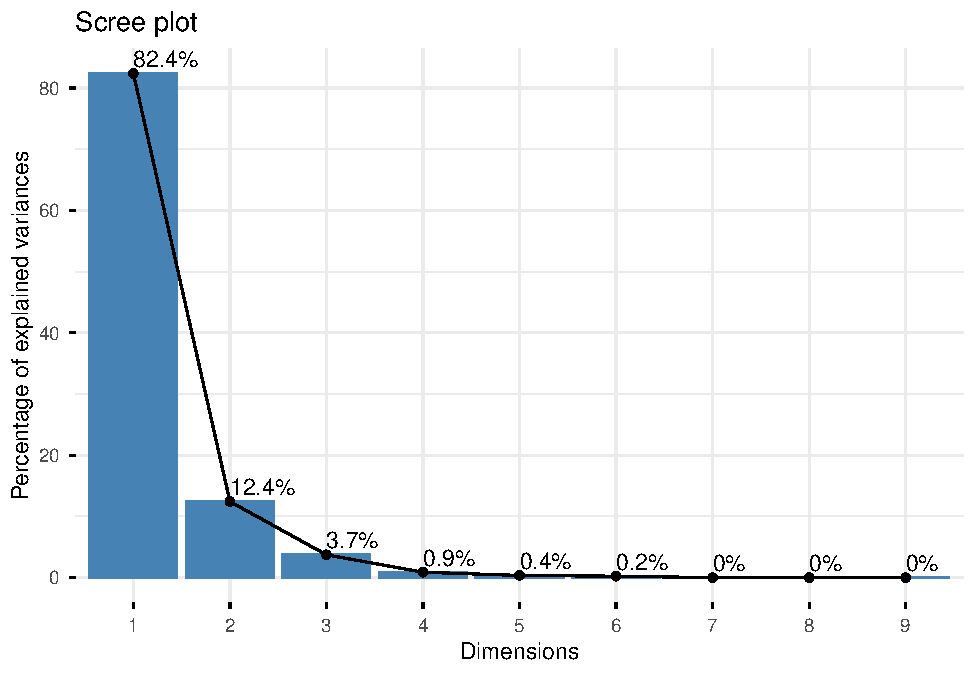
\includegraphics[keepaspectratio]{byHUC12_visual_ChatGPTv2_files/figure-latex/pca-1.pdf}}

\begin{Shaded}
\begin{Highlighting}[]
\FunctionTok{fviz\_pca\_var}\NormalTok{(}
\NormalTok{  pca\_model,}
  \AttributeTok{col.var =} \StringTok{"contrib"}\NormalTok{,}
  \AttributeTok{repel =} \ConstantTok{TRUE}
\NormalTok{)}
\end{Highlighting}
\end{Shaded}

\pandocbounded{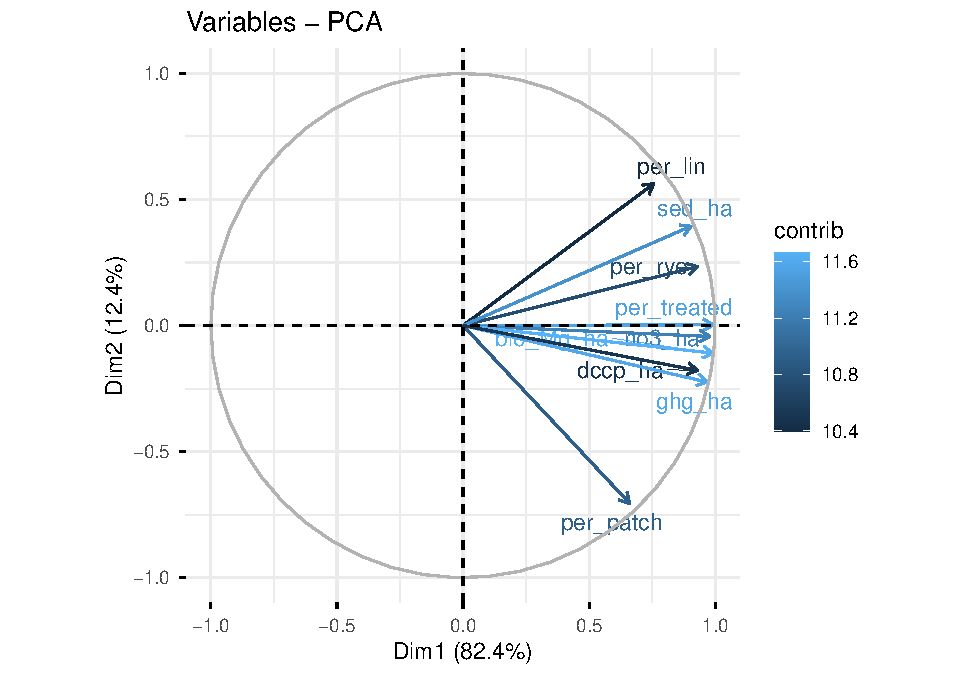
\includegraphics[keepaspectratio]{byHUC12_visual_ChatGPTv2_files/figure-latex/pca-2.pdf}}

\begin{Shaded}
\begin{Highlighting}[]
\CommentTok{\# ============================================================}
\CommentTok{\# NUMBER OF CLUSTERS}
\CommentTok{\# ============================================================}

\CommentTok{\# {-}{-}{-}{-}{-}{-}{-}{-}{-}{-}{-}{-}{-}{-}{-}{-}{-}{-}{-}{-}{-}{-}{-}{-}{-}{-}{-}{-}{-}{-}{-}{-}{-}{-}{-}{-}{-}{-}{-}{-}{-}{-}{-}{-}{-}{-}{-}{-}{-}{-}{-}{-}{-}{-}{-}{-}{-}{-}{-}{-}}
\CommentTok{\# 9. Evaluate candidate numbers of classes}
\CommentTok{\# {-}{-}{-}{-}{-}{-}{-}{-}{-}{-}{-}{-}{-}{-}{-}{-}{-}{-}{-}{-}{-}{-}{-}{-}{-}{-}{-}{-}{-}{-}{-}{-}{-}{-}{-}{-}{-}{-}{-}{-}{-}{-}{-}{-}{-}{-}{-}{-}{-}{-}{-}{-}{-}{-}{-}{-}{-}{-}{-}{-}}
\CommentTok{\#}
\CommentTok{\# We evaluate k = 2 through 6.}
\CommentTok{\#}
\CommentTok{\# WSS is an elbow diagnostic.}
\CommentTok{\# Silhouette width evaluates within/between{-}cluster separation.}
\CommentTok{\#}
\CommentTok{\# Neither metric is used mechanically to select k.}
\CommentTok{\# Cluster size and substantive interpretability are also}
\CommentTok{\# considered.}
\CommentTok{\# {-}{-}{-}{-}{-}{-}{-}{-}{-}{-}{-}{-}{-}{-}{-}{-}{-}{-}{-}{-}{-}{-}{-}{-}{-}{-}{-}{-}{-}{-}{-}{-}{-}{-}{-}{-}{-}{-}{-}{-}{-}{-}{-}{-}{-}{-}{-}{-}{-}{-}{-}{-}{-}{-}{-}{-}{-}{-}{-}{-}}

\FunctionTok{set.seed}\NormalTok{(}\DecValTok{123}\NormalTok{)}

\NormalTok{k\_values }\OtherTok{\textless{}{-}} \DecValTok{2}\SpecialCharTok{:}\DecValTok{6}

\NormalTok{wss\_results }\OtherTok{\textless{}{-}} \FunctionTok{map\_dfr}\NormalTok{(}
\NormalTok{  k\_values,}
  \ControlFlowTok{function}\NormalTok{(k) \{}

\NormalTok{    km }\OtherTok{\textless{}{-}} \FunctionTok{kmeans}\NormalTok{(}
\NormalTok{      cluster\_scaled,}
      \AttributeTok{centers =}\NormalTok{ k,}
      \AttributeTok{nstart =} \DecValTok{100}
\NormalTok{    )}

    \FunctionTok{tibble}\NormalTok{(}
      \AttributeTok{k =}\NormalTok{ k,}
      \AttributeTok{tot\_withinss =}\NormalTok{ km}\SpecialCharTok{$}\NormalTok{tot.withinss}
\NormalTok{    )}
\NormalTok{  \}}
\NormalTok{)}

\FunctionTok{print}\NormalTok{(wss\_results)}
\end{Highlighting}
\end{Shaded}

\begin{verbatim}
## # A tibble: 5 x 2
##       k tot_withinss
##   <int>        <dbl>
## 1     2        173. 
## 2     3        106. 
## 3     4         75.6
## 4     5         57.4
## 5     6         46.6
\end{verbatim}

\begin{Shaded}
\begin{Highlighting}[]
\CommentTok{\# WSS plot}

\FunctionTok{ggplot}\NormalTok{(}
\NormalTok{  wss\_results,}
  \FunctionTok{aes}\NormalTok{(}\AttributeTok{x =}\NormalTok{ k, }\AttributeTok{y =}\NormalTok{ tot\_withinss)}
\NormalTok{) }\SpecialCharTok{+}
  \FunctionTok{geom\_line}\NormalTok{() }\SpecialCharTok{+}
  \FunctionTok{geom\_point}\NormalTok{(}\AttributeTok{size =} \DecValTok{3}\NormalTok{) }\SpecialCharTok{+}
  \FunctionTok{scale\_x\_continuous}\NormalTok{(}\AttributeTok{breaks =}\NormalTok{ k\_values) }\SpecialCharTok{+}
  \FunctionTok{theme\_minimal}\NormalTok{() }\SpecialCharTok{+}
  \FunctionTok{labs}\NormalTok{(}
    \AttributeTok{x =} \StringTok{"Number of planning classes (k)"}\NormalTok{,}
    \AttributeTok{y =} \StringTok{"Total within{-}cluster sum of squares"}
\NormalTok{  )}
\end{Highlighting}
\end{Shaded}

\pandocbounded{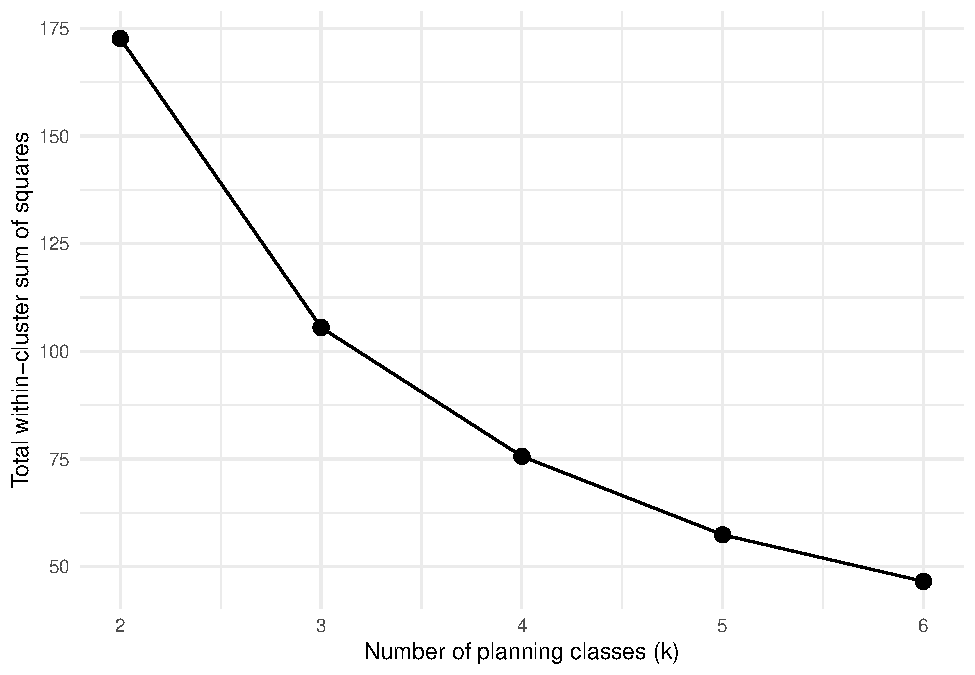
\includegraphics[keepaspectratio]{byHUC12_visual_ChatGPTv2_files/figure-latex/cluster_analysis-1.pdf}}

\begin{Shaded}
\begin{Highlighting}[]
\CommentTok{\# {-}{-}{-}{-}{-}{-}{-}{-}{-}{-}{-}{-}{-}{-}{-}{-}{-}{-}{-}{-}{-}{-}{-}{-}{-}{-}{-}{-}{-}{-}{-}{-}{-}{-}{-}{-}{-}{-}{-}{-}{-}{-}{-}{-}{-}{-}{-}{-}{-}{-}{-}{-}{-}{-}{-}{-}{-}{-}{-}{-}}
\CommentTok{\# 10. Silhouette diagnostics}
\CommentTok{\# {-}{-}{-}{-}{-}{-}{-}{-}{-}{-}{-}{-}{-}{-}{-}{-}{-}{-}{-}{-}{-}{-}{-}{-}{-}{-}{-}{-}{-}{-}{-}{-}{-}{-}{-}{-}{-}{-}{-}{-}{-}{-}{-}{-}{-}{-}{-}{-}{-}{-}{-}{-}{-}{-}{-}{-}{-}{-}{-}{-}}

\NormalTok{distance\_matrix }\OtherTok{\textless{}{-}} \FunctionTok{dist}\NormalTok{(cluster\_scaled)}

\NormalTok{silhouette\_results }\OtherTok{\textless{}{-}} \FunctionTok{map\_dfr}\NormalTok{(}
\NormalTok{  k\_values,}
  \ControlFlowTok{function}\NormalTok{(k) \{}

    \FunctionTok{set.seed}\NormalTok{(}\DecValTok{123}\NormalTok{)}

\NormalTok{    km }\OtherTok{\textless{}{-}} \FunctionTok{kmeans}\NormalTok{(}
\NormalTok{      cluster\_scaled,}
      \AttributeTok{centers =}\NormalTok{ k,}
      \AttributeTok{nstart =} \DecValTok{100}
\NormalTok{    )}

\NormalTok{    sil }\OtherTok{\textless{}{-}} \FunctionTok{silhouette}\NormalTok{(}
\NormalTok{      km}\SpecialCharTok{$}\NormalTok{cluster,}
\NormalTok{      distance\_matrix}
\NormalTok{    )}

    \FunctionTok{tibble}\NormalTok{(}
      \AttributeTok{k =}\NormalTok{ k,}
      \AttributeTok{mean\_silhouette =}
        \FunctionTok{mean}\NormalTok{(sil[, }\StringTok{"sil\_width"}\NormalTok{]),}
      \AttributeTok{median\_silhouette =}
        \FunctionTok{median}\NormalTok{(sil[, }\StringTok{"sil\_width"}\NormalTok{]),}
      \AttributeTok{min\_silhouette =}
        \FunctionTok{min}\NormalTok{(sil[, }\StringTok{"sil\_width"}\NormalTok{]),}
      \AttributeTok{n\_negative =}
        \FunctionTok{sum}\NormalTok{(sil[, }\StringTok{"sil\_width"}\NormalTok{] }\SpecialCharTok{\textless{}} \DecValTok{0}\NormalTok{)}
\NormalTok{    )}
\NormalTok{  \}}
\NormalTok{)}

\FunctionTok{print}\NormalTok{(silhouette\_results)}
\end{Highlighting}
\end{Shaded}

\begin{verbatim}
## # A tibble: 5 x 5
##       k mean_silhouette median_silhouette min_silhouette n_negative
##   <int>           <dbl>             <dbl>          <dbl>      <int>
## 1     2           0.473             0.508         0.134           0
## 2     3           0.433             0.414        -0.0423          1
## 3     4           0.434             0.419        -0.0457          2
## 4     5           0.453             0.456        -0.0981          2
## 5     6           0.396             0.371        -0.0421          3
\end{verbatim}

\begin{Shaded}
\begin{Highlighting}[]
\FunctionTok{write.csv}\NormalTok{(}
\NormalTok{  silhouette\_results,}
  \StringTok{"../data/tidy/silhouette\_diagnostics.csv"}\NormalTok{,}
  \AttributeTok{row.names =} \ConstantTok{FALSE}
\NormalTok{)}


\FunctionTok{ggplot}\NormalTok{(}
\NormalTok{  silhouette\_results,}
  \FunctionTok{aes}\NormalTok{(}\AttributeTok{x =}\NormalTok{ k, }\AttributeTok{y =}\NormalTok{ mean\_silhouette)}
\NormalTok{) }\SpecialCharTok{+}
  \FunctionTok{geom\_line}\NormalTok{() }\SpecialCharTok{+}
  \FunctionTok{geom\_point}\NormalTok{(}\AttributeTok{size =} \DecValTok{3}\NormalTok{) }\SpecialCharTok{+}
  \FunctionTok{scale\_x\_continuous}\NormalTok{(}\AttributeTok{breaks =}\NormalTok{ k\_values) }\SpecialCharTok{+}
  \FunctionTok{theme\_minimal}\NormalTok{() }\SpecialCharTok{+}
  \FunctionTok{labs}\NormalTok{(}
    \AttributeTok{x =} \StringTok{"Number of planning classes (k)"}\NormalTok{,}
    \AttributeTok{y =} \StringTok{"Mean silhouette width"}
\NormalTok{  )}
\end{Highlighting}
\end{Shaded}

\pandocbounded{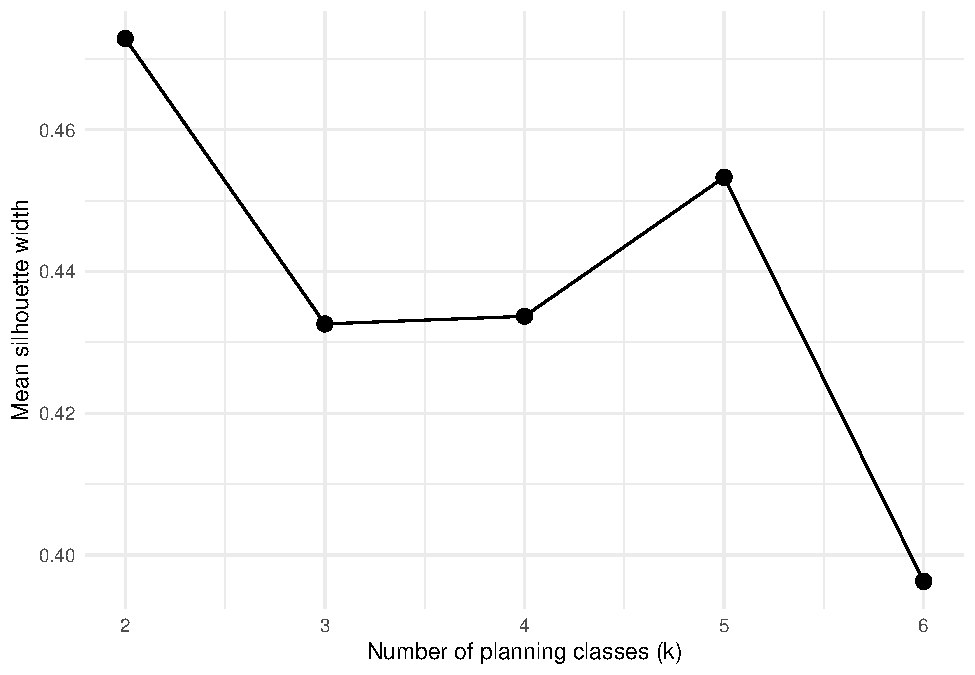
\includegraphics[keepaspectratio]{byHUC12_visual_ChatGPTv2_files/figure-latex/cluster_analysis-2.pdf}}

\begin{Shaded}
\begin{Highlighting}[]
\CommentTok{\# ============================================================}
\CommentTok{\# PRIMARY FIVE{-}CLASS SOLUTION}
\CommentTok{\# ============================================================}

\CommentTok{\# {-}{-}{-}{-}{-}{-}{-}{-}{-}{-}{-}{-}{-}{-}{-}{-}{-}{-}{-}{-}{-}{-}{-}{-}{-}{-}{-}{-}{-}{-}{-}{-}{-}{-}{-}{-}{-}{-}{-}{-}{-}{-}{-}{-}{-}{-}{-}{-}{-}{-}{-}{-}{-}{-}{-}{-}{-}{-}{-}{-}}
\CommentTok{\# 11. Fit primary k{-}means solution}
\CommentTok{\# {-}{-}{-}{-}{-}{-}{-}{-}{-}{-}{-}{-}{-}{-}{-}{-}{-}{-}{-}{-}{-}{-}{-}{-}{-}{-}{-}{-}{-}{-}{-}{-}{-}{-}{-}{-}{-}{-}{-}{-}{-}{-}{-}{-}{-}{-}{-}{-}{-}{-}{-}{-}{-}{-}{-}{-}{-}{-}{-}{-}}
\CommentTok{\#}
\CommentTok{\# Five classes are retained for the primary analysis because}
\CommentTok{\# the five{-}class solution provides an additional meaningful}
\CommentTok{\# distinction in practice configuration while maintaining}
\CommentTok{\# comparable silhouette performance to the four{-}class solution.}
\CommentTok{\#}
\CommentTok{\# IMPORTANT:}
\CommentTok{\# This is a substantive/model{-}selection decision, not a claim}
\CommentTok{\# that five is universally optimal.}
\CommentTok{\# {-}{-}{-}{-}{-}{-}{-}{-}{-}{-}{-}{-}{-}{-}{-}{-}{-}{-}{-}{-}{-}{-}{-}{-}{-}{-}{-}{-}{-}{-}{-}{-}{-}{-}{-}{-}{-}{-}{-}{-}{-}{-}{-}{-}{-}{-}{-}{-}{-}{-}{-}{-}{-}{-}{-}{-}{-}{-}{-}{-}}

\NormalTok{k\_primary }\OtherTok{\textless{}{-}} \DecValTok{5}

\FunctionTok{set.seed}\NormalTok{(}\DecValTok{123}\NormalTok{)}

\NormalTok{km\_model }\OtherTok{\textless{}{-}} \FunctionTok{kmeans}\NormalTok{(}
\NormalTok{  cluster\_scaled,}
  \AttributeTok{centers =}\NormalTok{ k\_primary,}
  \AttributeTok{nstart =} \DecValTok{100}
\NormalTok{)}


\CommentTok{\# {-}{-}{-}{-}{-}{-}{-}{-}{-}{-}{-}{-}{-}{-}{-}{-}{-}{-}{-}{-}{-}{-}{-}{-}{-}{-}{-}{-}{-}{-}{-}{-}{-}{-}{-}{-}{-}{-}{-}{-}{-}{-}{-}{-}{-}{-}{-}{-}{-}{-}{-}{-}{-}{-}{-}{-}{-}{-}{-}{-}}
\CommentTok{\# 12. Add cluster assignment}
\CommentTok{\# {-}{-}{-}{-}{-}{-}{-}{-}{-}{-}{-}{-}{-}{-}{-}{-}{-}{-}{-}{-}{-}{-}{-}{-}{-}{-}{-}{-}{-}{-}{-}{-}{-}{-}{-}{-}{-}{-}{-}{-}{-}{-}{-}{-}{-}{-}{-}{-}{-}{-}{-}{-}{-}{-}{-}{-}{-}{-}{-}{-}}

\NormalTok{huc12\_cluster }\OtherTok{\textless{}{-}}\NormalTok{ huc12\_cluster }\SpecialCharTok{\%\textgreater{}\%}
  \FunctionTok{mutate}\NormalTok{(}
    \AttributeTok{cluster =} \FunctionTok{factor}\NormalTok{(km\_model}\SpecialCharTok{$}\NormalTok{cluster)}
\NormalTok{  )}


\CommentTok{\# {-}{-}{-}{-}{-}{-}{-}{-}{-}{-}{-}{-}{-}{-}{-}{-}{-}{-}{-}{-}{-}{-}{-}{-}{-}{-}{-}{-}{-}{-}{-}{-}{-}{-}{-}{-}{-}{-}{-}{-}{-}{-}{-}{-}{-}{-}{-}{-}{-}{-}{-}{-}{-}{-}{-}{-}{-}{-}{-}{-}}
\CommentTok{\# 13. Cluster sizes}
\CommentTok{\# {-}{-}{-}{-}{-}{-}{-}{-}{-}{-}{-}{-}{-}{-}{-}{-}{-}{-}{-}{-}{-}{-}{-}{-}{-}{-}{-}{-}{-}{-}{-}{-}{-}{-}{-}{-}{-}{-}{-}{-}{-}{-}{-}{-}{-}{-}{-}{-}{-}{-}{-}{-}{-}{-}{-}{-}{-}{-}{-}{-}}

\NormalTok{cluster\_sizes }\OtherTok{\textless{}{-}}\NormalTok{ huc12\_cluster }\SpecialCharTok{\%\textgreater{}\%}
  \FunctionTok{count}\NormalTok{(cluster, }\AttributeTok{name =} \StringTok{"n"}\NormalTok{) }\SpecialCharTok{\%\textgreater{}\%}
  \FunctionTok{mutate}\NormalTok{(}
    \AttributeTok{percent =} \DecValTok{100} \SpecialCharTok{*}\NormalTok{ n }\SpecialCharTok{/} \FunctionTok{sum}\NormalTok{(n)}
\NormalTok{  )}

\FunctionTok{print}\NormalTok{(cluster\_sizes)}
\end{Highlighting}
\end{Shaded}

\begin{verbatim}
## # A tibble: 5 x 3
##   cluster     n percent
##   <fct>   <int>   <dbl>
## 1 1           5    10.6
## 2 2          10    21.3
## 3 3           8    17.0
## 4 4           6    12.8
## 5 5          18    38.3
\end{verbatim}

\begin{Shaded}
\begin{Highlighting}[]
\FunctionTok{write.csv}\NormalTok{(}
\NormalTok{  cluster\_sizes,}
  \StringTok{"../data/tidy/archetype\_cluster\_sizes.csv"}\NormalTok{,}
  \AttributeTok{row.names =} \ConstantTok{FALSE}
\NormalTok{)}


\CommentTok{\# {-}{-}{-}{-}{-}{-}{-}{-}{-}{-}{-}{-}{-}{-}{-}{-}{-}{-}{-}{-}{-}{-}{-}{-}{-}{-}{-}{-}{-}{-}{-}{-}{-}{-}{-}{-}{-}{-}{-}{-}{-}{-}{-}{-}{-}{-}{-}{-}{-}{-}{-}{-}{-}{-}{-}{-}{-}{-}{-}{-}}
\CommentTok{\# 14. Primary clustering diagnostics}
\CommentTok{\# {-}{-}{-}{-}{-}{-}{-}{-}{-}{-}{-}{-}{-}{-}{-}{-}{-}{-}{-}{-}{-}{-}{-}{-}{-}{-}{-}{-}{-}{-}{-}{-}{-}{-}{-}{-}{-}{-}{-}{-}{-}{-}{-}{-}{-}{-}{-}{-}{-}{-}{-}{-}{-}{-}{-}{-}{-}{-}{-}{-}}

\NormalTok{primary\_silhouette }\OtherTok{\textless{}{-}} \FunctionTok{silhouette}\NormalTok{(}
\NormalTok{  km\_model}\SpecialCharTok{$}\NormalTok{cluster,}
\NormalTok{  distance\_matrix}
\NormalTok{)}

\NormalTok{primary\_silhouette\_summary }\OtherTok{\textless{}{-}} \FunctionTok{tibble}\NormalTok{(}
  \AttributeTok{k =}\NormalTok{ k\_primary,}
  \AttributeTok{mean\_silhouette =}
    \FunctionTok{mean}\NormalTok{(primary\_silhouette[, }\StringTok{"sil\_width"}\NormalTok{]),}
  \AttributeTok{median\_silhouette =}
    \FunctionTok{median}\NormalTok{(primary\_silhouette[, }\StringTok{"sil\_width"}\NormalTok{]),}
  \AttributeTok{min\_silhouette =}
    \FunctionTok{min}\NormalTok{(primary\_silhouette[, }\StringTok{"sil\_width"}\NormalTok{]),}
  \AttributeTok{n\_negative =}
    \FunctionTok{sum}\NormalTok{(primary\_silhouette[, }\StringTok{"sil\_width"}\NormalTok{] }\SpecialCharTok{\textless{}} \DecValTok{0}\NormalTok{)}
\NormalTok{)}

\FunctionTok{print}\NormalTok{(primary\_silhouette\_summary)}
\end{Highlighting}
\end{Shaded}

\begin{verbatim}
## # A tibble: 1 x 5
##       k mean_silhouette median_silhouette min_silhouette n_negative
##   <dbl>           <dbl>             <dbl>          <dbl>      <int>
## 1     5           0.453             0.456        -0.0981          2
\end{verbatim}

\begin{Shaded}
\begin{Highlighting}[]
\FunctionTok{write.csv}\NormalTok{(}
\NormalTok{  primary\_silhouette\_summary,}
  \StringTok{"../data/tidy/primary\_silhouette\_summary.csv"}\NormalTok{,}
  \AttributeTok{row.names =} \ConstantTok{FALSE}
\NormalTok{)}


\CommentTok{\# Silhouette plot for the five{-}class solution}

\FunctionTok{fviz\_silhouette}\NormalTok{(}
\NormalTok{  primary\_silhouette}
\NormalTok{)}
\end{Highlighting}
\end{Shaded}

\begin{verbatim}
##   cluster size ave.sil.width
## 1       1    5          0.38
## 2       2   10          0.81
## 3       3    8          0.37
## 4       4    6          0.16
## 5       5   18          0.41
\end{verbatim}

\pandocbounded{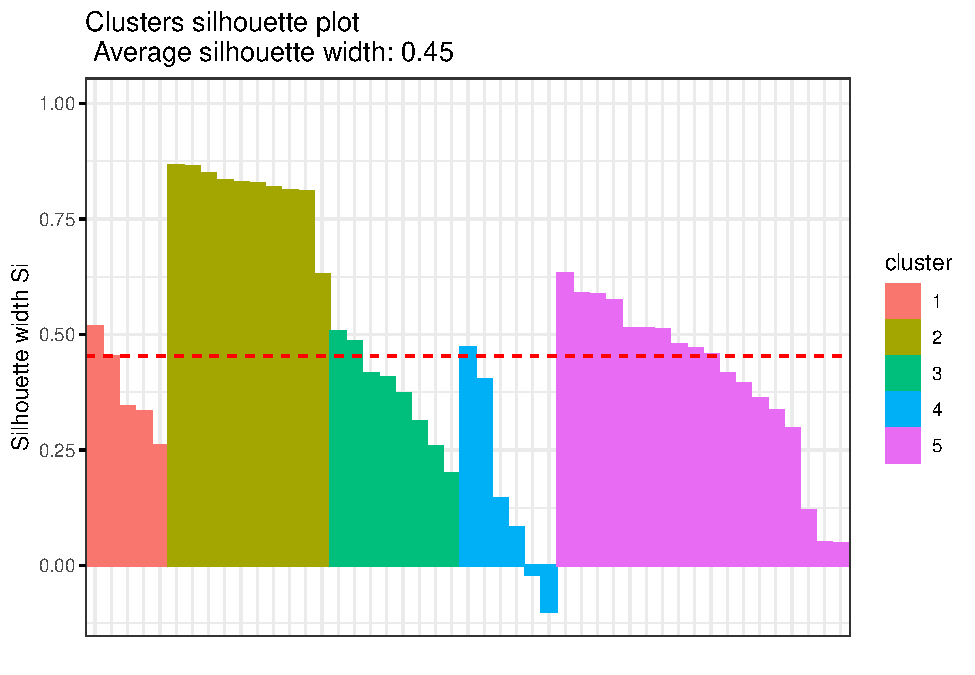
\includegraphics[keepaspectratio]{byHUC12_visual_ChatGPTv2_files/figure-latex/planning_clusters-1.pdf}}

\begin{Shaded}
\begin{Highlighting}[]
\CommentTok{\# ============================================================}
\CommentTok{\# CLUSTER STABILITY SENSITIVITY ANALYSIS}
\CommentTok{\# ============================================================}

\CommentTok{\# {-}{-}{-}{-}{-}{-}{-}{-}{-}{-}{-}{-}{-}{-}{-}{-}{-}{-}{-}{-}{-}{-}{-}{-}{-}{-}{-}{-}{-}{-}{-}{-}{-}{-}{-}{-}{-}{-}{-}{-}{-}{-}{-}{-}{-}{-}{-}{-}{-}{-}{-}{-}{-}{-}{-}{-}{-}{-}{-}{-}}
\CommentTok{\# 15. Repeated k{-}means stability analysis}
\CommentTok{\# {-}{-}{-}{-}{-}{-}{-}{-}{-}{-}{-}{-}{-}{-}{-}{-}{-}{-}{-}{-}{-}{-}{-}{-}{-}{-}{-}{-}{-}{-}{-}{-}{-}{-}{-}{-}{-}{-}{-}{-}{-}{-}{-}{-}{-}{-}{-}{-}{-}{-}{-}{-}{-}{-}{-}{-}{-}{-}{-}{-}}
\CommentTok{\#}
\CommentTok{\# K{-}means solutions can depend on starting values.}
\CommentTok{\#}
\CommentTok{\# We therefore repeat the five{-}class solution using many}
\CommentTok{\# different random seeds and compare the resulting assignments}
\CommentTok{\# to the primary solution using the Adjusted Rand Index (ARI).}
\CommentTok{\#}
\CommentTok{\# ARI:}
\CommentTok{\#   1.0 = identical partition}
\CommentTok{\#   \textasciitilde{}0   = agreement approximately expected by chance}
\CommentTok{\#}
\CommentTok{\# This evaluates stability of the PARTITION, not statistical}
\CommentTok{\# significance of individual variables.}
\CommentTok{\# {-}{-}{-}{-}{-}{-}{-}{-}{-}{-}{-}{-}{-}{-}{-}{-}{-}{-}{-}{-}{-}{-}{-}{-}{-}{-}{-}{-}{-}{-}{-}{-}{-}{-}{-}{-}{-}{-}{-}{-}{-}{-}{-}{-}{-}{-}{-}{-}{-}{-}{-}{-}{-}{-}{-}{-}{-}{-}{-}{-}}

\CommentTok{\# Requires mclust}
\CommentTok{\# install.packages("mclust") if necessary}

\FunctionTok{library}\NormalTok{(mclust)}
\end{Highlighting}
\end{Shaded}

\begin{verbatim}
## Warning: package 'mclust' was built under R version 4.4.3
\end{verbatim}

\begin{verbatim}
## Package 'mclust' version 6.1.2
## Type 'citation("mclust")' for citing this R package in publications.
\end{verbatim}

\begin{verbatim}
## 
## Attaching package: 'mclust'
\end{verbatim}

\begin{verbatim}
## The following object is masked from 'package:dplyr':
## 
##     count
\end{verbatim}

\begin{verbatim}
## The following object is masked from 'package:purrr':
## 
##     map
\end{verbatim}

\begin{Shaded}
\begin{Highlighting}[]
\FunctionTok{set.seed}\NormalTok{(}\DecValTok{123}\NormalTok{)}

\NormalTok{n\_stability\_runs }\OtherTok{\textless{}{-}} \DecValTok{500}

\NormalTok{stability\_results }\OtherTok{\textless{}{-}} \FunctionTok{map\_dfr}\NormalTok{(}
  \FunctionTok{seq\_len}\NormalTok{(n\_stability\_runs),}
  \ControlFlowTok{function}\NormalTok{(i) \{}

\NormalTok{    seed\_i }\OtherTok{\textless{}{-}} \DecValTok{1000} \SpecialCharTok{+}\NormalTok{ i}

    \FunctionTok{set.seed}\NormalTok{(seed\_i)}

\NormalTok{    km\_i }\OtherTok{\textless{}{-}} \FunctionTok{kmeans}\NormalTok{(}
\NormalTok{      cluster\_scaled,}
      \AttributeTok{centers =}\NormalTok{ k\_primary,}
      \AttributeTok{nstart =} \DecValTok{25}
\NormalTok{    )}

\NormalTok{    ari\_i }\OtherTok{\textless{}{-}} \FunctionTok{adjustedRandIndex}\NormalTok{(}
\NormalTok{      km\_model}\SpecialCharTok{$}\NormalTok{cluster,}
\NormalTok{      km\_i}\SpecialCharTok{$}\NormalTok{cluster}
\NormalTok{    )}

    \FunctionTok{tibble}\NormalTok{(}
      \AttributeTok{run =}\NormalTok{ i,}
      \AttributeTok{seed =}\NormalTok{ seed\_i,}
      \AttributeTok{ARI =}\NormalTok{ ari\_i}
\NormalTok{    )}
\NormalTok{  \}}
\NormalTok{)}

\FunctionTok{print}\NormalTok{(}
\NormalTok{  stability\_results }\SpecialCharTok{\%\textgreater{}\%}
    \FunctionTok{summarise}\NormalTok{(}
      \AttributeTok{mean\_ARI =} \FunctionTok{mean}\NormalTok{(ARI),}
      \AttributeTok{median\_ARI =} \FunctionTok{median}\NormalTok{(ARI),}
      \AttributeTok{min\_ARI =} \FunctionTok{min}\NormalTok{(ARI),}
      \AttributeTok{max\_ARI =} \FunctionTok{max}\NormalTok{(ARI),}
      \AttributeTok{sd\_ARI =} \FunctionTok{sd}\NormalTok{(ARI)}
\NormalTok{    )}
\NormalTok{)}
\end{Highlighting}
\end{Shaded}

\begin{verbatim}
## # A tibble: 1 x 5
##   mean_ARI median_ARI min_ARI max_ARI sd_ARI
##      <dbl>      <dbl>   <dbl>   <dbl>  <dbl>
## 1        1          1       1       1      0
\end{verbatim}

\begin{Shaded}
\begin{Highlighting}[]
\FunctionTok{write.csv}\NormalTok{(}
\NormalTok{  stability\_results,}
  \StringTok{"../data/tidy/archetype\_stability\_results.csv"}\NormalTok{,}
  \AttributeTok{row.names =} \ConstantTok{FALSE}
\NormalTok{)}


\CommentTok{\# Stability distribution}

\FunctionTok{ggplot}\NormalTok{(}
\NormalTok{  stability\_results,}
  \FunctionTok{aes}\NormalTok{(}\AttributeTok{x =}\NormalTok{ ARI)}
\NormalTok{) }\SpecialCharTok{+}
  \FunctionTok{geom\_histogram}\NormalTok{(}\AttributeTok{bins =} \DecValTok{30}\NormalTok{) }\SpecialCharTok{+}
  \FunctionTok{geom\_vline}\NormalTok{(}
    \AttributeTok{xintercept =} \FloatTok{0.8}\NormalTok{,}
    \AttributeTok{linetype =} \StringTok{"dashed"}
\NormalTok{  ) }\SpecialCharTok{+}
  \FunctionTok{theme\_minimal}\NormalTok{() }\SpecialCharTok{+}
  \FunctionTok{labs}\NormalTok{(}
    \AttributeTok{x =} \StringTok{"Adjusted Rand Index relative to primary solution"}\NormalTok{,}
    \AttributeTok{y =} \StringTok{"Number of repeated k{-}means runs"}
\NormalTok{  )}
\end{Highlighting}
\end{Shaded}

\pandocbounded{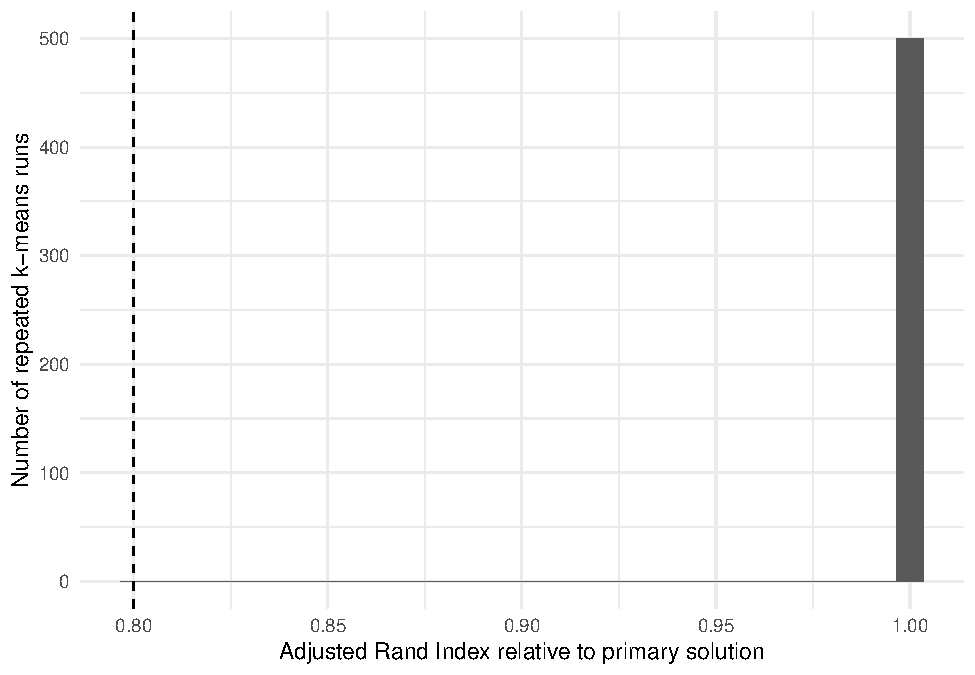
\includegraphics[keepaspectratio]{byHUC12_visual_ChatGPTv2_files/figure-latex/cluster_sens_analysis-1.pdf}}

\begin{Shaded}
\begin{Highlighting}[]
\CommentTok{\# ============================================================}
\CommentTok{\# SENSITIVITY TO NUMBER OF CLASSES}
\CommentTok{\# ============================================================}

\CommentTok{\# {-}{-}{-}{-}{-}{-}{-}{-}{-}{-}{-}{-}{-}{-}{-}{-}{-}{-}{-}{-}{-}{-}{-}{-}{-}{-}{-}{-}{-}{-}{-}{-}{-}{-}{-}{-}{-}{-}{-}{-}{-}{-}{-}{-}{-}{-}{-}{-}{-}{-}{-}{-}{-}{-}{-}{-}{-}{-}{-}{-}}
\CommentTok{\# 16. Compare cluster stability across k}
\CommentTok{\# {-}{-}{-}{-}{-}{-}{-}{-}{-}{-}{-}{-}{-}{-}{-}{-}{-}{-}{-}{-}{-}{-}{-}{-}{-}{-}{-}{-}{-}{-}{-}{-}{-}{-}{-}{-}{-}{-}{-}{-}{-}{-}{-}{-}{-}{-}{-}{-}{-}{-}{-}{-}{-}{-}{-}{-}{-}{-}{-}{-}}
\CommentTok{\#}
\CommentTok{\# This asks whether the selected number of classes is}
\CommentTok{\# particularly unstable relative to nearby alternatives.}
\CommentTok{\# {-}{-}{-}{-}{-}{-}{-}{-}{-}{-}{-}{-}{-}{-}{-}{-}{-}{-}{-}{-}{-}{-}{-}{-}{-}{-}{-}{-}{-}{-}{-}{-}{-}{-}{-}{-}{-}{-}{-}{-}{-}{-}{-}{-}{-}{-}{-}{-}{-}{-}{-}{-}{-}{-}{-}{-}{-}{-}{-}{-}}

\FunctionTok{set.seed}\NormalTok{(}\DecValTok{123}\NormalTok{)}

\NormalTok{k\_stability }\OtherTok{\textless{}{-}} \DecValTok{2}\SpecialCharTok{:}\DecValTok{6}

\NormalTok{k\_stability\_results }\OtherTok{\textless{}{-}} \FunctionTok{map\_dfr}\NormalTok{(}
\NormalTok{  k\_stability,}
  \ControlFlowTok{function}\NormalTok{(k) \{}

    \CommentTok{\# Reference solution}
    \FunctionTok{set.seed}\NormalTok{(}\DecValTok{123}\NormalTok{)}

\NormalTok{    reference }\OtherTok{\textless{}{-}} \FunctionTok{kmeans}\NormalTok{(}
\NormalTok{      cluster\_scaled,}
      \AttributeTok{centers =}\NormalTok{ k,}
      \AttributeTok{nstart =} \DecValTok{100}
\NormalTok{    )}

    \CommentTok{\# Repeated solutions}
\NormalTok{    ari\_values }\OtherTok{\textless{}{-}} \FunctionTok{map\_dbl}\NormalTok{(}
      \DecValTok{1}\SpecialCharTok{:}\DecValTok{100}\NormalTok{,}
      \ControlFlowTok{function}\NormalTok{(i) \{}

        \FunctionTok{set.seed}\NormalTok{(}\DecValTok{5000} \SpecialCharTok{+}\NormalTok{ i)}

\NormalTok{        repeat\_model }\OtherTok{\textless{}{-}} \FunctionTok{kmeans}\NormalTok{(}
\NormalTok{          cluster\_scaled,}
          \AttributeTok{centers =}\NormalTok{ k,}
          \AttributeTok{nstart =} \DecValTok{25}
\NormalTok{        )}

        \FunctionTok{adjustedRandIndex}\NormalTok{(}
\NormalTok{          reference}\SpecialCharTok{$}\NormalTok{cluster,}
\NormalTok{          repeat\_model}\SpecialCharTok{$}\NormalTok{cluster}
\NormalTok{        )}
\NormalTok{      \}}
\NormalTok{    )}

    \FunctionTok{tibble}\NormalTok{(}
      \AttributeTok{k =}\NormalTok{ k,}
      \AttributeTok{mean\_ARI =} \FunctionTok{mean}\NormalTok{(ari\_values),}
      \AttributeTok{median\_ARI =} \FunctionTok{median}\NormalTok{(ari\_values),}
      \AttributeTok{min\_ARI =} \FunctionTok{min}\NormalTok{(ari\_values),}
      \AttributeTok{max\_ARI =} \FunctionTok{max}\NormalTok{(ari\_values),}
      \AttributeTok{sd\_ARI =} \FunctionTok{sd}\NormalTok{(ari\_values)}
\NormalTok{    )}
\NormalTok{  \}}
\NormalTok{)}

\FunctionTok{print}\NormalTok{(k\_stability\_results)}
\end{Highlighting}
\end{Shaded}

\begin{verbatim}
## # A tibble: 5 x 6
##       k mean_ARI median_ARI min_ARI max_ARI sd_ARI
##   <int>    <dbl>      <dbl>   <dbl>   <dbl>  <dbl>
## 1     2    1              1   1           1 0     
## 2     3    1              1   1           1 0     
## 3     4    1              1   1           1 0     
## 4     5    0.999          1   0.868       1 0.0132
## 5     6    1              1   1           1 0
\end{verbatim}

\begin{Shaded}
\begin{Highlighting}[]
\FunctionTok{write.csv}\NormalTok{(}
\NormalTok{  k\_stability\_results,}
  \StringTok{"../data/tidy/k\_stability\_results.csv"}\NormalTok{,}
  \AttributeTok{row.names =} \ConstantTok{FALSE}
\NormalTok{)}


\CommentTok{\# ============================================================}
\CommentTok{\# VARIABLE{-}SET SENSITIVITY ANALYSIS}
\CommentTok{\# ============================================================}

\CommentTok{\# {-}{-}{-}{-}{-}{-}{-}{-}{-}{-}{-}{-}{-}{-}{-}{-}{-}{-}{-}{-}{-}{-}{-}{-}{-}{-}{-}{-}{-}{-}{-}{-}{-}{-}{-}{-}{-}{-}{-}{-}{-}{-}{-}{-}{-}{-}{-}{-}{-}{-}{-}{-}{-}{-}{-}{-}{-}{-}{-}{-}}
\CommentTok{\# 17. Define alternative classification variable sets}
\CommentTok{\# {-}{-}{-}{-}{-}{-}{-}{-}{-}{-}{-}{-}{-}{-}{-}{-}{-}{-}{-}{-}{-}{-}{-}{-}{-}{-}{-}{-}{-}{-}{-}{-}{-}{-}{-}{-}{-}{-}{-}{-}{-}{-}{-}{-}{-}{-}{-}{-}{-}{-}{-}{-}{-}{-}{-}{-}{-}{-}{-}{-}}
\CommentTok{\#}
\CommentTok{\# The primary model contains strongly correlated variables.}
\CommentTok{\# This is not necessarily inappropriate because the variables}
\CommentTok{\# represent different planning dimensions, but it is important}
\CommentTok{\# to determine whether the five{-}class solution depends heavily}
\CommentTok{\# on particular variables.}
\CommentTok{\#}
\CommentTok{\# Sensitivity sets:}
\CommentTok{\#}
\CommentTok{\# A = Primary model}
\CommentTok{\#}
\CommentTok{\# B = Remove landscape transformation extent}
\CommentTok{\#     (per\_treated)}
\CommentTok{\#}
\CommentTok{\# C = Remove highly correlated transformation/biomass variables}
\CommentTok{\#     (per\_treated + bio\_Mg\_ha)}
\CommentTok{\#}
\CommentTok{\# D = Remove direct cost}
\CommentTok{\#}
\CommentTok{\# E = Practice/outcome configuration without direct cost and}
\CommentTok{\#     biomass}
\CommentTok{\#}
\CommentTok{\# These are sensitivity analyses, not alternative "correct"}
\CommentTok{\# models.}
\CommentTok{\# {-}{-}{-}{-}{-}{-}{-}{-}{-}{-}{-}{-}{-}{-}{-}{-}{-}{-}{-}{-}{-}{-}{-}{-}{-}{-}{-}{-}{-}{-}{-}{-}{-}{-}{-}{-}{-}{-}{-}{-}{-}{-}{-}{-}{-}{-}{-}{-}{-}{-}{-}{-}{-}{-}{-}{-}{-}{-}{-}{-}}

\NormalTok{variable\_sets }\OtherTok{\textless{}{-}} \FunctionTok{list}\NormalTok{(}

  \AttributeTok{Primary =} \FunctionTok{c}\NormalTok{(}
    \StringTok{"per\_treated"}\NormalTok{,}
    \StringTok{"per\_patch"}\NormalTok{,}
    \StringTok{"per\_lin"}\NormalTok{,}
    \StringTok{"per\_rye"}\NormalTok{,}
    \StringTok{"no3\_ha"}\NormalTok{,}
    \StringTok{"sed\_ha"}\NormalTok{,}
    \StringTok{"ghg\_ha"}\NormalTok{,}
    \StringTok{"bio\_Mg\_ha"}\NormalTok{,}
    \StringTok{"dccp\_ha"}
\NormalTok{  ),}

  \AttributeTok{No\_Treatment\_Extent =} \FunctionTok{c}\NormalTok{(}
    \StringTok{"per\_patch"}\NormalTok{,}
    \StringTok{"per\_lin"}\NormalTok{,}
    \StringTok{"per\_rye"}\NormalTok{,}
    \StringTok{"no3\_ha"}\NormalTok{,}
    \StringTok{"sed\_ha"}\NormalTok{,}
    \StringTok{"ghg\_ha"}\NormalTok{,}
    \StringTok{"bio\_Mg\_ha"}\NormalTok{,}
    \StringTok{"dccp\_ha"}
\NormalTok{  ),}

  \AttributeTok{No\_Treatment\_Extent\_or\_Biomass =} \FunctionTok{c}\NormalTok{(}
    \StringTok{"per\_patch"}\NormalTok{,}
    \StringTok{"per\_lin"}\NormalTok{,}
    \StringTok{"per\_rye"}\NormalTok{,}
    \StringTok{"no3\_ha"}\NormalTok{,}
    \StringTok{"sed\_ha"}\NormalTok{,}
    \StringTok{"ghg\_ha"}\NormalTok{,}
    \StringTok{"dccp\_ha"}
\NormalTok{  ),}

  \AttributeTok{No\_Direct\_Cost =} \FunctionTok{c}\NormalTok{(}
    \StringTok{"per\_treated"}\NormalTok{,}
    \StringTok{"per\_patch"}\NormalTok{,}
    \StringTok{"per\_lin"}\NormalTok{,}
    \StringTok{"per\_rye"}\NormalTok{,}
    \StringTok{"no3\_ha"}\NormalTok{,}
    \StringTok{"sed\_ha"}\NormalTok{,}
    \StringTok{"ghg\_ha"}\NormalTok{,}
    \StringTok{"bio\_Mg\_ha"}
\NormalTok{  ),}

  \AttributeTok{Configuration\_and\_Outcome =} \FunctionTok{c}\NormalTok{(}
    \StringTok{"per\_patch"}\NormalTok{,}
    \StringTok{"per\_lin"}\NormalTok{,}
    \StringTok{"per\_rye"}\NormalTok{,}
    \StringTok{"no3\_ha"}\NormalTok{,}
    \StringTok{"sed\_ha"}\NormalTok{,}
    \StringTok{"ghg\_ha"}
\NormalTok{  )}
\NormalTok{)}


\CommentTok{\# {-}{-}{-}{-}{-}{-}{-}{-}{-}{-}{-}{-}{-}{-}{-}{-}{-}{-}{-}{-}{-}{-}{-}{-}{-}{-}{-}{-}{-}{-}{-}{-}{-}{-}{-}{-}{-}{-}{-}{-}{-}{-}{-}{-}{-}{-}{-}{-}{-}{-}{-}{-}{-}{-}{-}{-}{-}{-}{-}{-}}
\CommentTok{\# 18. Run sensitivity models}
\CommentTok{\# {-}{-}{-}{-}{-}{-}{-}{-}{-}{-}{-}{-}{-}{-}{-}{-}{-}{-}{-}{-}{-}{-}{-}{-}{-}{-}{-}{-}{-}{-}{-}{-}{-}{-}{-}{-}{-}{-}{-}{-}{-}{-}{-}{-}{-}{-}{-}{-}{-}{-}{-}{-}{-}{-}{-}{-}{-}{-}{-}{-}}

\NormalTok{sensitivity\_models }\OtherTok{\textless{}{-}} \FunctionTok{list}\NormalTok{()}

\NormalTok{sensitivity\_summary }\OtherTok{\textless{}{-}} \FunctionTok{map\_dfr}\NormalTok{(}
  \FunctionTok{names}\NormalTok{(variable\_sets),}
  \ControlFlowTok{function}\NormalTok{(model\_name) \{}

\NormalTok{    vars }\OtherTok{\textless{}{-}}\NormalTok{ variable\_sets[[model\_name]]}

\NormalTok{    dat }\OtherTok{\textless{}{-}}\NormalTok{ huc12\_planning }\SpecialCharTok{\%\textgreater{}\%}
      \FunctionTok{select}\NormalTok{(}\FunctionTok{all\_of}\NormalTok{(vars)) }\SpecialCharTok{\%\textgreater{}\%}
      \FunctionTok{filter}\NormalTok{(}\FunctionTok{complete.cases}\NormalTok{(.))}

\NormalTok{    scaled\_dat }\OtherTok{\textless{}{-}} \FunctionTok{scale}\NormalTok{(dat)}

    \FunctionTok{set.seed}\NormalTok{(}\DecValTok{123}\NormalTok{)}

\NormalTok{    km }\OtherTok{\textless{}{-}} \FunctionTok{kmeans}\NormalTok{(}
\NormalTok{      scaled\_dat,}
      \AttributeTok{centers =}\NormalTok{ k\_primary,}
      \AttributeTok{nstart =} \DecValTok{100}
\NormalTok{    )}

\NormalTok{    sil }\OtherTok{\textless{}{-}} \FunctionTok{silhouette}\NormalTok{(}
\NormalTok{      km}\SpecialCharTok{$}\NormalTok{cluster,}
      \FunctionTok{dist}\NormalTok{(scaled\_dat)}
\NormalTok{    )}

    \CommentTok{\# Store model for later comparison}
\NormalTok{    sensitivity\_models[[model\_name]] }\OtherTok{\textless{}\textless{}{-}} \FunctionTok{list}\NormalTok{(}
      \AttributeTok{variables =}\NormalTok{ vars,}
      \AttributeTok{data =}\NormalTok{ dat,}
      \AttributeTok{scaled =}\NormalTok{ scaled\_dat,}
      \AttributeTok{model =}\NormalTok{ km}
\NormalTok{    )}

    \FunctionTok{tibble}\NormalTok{(}
      \AttributeTok{variable\_set =}\NormalTok{ model\_name,}
      \AttributeTok{n\_variables =} \FunctionTok{length}\NormalTok{(vars),}
      \AttributeTok{n\_HUC12 =} \FunctionTok{nrow}\NormalTok{(dat),}
      \AttributeTok{mean\_silhouette =}
        \FunctionTok{mean}\NormalTok{(sil[, }\StringTok{"sil\_width"}\NormalTok{]),}
      \AttributeTok{median\_silhouette =}
        \FunctionTok{median}\NormalTok{(sil[, }\StringTok{"sil\_width"}\NormalTok{]),}
      \AttributeTok{min\_silhouette =}
        \FunctionTok{min}\NormalTok{(sil[, }\StringTok{"sil\_width"}\NormalTok{]),}
      \AttributeTok{n\_negative =}
        \FunctionTok{sum}\NormalTok{(sil[, }\StringTok{"sil\_width"}\NormalTok{] }\SpecialCharTok{\textless{}} \DecValTok{0}\NormalTok{)}
\NormalTok{    )}
\NormalTok{  \}}
\NormalTok{)}

\FunctionTok{print}\NormalTok{(sensitivity\_summary)}
\end{Highlighting}
\end{Shaded}

\begin{verbatim}
## # A tibble: 5 x 7
##   variable_set                   n_variables n_HUC12 mean_silhouette median_silhouette min_silhouette n_negative
##   <chr>                                <int>   <int>           <dbl>             <dbl>          <dbl>      <int>
## 1 Primary                                  9      47           0.453             0.456        -0.0981          2
## 2 No_Treatment_Extent                      8      47           0.457             0.434         0.0341          0
## 3 No_Treatment_Extent_or_Biomass           7      47           0.452             0.442         0.0277          0
## 4 No_Direct_Cost                           8      47           0.465             0.466        -0.0822          1
## 5 Configuration_and_Outcome                6      47           0.454             0.477         0.0625          0
\end{verbatim}

\begin{Shaded}
\begin{Highlighting}[]
\FunctionTok{write.csv}\NormalTok{(}
\NormalTok{  sensitivity\_summary,}
  \StringTok{"../data/tidy/archetype\_variable\_sensitivity.csv"}\NormalTok{,}
  \AttributeTok{row.names =} \ConstantTok{FALSE}
\NormalTok{)}
\end{Highlighting}
\end{Shaded}

\begin{Shaded}
\begin{Highlighting}[]
\CommentTok{\# ============================================================}
\CommentTok{\# 19. Compare alternative variable sets with PRIMARY solution}
\CommentTok{\# ============================================================}

\NormalTok{variable\_set\_ARI }\OtherTok{\textless{}{-}} \FunctionTok{map\_dfr}\NormalTok{(}
  \FunctionTok{names}\NormalTok{(sensitivity\_models),}
  \ControlFlowTok{function}\NormalTok{(model\_name) \{}

\NormalTok{    vars }\OtherTok{\textless{}{-}}\NormalTok{ sensitivity\_models[[model\_name]]}\SpecialCharTok{$}\NormalTok{variables}

    \CommentTok{\# HUC12s with complete data for this variable set}
\NormalTok{    sensitivity\_data }\OtherTok{\textless{}{-}}\NormalTok{ huc12\_planning }\SpecialCharTok{\%\textgreater{}\%}
      \FunctionTok{select}\NormalTok{(HUC12, }\FunctionTok{all\_of}\NormalTok{(vars)) }\SpecialCharTok{\%\textgreater{}\%}
      \FunctionTok{filter}\NormalTok{(}\FunctionTok{complete.cases}\NormalTok{(.)) }\SpecialCharTok{\%\textgreater{}\%}
      \FunctionTok{arrange}\NormalTok{(HUC12)}

    \CommentTok{\# Primary classifications for exactly the same HUC12s}
\NormalTok{    primary\_data }\OtherTok{\textless{}{-}}\NormalTok{ huc12\_cluster }\SpecialCharTok{\%\textgreater{}\%}
      \FunctionTok{select}\NormalTok{(HUC12, }\AttributeTok{primary\_cluster =}\NormalTok{ cluster) }\SpecialCharTok{\%\textgreater{}\%}
      \FunctionTok{filter}\NormalTok{(HUC12 }\SpecialCharTok{\%in\%}\NormalTok{ sensitivity\_data}\SpecialCharTok{$}\NormalTok{HUC12) }\SpecialCharTok{\%\textgreater{}\%}
      \FunctionTok{arrange}\NormalTok{(HUC12)}

    \CommentTok{\# Refit sensitivity model using exactly these HUC12s}
\NormalTok{    x }\OtherTok{\textless{}{-}}\NormalTok{ sensitivity\_data }\SpecialCharTok{\%\textgreater{}\%}
      \FunctionTok{select}\NormalTok{(}\FunctionTok{all\_of}\NormalTok{(vars))}

\NormalTok{    x\_scaled }\OtherTok{\textless{}{-}} \FunctionTok{scale}\NormalTok{(x)}

    \FunctionTok{set.seed}\NormalTok{(}\DecValTok{123}\NormalTok{)}

\NormalTok{    km\_sens }\OtherTok{\textless{}{-}} \FunctionTok{kmeans}\NormalTok{(}
\NormalTok{      x\_scaled,}
      \AttributeTok{centers =}\NormalTok{ k\_primary,}
      \AttributeTok{nstart =} \DecValTok{100}
\NormalTok{    )}

    \FunctionTok{tibble}\NormalTok{(}
      \AttributeTok{variable\_set =}\NormalTok{ model\_name,}
      \AttributeTok{n\_HUC12\_compared =} \FunctionTok{nrow}\NormalTok{(sensitivity\_data),}
      \AttributeTok{ARI\_vs\_primary =}
        \FunctionTok{adjustedRandIndex}\NormalTok{(}
\NormalTok{          primary\_data}\SpecialCharTok{$}\NormalTok{primary\_cluster,}
\NormalTok{          km\_sens}\SpecialCharTok{$}\NormalTok{cluster}
\NormalTok{        )}
\NormalTok{    )}
\NormalTok{  \}}
\NormalTok{)}

\FunctionTok{print}\NormalTok{(variable\_set\_ARI)}
\end{Highlighting}
\end{Shaded}

\begin{verbatim}
## # A tibble: 5 x 3
##   variable_set                   n_HUC12_compared ARI_vs_primary
##   <chr>                                     <int>          <dbl>
## 1 Primary                                      47          1    
## 2 No_Treatment_Extent                          47          0.868
## 3 No_Treatment_Extent_or_Biomass               47          0.868
## 4 No_Direct_Cost                               47          0.868
## 5 Configuration_and_Outcome                    47          0.799
\end{verbatim}

\begin{Shaded}
\begin{Highlighting}[]
\FunctionTok{write.csv}\NormalTok{(}
\NormalTok{  variable\_set\_ARI,}
  \StringTok{"../data/tidy/archetype\_variable\_set\_ARI.csv"}\NormalTok{,}
  \AttributeTok{row.names =} \ConstantTok{FALSE}
\NormalTok{)}
\end{Highlighting}
\end{Shaded}

\begin{Shaded}
\begin{Highlighting}[]
\CommentTok{\# ============================================================}
\CommentTok{\# PCA{-}SCORE SENSITIVITY ANALYSIS}
\CommentTok{\# ============================================================}

\CommentTok{\# {-}{-}{-}{-}{-}{-}{-}{-}{-}{-}{-}{-}{-}{-}{-}{-}{-}{-}{-}{-}{-}{-}{-}{-}{-}{-}{-}{-}{-}{-}{-}{-}{-}{-}{-}{-}{-}{-}{-}{-}{-}{-}{-}{-}{-}{-}{-}{-}{-}{-}{-}{-}{-}{-}{-}{-}{-}{-}{-}{-}}
\CommentTok{\# 20. Cluster on PCA scores as a sensitivity analysis}
\CommentTok{\# {-}{-}{-}{-}{-}{-}{-}{-}{-}{-}{-}{-}{-}{-}{-}{-}{-}{-}{-}{-}{-}{-}{-}{-}{-}{-}{-}{-}{-}{-}{-}{-}{-}{-}{-}{-}{-}{-}{-}{-}{-}{-}{-}{-}{-}{-}{-}{-}{-}{-}{-}{-}{-}{-}{-}{-}{-}{-}{-}{-}}
\CommentTok{\#}
\CommentTok{\# This directly addresses an important methodological question:}
\CommentTok{\#}
\CommentTok{\# Does the classification change substantially if highly}
\CommentTok{\# correlated original variables are first reduced to a smaller}
\CommentTok{\# number of principal components?}
\CommentTok{\#}
\CommentTok{\# The PRIMARY classification remains based on the standardized}
\CommentTok{\# original variables.}
\CommentTok{\# {-}{-}{-}{-}{-}{-}{-}{-}{-}{-}{-}{-}{-}{-}{-}{-}{-}{-}{-}{-}{-}{-}{-}{-}{-}{-}{-}{-}{-}{-}{-}{-}{-}{-}{-}{-}{-}{-}{-}{-}{-}{-}{-}{-}{-}{-}{-}{-}{-}{-}{-}{-}{-}{-}{-}{-}{-}{-}{-}{-}}

\CommentTok{\# Determine number of PCs explaining at least 90\% of variance}

\NormalTok{n\_pc\_90 }\OtherTok{\textless{}{-}} \FunctionTok{which}\NormalTok{(}
\NormalTok{  pca\_variance}\SpecialCharTok{$}\NormalTok{cumulative\_percent }\SpecialCharTok{\textgreater{}=} \DecValTok{90}
\NormalTok{)[}\DecValTok{1}\NormalTok{]}

\FunctionTok{cat}\NormalTok{(}
  \StringTok{"}\SpecialCharTok{\textbackslash{}n}\StringTok{Number of PCs explaining \textgreater{}=90\% of variance:"}\NormalTok{,}
\NormalTok{  n\_pc\_90,}
  \StringTok{"}\SpecialCharTok{\textbackslash{}n}\StringTok{"}
\NormalTok{)}
\end{Highlighting}
\end{Shaded}

\begin{verbatim}
## 
## Number of PCs explaining >=90% of variance: 2
\end{verbatim}

\begin{Shaded}
\begin{Highlighting}[]
\NormalTok{pca\_scores\_90 }\OtherTok{\textless{}{-}}\NormalTok{ pca\_model}\SpecialCharTok{$}\NormalTok{x[, }\FunctionTok{seq\_len}\NormalTok{(n\_pc\_90), drop }\OtherTok{=} \ConstantTok{FALSE}\NormalTok{]}

\FunctionTok{set.seed}\NormalTok{(}\DecValTok{123}\NormalTok{)}

\NormalTok{km\_pca }\OtherTok{\textless{}{-}} \FunctionTok{kmeans}\NormalTok{(}
\NormalTok{  pca\_scores\_90,}
  \AttributeTok{centers =}\NormalTok{ k\_primary,}
  \AttributeTok{nstart =} \DecValTok{100}
\NormalTok{)}

\NormalTok{pca\_silhouette }\OtherTok{\textless{}{-}} \FunctionTok{silhouette}\NormalTok{(}
\NormalTok{  km\_pca}\SpecialCharTok{$}\NormalTok{cluster,}
  \FunctionTok{dist}\NormalTok{(pca\_scores\_90)}
\NormalTok{)}

\NormalTok{pca\_sensitivity\_summary }\OtherTok{\textless{}{-}} \FunctionTok{tibble}\NormalTok{(}
  \AttributeTok{model =} \FunctionTok{paste0}\NormalTok{(}
    \StringTok{"PCA scores ("}\NormalTok{,}
\NormalTok{    n\_pc\_90,}
    \StringTok{" PCs)"}
\NormalTok{  ),}
  \AttributeTok{n\_PC =}\NormalTok{ n\_pc\_90,}
  \AttributeTok{variance\_explained =}
\NormalTok{    pca\_variance}\SpecialCharTok{$}\NormalTok{cumulative\_percent[n\_pc\_90],}
  \AttributeTok{mean\_silhouette =}
    \FunctionTok{mean}\NormalTok{(pca\_silhouette[, }\StringTok{"sil\_width"}\NormalTok{]),}
  \AttributeTok{median\_silhouette =}
    \FunctionTok{median}\NormalTok{(pca\_silhouette[, }\StringTok{"sil\_width"}\NormalTok{]),}
  \AttributeTok{min\_silhouette =}
    \FunctionTok{min}\NormalTok{(pca\_silhouette[, }\StringTok{"sil\_width"}\NormalTok{])}
\NormalTok{)}

\FunctionTok{print}\NormalTok{(pca\_sensitivity\_summary)}
\end{Highlighting}
\end{Shaded}

\begin{verbatim}
## # A tibble: 1 x 6
##   model               n_PC variance_explained mean_silhouette median_silhouette min_silhouette
##   <chr>              <int>              <dbl>           <dbl>             <dbl>          <dbl>
## 1 PCA scores (2 PCs)     2               94.8           0.503             0.507         0.0444
\end{verbatim}

\begin{Shaded}
\begin{Highlighting}[]
\CommentTok{\# Compare PCA solution with primary solution}

\NormalTok{pca\_primary\_ARI }\OtherTok{\textless{}{-}} \FunctionTok{adjustedRandIndex}\NormalTok{(}
\NormalTok{  km\_model}\SpecialCharTok{$}\NormalTok{cluster,}
\NormalTok{  km\_pca}\SpecialCharTok{$}\NormalTok{cluster}
\NormalTok{)}

\FunctionTok{cat}\NormalTok{(}
  \StringTok{"}\SpecialCharTok{\textbackslash{}n}\StringTok{Adjusted Rand Index: primary vs PCA{-}score solution ="}\NormalTok{,}
  \FunctionTok{round}\NormalTok{(pca\_primary\_ARI, }\DecValTok{3}\NormalTok{),}
  \StringTok{"}\SpecialCharTok{\textbackslash{}n}\StringTok{"}
\NormalTok{)}
\end{Highlighting}
\end{Shaded}

\begin{verbatim}
## 
## Adjusted Rand Index: primary vs PCA-score solution = 0.824
\end{verbatim}

\begin{Shaded}
\begin{Highlighting}[]
\FunctionTok{write.csv}\NormalTok{(}
\NormalTok{  pca\_sensitivity\_summary,}
  \StringTok{"../data/tidy/pca\_cluster\_sensitivity.csv"}\NormalTok{,}
  \AttributeTok{row.names =} \ConstantTok{FALSE}
\NormalTok{)}
\end{Highlighting}
\end{Shaded}

\begin{Shaded}
\begin{Highlighting}[]
\CommentTok{\# ============================================================}
\CommentTok{\# 21. Overall sensitivity summary}
\CommentTok{\# ============================================================}

\NormalTok{overall\_sensitivity }\OtherTok{\textless{}{-}} \FunctionTok{bind\_rows}\NormalTok{(}

\NormalTok{  sensitivity\_summary }\SpecialCharTok{\%\textgreater{}\%}
    \FunctionTok{mutate}\NormalTok{(}
      \AttributeTok{analysis\_type =} \StringTok{"Variable set"}
\NormalTok{    ) }\SpecialCharTok{\%\textgreater{}\%}
    \FunctionTok{select}\NormalTok{(}
\NormalTok{      analysis\_type,}
      \AttributeTok{model =}\NormalTok{ variable\_set,}
\NormalTok{      n\_variables,}
\NormalTok{      n\_HUC12,}
\NormalTok{      mean\_silhouette,}
\NormalTok{      median\_silhouette,}
\NormalTok{      min\_silhouette,}
\NormalTok{      n\_negative}
\NormalTok{    ),}

\NormalTok{  pca\_sensitivity\_summary }\SpecialCharTok{\%\textgreater{}\%}
    \FunctionTok{mutate}\NormalTok{(}
      \AttributeTok{analysis\_type =} \StringTok{"PCA score sensitivity"}\NormalTok{,}
      \AttributeTok{n\_variables =}\NormalTok{ n\_PC,}
      \AttributeTok{n\_HUC12 =} \FunctionTok{nrow}\NormalTok{(pca\_scores\_90),}
      \AttributeTok{n\_negative =}
        \FunctionTok{sum}\NormalTok{(pca\_silhouette[, }\StringTok{"sil\_width"}\NormalTok{] }\SpecialCharTok{\textless{}} \DecValTok{0}\NormalTok{)}
\NormalTok{    ) }\SpecialCharTok{\%\textgreater{}\%}
    \FunctionTok{select}\NormalTok{(}
\NormalTok{      analysis\_type,}
\NormalTok{      model,}
\NormalTok{      n\_variables,}
\NormalTok{      n\_HUC12,}
\NormalTok{      mean\_silhouette,}
\NormalTok{      median\_silhouette,}
\NormalTok{      min\_silhouette,}
\NormalTok{      n\_negative}
\NormalTok{    )}
\NormalTok{)}

\FunctionTok{print}\NormalTok{(overall\_sensitivity)}
\end{Highlighting}
\end{Shaded}

\begin{verbatim}
## # A tibble: 6 x 8
##   analysis_type         model                          n_variables n_HUC12 mean_silhouette median_silhouette min_silhouette n_negative
##   <chr>                 <chr>                                <int>   <int>           <dbl>             <dbl>          <dbl>      <int>
## 1 Variable set          Primary                                  9      47           0.453             0.456        -0.0981          2
## 2 Variable set          No_Treatment_Extent                      8      47           0.457             0.434         0.0341          0
## 3 Variable set          No_Treatment_Extent_or_Biomass           7      47           0.452             0.442         0.0277          0
## 4 Variable set          No_Direct_Cost                           8      47           0.465             0.466        -0.0822          1
## 5 Variable set          Configuration_and_Outcome                6      47           0.454             0.477         0.0625          0
## 6 PCA score sensitivity PCA scores (2 PCs)                       2      47           0.503             0.507         0.0444          0
\end{verbatim}

\begin{Shaded}
\begin{Highlighting}[]
\FunctionTok{write.csv}\NormalTok{(}
\NormalTok{  overall\_sensitivity,}
  \StringTok{"../data/tidy/archetype\_overall\_sensitivity.csv"}\NormalTok{,}
  \AttributeTok{row.names =} \ConstantTok{FALSE}
\NormalTok{)}


\CommentTok{\# ============================================================}
\CommentTok{\# 22. Visualize primary planning classes}
\CommentTok{\# ============================================================}

\NormalTok{huc12\_planning }\OtherTok{\textless{}{-}}\NormalTok{ huc12\_cluster }\SpecialCharTok{\%\textgreater{}\%}
  \FunctionTok{mutate}\NormalTok{(}
    \AttributeTok{Planning\_Class =}
      \FunctionTok{paste0}\NormalTok{(}\StringTok{"Planning class "}\NormalTok{, cluster)}
\NormalTok{  )}


\CommentTok{\# {-}{-}{-}{-}{-}{-}{-}{-}{-}{-}{-}{-}{-}{-}{-}{-}{-}{-}{-}{-}{-}{-}{-}{-}{-}{-}{-}{-}{-}{-}{-}{-}{-}{-}{-}{-}{-}{-}{-}{-}{-}{-}{-}{-}{-}{-}{-}{-}{-}{-}{-}{-}{-}{-}{-}{-}{-}{-}{-}{-}}
\CommentTok{\# Join classifications back to complete HUC12 dataset}
\CommentTok{\# {-}{-}{-}{-}{-}{-}{-}{-}{-}{-}{-}{-}{-}{-}{-}{-}{-}{-}{-}{-}{-}{-}{-}{-}{-}{-}{-}{-}{-}{-}{-}{-}{-}{-}{-}{-}{-}{-}{-}{-}{-}{-}{-}{-}{-}{-}{-}{-}{-}{-}{-}{-}{-}{-}{-}{-}{-}{-}{-}{-}}

\NormalTok{huc12\_planning }\OtherTok{\textless{}{-}}\NormalTok{ huc12\_df }\SpecialCharTok{\%\textgreater{}\%}
  \FunctionTok{left\_join}\NormalTok{(}
\NormalTok{    huc12\_planning }\SpecialCharTok{\%\textgreater{}\%}
      \FunctionTok{select}\NormalTok{(}
\NormalTok{        HUC12,}
\NormalTok{        cluster,}
\NormalTok{        Planning\_Class}
\NormalTok{      ),}
    \AttributeTok{by =} \StringTok{"HUC12"}
\NormalTok{  )}


\CommentTok{\# {-}{-}{-}{-}{-}{-}{-}{-}{-}{-}{-}{-}{-}{-}{-}{-}{-}{-}{-}{-}{-}{-}{-}{-}{-}{-}{-}{-}{-}{-}{-}{-}{-}{-}{-}{-}{-}{-}{-}{-}{-}{-}{-}{-}{-}{-}{-}{-}{-}{-}{-}{-}{-}{-}{-}{-}{-}{-}{-}{-}}
\CommentTok{\# Cluster visualization}
\CommentTok{\# {-}{-}{-}{-}{-}{-}{-}{-}{-}{-}{-}{-}{-}{-}{-}{-}{-}{-}{-}{-}{-}{-}{-}{-}{-}{-}{-}{-}{-}{-}{-}{-}{-}{-}{-}{-}{-}{-}{-}{-}{-}{-}{-}{-}{-}{-}{-}{-}{-}{-}{-}{-}{-}{-}{-}{-}{-}{-}{-}{-}}

\FunctionTok{fviz\_cluster}\NormalTok{(}
\NormalTok{  km\_model,}
  \AttributeTok{data =}\NormalTok{ cluster\_scaled,}
  \AttributeTok{geom =} \StringTok{"point"}\NormalTok{,}
  \AttributeTok{ellipse.type =} \StringTok{"convex"}\NormalTok{,}
  \AttributeTok{ggtheme =} \FunctionTok{theme\_minimal}\NormalTok{()}
\NormalTok{)}
\end{Highlighting}
\end{Shaded}

\pandocbounded{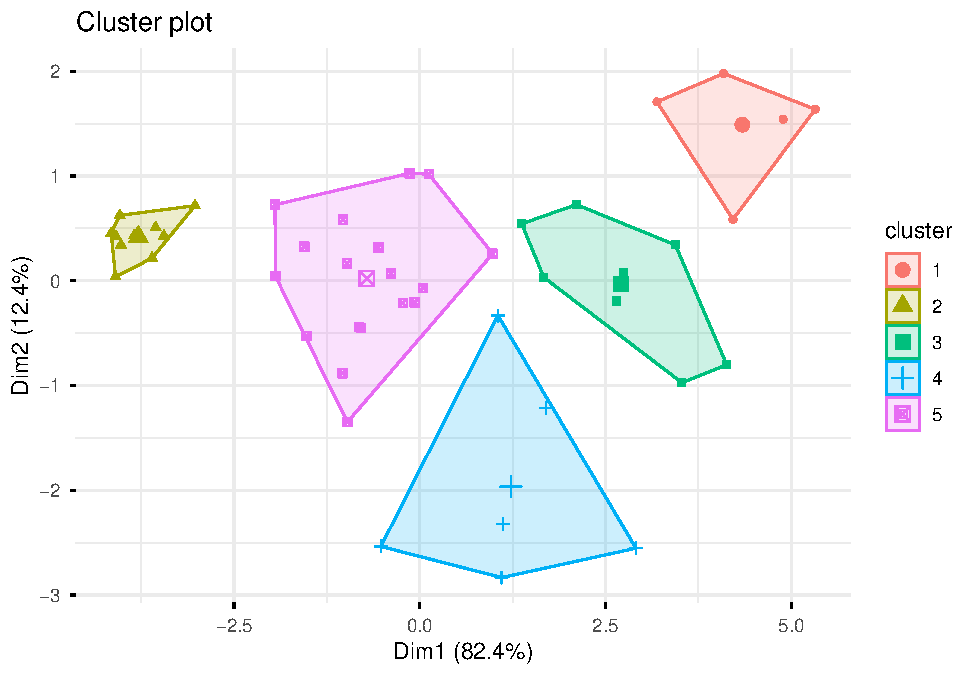
\includegraphics[keepaspectratio]{byHUC12_visual_ChatGPTv2_files/figure-latex/sens_summary-1.pdf}}

\begin{Shaded}
\begin{Highlighting}[]
\CommentTok{\# ============================================================}
\CommentTok{\# TREATMENT{-}PERFORMANCE ANALYSIS}
\CommentTok{\# ============================================================}
\CommentTok{\#}
\CommentTok{\# These metrics answer a different question from the landscape}
\CommentTok{\# classification: how do outcomes and implementation intensity}
\CommentTok{\# compare per hectare actually treated?}
\CommentTok{\# ============================================================}

\CommentTok{\# ============================================================}
\CommentTok{\# 23. Summarize PRIMARY planning classes}
\CommentTok{\# ============================================================}

\NormalTok{cluster\_summary }\OtherTok{\textless{}{-}}\NormalTok{ huc12\_planning }\SpecialCharTok{\%\textgreater{}\%}
  \FunctionTok{filter}\NormalTok{(}\SpecialCharTok{!}\FunctionTok{is.na}\NormalTok{(cluster)) }\SpecialCharTok{\%\textgreater{}\%}
  \FunctionTok{group\_by}\NormalTok{(cluster) }\SpecialCharTok{\%\textgreater{}\%}
  \FunctionTok{summarise}\NormalTok{(}

    \AttributeTok{n =} \FunctionTok{n}\NormalTok{(),}

    \CommentTok{\# Landscape transformation}
    \AttributeTok{mean\_per\_treated =}
      \FunctionTok{mean}\NormalTok{(per\_treated, }\AttributeTok{na.rm =} \ConstantTok{TRUE}\NormalTok{),}

    \CommentTok{\# Practice configuration}
    \AttributeTok{mean\_per\_patch =}
      \FunctionTok{mean}\NormalTok{(per\_patch, }\AttributeTok{na.rm =} \ConstantTok{TRUE}\NormalTok{),}

    \AttributeTok{mean\_per\_lin =}
      \FunctionTok{mean}\NormalTok{(per\_lin, }\AttributeTok{na.rm =} \ConstantTok{TRUE}\NormalTok{),}

    \AttributeTok{mean\_per\_rye =}
      \FunctionTok{mean}\NormalTok{(per\_rye, }\AttributeTok{na.rm =} \ConstantTok{TRUE}\NormalTok{),}

    \CommentTok{\# Landscape{-}scale outcomes}
    \AttributeTok{mean\_no3\_ha =}
      \FunctionTok{mean}\NormalTok{(no3\_ha, }\AttributeTok{na.rm =} \ConstantTok{TRUE}\NormalTok{),}

    \AttributeTok{mean\_sed\_ha =}
      \FunctionTok{mean}\NormalTok{(sed\_ha, }\AttributeTok{na.rm =} \ConstantTok{TRUE}\NormalTok{),}

    \AttributeTok{mean\_ghg\_ha =}
      \FunctionTok{mean}\NormalTok{(ghg\_ha, }\AttributeTok{na.rm =} \ConstantTok{TRUE}\NormalTok{),}

    \AttributeTok{mean\_bio\_Mg\_ha =}
      \FunctionTok{mean}\NormalTok{(bio\_Mg\_ha, }\AttributeTok{na.rm =} \ConstantTok{TRUE}\NormalTok{),}

    \CommentTok{\# Direct implementation cost}
    \AttributeTok{mean\_dccp\_ha =}
      \FunctionTok{mean}\NormalTok{(dccp\_ha, }\AttributeTok{na.rm =} \ConstantTok{TRUE}\NormalTok{),}

    \CommentTok{\# Opportunity cost {-}{-} CHARACTERIZATION ONLY}
    \AttributeTok{mean\_oc\_ha =}
      \FunctionTok{mean}\NormalTok{(oc\_ha, }\AttributeTok{na.rm =} \ConstantTok{TRUE}\NormalTok{),}

    \CommentTok{\# Total cost {-}{-} CHARACTERIZATION ONLY}
    \AttributeTok{mean\_tccp\_ha =}
      \FunctionTok{mean}\NormalTok{(tccp\_ha, }\AttributeTok{na.rm =} \ConstantTok{TRUE}\NormalTok{),}

    \CommentTok{\# Treatment{-}level outcomes}
    \AttributeTok{mean\_no3red =}
      \FunctionTok{mean}\NormalTok{(no3\_red, }\AttributeTok{na.rm =} \ConstantTok{TRUE}\NormalTok{),}

    \AttributeTok{mean\_sedred =}
      \FunctionTok{mean}\NormalTok{(sed\_red, }\AttributeTok{na.rm =} \ConstantTok{TRUE}\NormalTok{),}

    \AttributeTok{.groups =} \StringTok{"drop"}
\NormalTok{  )}

\FunctionTok{print}\NormalTok{(cluster\_summary)}
\end{Highlighting}
\end{Shaded}

\begin{verbatim}
## # A tibble: 5 x 15
##   cluster     n mean_per_treated mean_per_patch mean_per_lin mean_per_rye mean_no3_ha mean_sed_ha mean_ghg_ha mean_bio_Mg_ha mean_dccp_ha mean_oc_ha mean_tccp_ha mean_no3red mean_sedred
##   <fct>   <int>            <dbl>          <dbl>        <dbl>        <dbl>       <dbl>       <dbl>       <dbl>          <dbl>        <dbl>      <dbl>        <dbl>       <dbl>       <dbl>
## 1 1           5           0.477          0.0845      0.0544        0.333        16.5        3076.      0.747           2.45         318.       303.         413.        0.714      72075.
## 2 2          10           0.0522         0.0152      0.00418       0.0323        1.28        229.      0.0910          0.281         34.7       28.6         45.8       0.200      14157.
## 3 3           8           0.414          0.0873      0.0238        0.294        14.3        1870.      0.635           2.10         352.       292.         443.        0.607      61030.
## 4 4           6           0.307          0.149       0.0102        0.138        12.0         909.      0.642           1.83         285.       206.         396.        0.501      43811.
## 5 5          18           0.221          0.0601      0.0156        0.141         7.25        874.      0.373           1.17         174.       139.         223.        0.384      32268.
\end{verbatim}

\begin{Shaded}
\begin{Highlighting}[]
\FunctionTok{write.csv}\NormalTok{(}
\NormalTok{  cluster\_summary,}
  \StringTok{"../data/tidy/cluster\_summary.csv"}\NormalTok{,}
  \AttributeTok{row.names =} \ConstantTok{FALSE}
\NormalTok{)}

\CommentTok{\# {-}{-}{-}{-}{-}{-}{-}{-}{-}{-}{-}{-}{-}{-}{-}{-}{-}{-}{-}{-}{-}{-}{-}{-}{-}{-}{-}{-}{-}{-}{-}{-}{-}{-}{-}{-}{-}{-}{-}{-}{-}{-}{-}{-}{-}{-}{-}{-}{-}{-}{-}{-}{-}{-}{-}{-}{-}{-}{-}{-}}
\CommentTok{\# 10. Treatment{-}performance distributions}
\CommentTok{\# {-}{-}{-}{-}{-}{-}{-}{-}{-}{-}{-}{-}{-}{-}{-}{-}{-}{-}{-}{-}{-}{-}{-}{-}{-}{-}{-}{-}{-}{-}{-}{-}{-}{-}{-}{-}{-}{-}{-}{-}{-}{-}{-}{-}{-}{-}{-}{-}{-}{-}{-}{-}{-}{-}{-}{-}{-}{-}{-}{-}}
\NormalTok{facet2\_labels }\OtherTok{\textless{}{-}} \FunctionTok{c}\NormalTok{(}
  \AttributeTok{bio\_per\_treated\_ha   =} \StringTok{"atop(Biomass\textasciitilde{}Yield,(Mg\textasciitilde{}ha\^{}\{{-}1\}))"}\NormalTok{,}
  \AttributeTok{no3\_per\_treated\_ha      =} \StringTok{"atop(NO[3]\textasciitilde{}Load\textasciitilde{}Red.,(Mg\textasciitilde{}ha\^{}\{{-}1\}))"}\NormalTok{,}
  \AttributeTok{dccp\_per\_treated\_ha     =} \StringTok{"atop(Direct\textasciitilde{}Cost,(USD\textasciitilde{}ha\^{}\{{-}1\}))"}\NormalTok{,}
  \AttributeTok{oc\_per\_treated\_ha =} \StringTok{"atop(Opportunity\textasciitilde{}Cost,(USD\textasciitilde{}ha\^{}\{{-}1\}))"}\NormalTok{,}
  \AttributeTok{tccp\_per\_treated\_ha =} \StringTok{"atop(Total\textasciitilde{}Cost,(USD\textasciitilde{}ha\^{}\{{-}1\}))"}\NormalTok{,}
  \AttributeTok{sed\_per\_treated\_ha      =} \StringTok{"atop(Sed.\textasciitilde{}Load\textasciitilde{}Red.,(Mg\textasciitilde{}ha\^{}\{{-}1\}))"}\NormalTok{,}
  \AttributeTok{ghg\_per\_treated\_ha      =} \StringTok{"atop(GHG\textasciitilde{}Red.,(Mg\textasciitilde{}CO[2]*e\textasciitilde{}ha\^{}\{{-}1\}))"}\NormalTok{,}
  \AttributeTok{per\_treated =} \StringTok{"Treated\textasciitilde{}(\textquotesingle{}\%\textquotesingle{})"}\NormalTok{,}
  \AttributeTok{prairie\_share\_treated   =} \StringTok{"Prairie\textasciitilde{}(\textquotesingle{}\%\textquotesingle{})"}\NormalTok{,}
  \AttributeTok{rye\_share\_treated     =} \StringTok{"Cereal\textasciitilde{}Rye\textasciitilde{}(\textquotesingle{}\%\textquotesingle{})"}
\NormalTok{)}
\NormalTok{huc12\_planning }\SpecialCharTok{\%\textgreater{}\%}
  \FunctionTok{pivot\_longer}\NormalTok{(}
    \AttributeTok{cols =} \FunctionTok{c}\NormalTok{(}
\NormalTok{      no3\_per\_treated\_ha,}
\NormalTok{      sed\_per\_treated\_ha,}
\NormalTok{      ghg\_per\_treated\_ha,}
\NormalTok{      bio\_per\_treated\_ha,}
\NormalTok{      dccp\_per\_treated\_ha,}
\NormalTok{      rye\_share\_treated,}
\NormalTok{      prairie\_share\_treated,}
\NormalTok{      oc\_per\_treated\_ha,}
      
      \CommentTok{\#unprofit\_ha}
      \CommentTok{\#stabLow\_ha,}
\NormalTok{    ),}
    \AttributeTok{names\_to =} \StringTok{"Metric"}\NormalTok{,}
    \AttributeTok{values\_to =} \StringTok{"Value"}
\NormalTok{  ) }\SpecialCharTok{\%\textgreater{}\%}
  \FunctionTok{ggplot}\NormalTok{(}
    \FunctionTok{aes}\NormalTok{(}
      \AttributeTok{x =}\NormalTok{ Planning\_Class,}
      \AttributeTok{y =}\NormalTok{ Value,}
      \AttributeTok{fill =}\NormalTok{ Planning\_Class}
\NormalTok{    )}
\NormalTok{  ) }\SpecialCharTok{+}
  \FunctionTok{geom\_boxplot}\NormalTok{() }\SpecialCharTok{+}
  \FunctionTok{facet\_wrap}\NormalTok{(}\SpecialCharTok{\textasciitilde{}} \FunctionTok{factor}\NormalTok{(Metric, }\FunctionTok{c}\NormalTok{(}\StringTok{"no3\_per\_treated\_ha"}\NormalTok{,}\StringTok{"sed\_per\_treated\_ha"}\NormalTok{,}\StringTok{"ghg\_per\_treated\_ha"}\NormalTok{,}\StringTok{"bio\_per\_treated\_ha"}\NormalTok{,}\StringTok{"per\_treated"}\NormalTok{,}\StringTok{"rye\_share\_treated"}\NormalTok{,}\StringTok{"prairie\_share\_treated"}\NormalTok{,}\StringTok{"dccp\_per\_treated\_ha"}\NormalTok{,}\StringTok{"oc\_per\_treated\_ha"}\NormalTok{,}\StringTok{"tccp\_per\_treated\_ha"}\NormalTok{)), }\AttributeTok{scales =} \StringTok{"free\_y"}\NormalTok{,}\AttributeTok{ncol =} \DecValTok{2}\NormalTok{,,}
             \AttributeTok{strip.position =} \StringTok{"left"}\NormalTok{,}
             \AttributeTok{labeller =} \FunctionTok{as\_labeller}\NormalTok{(facet2\_labels, label\_parsed)) }\SpecialCharTok{+}
  \FunctionTok{ylab}\NormalTok{(}\ConstantTok{NULL}\NormalTok{) }\SpecialCharTok{+}
  \FunctionTok{theme\_minimal}\NormalTok{() }\SpecialCharTok{+}
  \FunctionTok{theme}\NormalTok{(}\AttributeTok{text =} \FunctionTok{element\_text}\NormalTok{(}\AttributeTok{family =} \StringTok{"serif"}\NormalTok{, }\AttributeTok{size =} \DecValTok{9}\NormalTok{),}
    \AttributeTok{axis.text.x =} \FunctionTok{element\_blank}\NormalTok{(),}
    \AttributeTok{strip.background =} \FunctionTok{element\_blank}\NormalTok{(),}
    \AttributeTok{strip.placement =} \StringTok{"outside"}
\NormalTok{  ) }\SpecialCharTok{+}
  \FunctionTok{scale\_fill\_manual}\NormalTok{(}\AttributeTok{values =} \FunctionTok{c}\NormalTok{(}\StringTok{\textquotesingle{}\#377EB8\textquotesingle{}}\NormalTok{,}\StringTok{\textquotesingle{}\#4DAF4A\textquotesingle{}}\NormalTok{,}\StringTok{\textquotesingle{}\#984EA3\textquotesingle{}}\NormalTok{,}\StringTok{\textquotesingle{}\#FF7F00\textquotesingle{}}\NormalTok{,}\StringTok{\textquotesingle{}\#FFFF33\textquotesingle{}}\NormalTok{), }
                    \CommentTok{\#labels = c("Nutrient{-}Biomass Integration", "Limited Environmental Intervention","Moderate Multifunctional Outcomes","Water{-}Quality{-}Biomass Integration","Prairie{-}Habitat{-}Nutrient Integration")}
\NormalTok{                    )}
\end{Highlighting}
\end{Shaded}

\pandocbounded{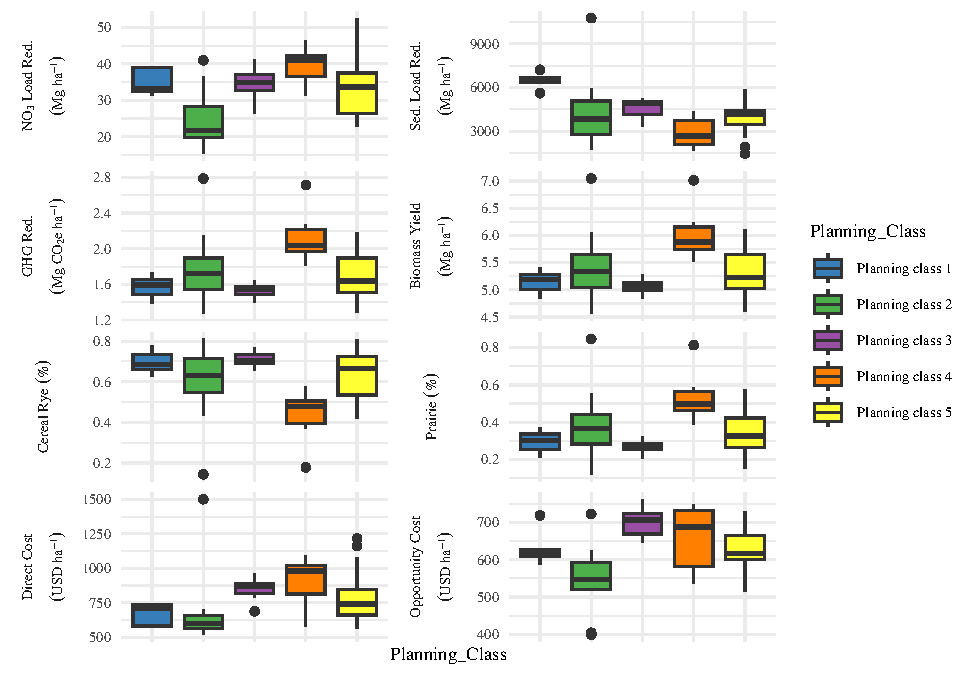
\includegraphics[keepaspectratio]{byHUC12_visual_ChatGPTv2_files/figure-latex/treatment_performance-1.pdf}}

\end{document}
